\documentclass{beamer}
\usepackage{tikz}
\usepackage[style=authoryear,backend=bibtex]{biblatex}
\usepackage{empheq}

\usetikzlibrary{arrows}
\usetikzlibrary{arrows.meta}
\usetikzlibrary{calc}
\usetikzlibrary{decorations.pathreplacing}
\usetikzlibrary{patterns}
\usetikzlibrary{positioning}
\usetikzlibrary{shapes}
\tikzstyle{every picture}+=[remember picture]
\tikzset{onslide/.code args={<#1>#2}{%
  \only<#1>{\pgfkeysalso{#2}}
}}

\usetheme{Singapore}
\usecolortheme{lily}
\beamertemplatenavigationsymbolsempty

\newcommand\independent{\protect\mathpalette{\protect\independenT}{\perp}}
\def\independenT#1#2{\mathrel{\rlap{$#1#2$}\mkern2mu{#1#2}}}

\DeclareMathOperator{\ifff}{:-}
\DeclareMathOperator{\prob}{::}
\DeclareMathOperator{\negg}{\backslash+}

\definecolor{predicate}{HTML}{1b9e77}
\definecolor{probability}{HTML}{e7298a}
\definecolor{variable}{HTML}{d95f02}
\definecolor{constant}{HTML}{7570b3}
\definecolor{color5}{HTML}{66a61e}
\definecolor{color6}{HTML}{e6ab02}

\addbibresource{talk.bib}

\author{\textbf{Paulius Dilkas}\inst{1} \and Vaishak Belle\inst{1,2}}
\title{Generating Random Logic Programs Using Constraint Programming}
\date{CP 2020}
\institute{\inst{1} University of Edinburgh, Edinburgh, UK \and \inst{2} Alan
  Turing Institute, London, UK}

\begin{document}

\begin{frame}[noframenumbering,plain]
  \tikz[remember picture,overlay]{
    \node at ([yshift=25pt,xshift=30pt]current page.south)
    {
\includegraphics[height=40pt]{inf.png}};
    \node at ([yshift=25pt,xshift=75pt]current page.south)
    {
\includegraphics[height=40pt]{ecr.jpg}};
    \node at ([yshift=20pt,xshift=140pt]current page.south)
    {
\includegraphics[height=20pt]{epsrc.png}};
  }
  \titlepage
\end{frame}

\section{Introduction}

\begin{frame}{Probabilistic Logic Programs (\textsc{ProbLog})}
  \begin{block}{``Smokers'' (\cite{DBLP:conf/ilp/DomingosKLPRS08,DBLP:journals/tplp/FierensBRSGTJR15})}
    \vspace*{-\baselineskip}\setlength\belowdisplayshortskip{0pt}
    \begin{align*}
      \textcolor{probability}{0.2} \prob &\textcolor{predicate}{\mathtt{stress}}(\textcolor{variable}{\mathsf{P}}) \ifff \textcolor{predicate}{\mathtt{person}}(\textcolor{variable}{\mathsf{P}}). \\
      \textcolor{probability}{0.3} \prob &\textcolor{predicate}{\mathtt{influences}}(\textcolor{variable}{\mathsf{P}_1}, \textcolor{variable}{\mathsf{P}_2}) \ifff \textcolor{predicate}{\mathtt{friend}}(\textcolor{variable}{\mathsf{P}_1}, \textcolor{variable}{\mathsf{P}_2}). \\
      \textcolor{probability}{0.1} \prob &\textcolor{predicate}{\mathtt{cancer\_spont}}(\textcolor{variable}{\mathsf{P}}) \ifff \textcolor{predicate}{\mathtt{person}}(\textcolor{variable}{\mathsf{P}}). \\
      \textcolor{probability}{0.3} \prob &\textcolor{predicate}{\mathtt{cancer\_smoke}}(\textcolor{variable}{\mathsf{P}}) \ifff \textcolor{predicate}{\mathtt{person}}(\textcolor{variable}{\mathsf{P}}). \\
                                         &\textcolor{predicate}{\mathtt{smokes}}(\textcolor{variable}{\mathsf{X}}) \ifff \textcolor{predicate}{\mathtt{stress}}(\textcolor{variable}{\mathsf{X}}). \\
                                         &\textcolor{predicate}{\mathtt{smokes}}(\textcolor{variable}{\mathsf{X}}) \ifff \textcolor{predicate}{\mathtt{smokes}}(\textcolor{variable}{\mathsf{Y}}), \textcolor{predicate}{\mathtt{influences}}(\textcolor{variable}{\mathsf{Y}}, \textcolor{variable}{\mathsf{X}}). \\
                                         &\textcolor{predicate}{\mathtt{cancer}}(\textcolor{variable}{\mathsf{P}}) \ifff \textcolor{predicate}{\mathtt{cancer\_spont}}(\textcolor{variable}{\mathsf{P}}). \\
                                         &\textcolor{predicate}{\mathtt{cancer}}(\textcolor{variable}{\mathsf{P}}) \ifff \textcolor{predicate}{\mathtt{smokes}}(\textcolor{variable}{\mathsf{P}}), \textcolor{predicate}{\mathtt{cancer\_smoke}}(\textcolor{variable}{\mathsf{P}}). \\
                                         &\textcolor{predicate}{\mathtt{person}}(\textcolor{constant}{\mathit{michelle}}). \\
                                         &\textcolor{predicate}{\mathtt{person}}(\textcolor{constant}{\mathit{timothy}}). \\
                                         &\textcolor{predicate}{\mathtt{friend}}(\textcolor{constant}{\mathit{timothy}}, \textcolor{constant}{\mathit{michelle}}).
    \end{align*}
  \end{block}
\end{frame}

\begin{frame}{Applications}
  \begin{columns}[b]
    \begin{column}{0.5\textwidth}
      \centering
      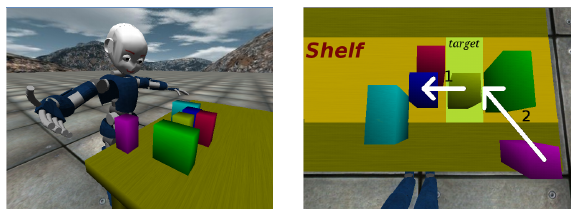
\includegraphics[width=\textwidth]{application1.png}
      {\small \cite{DBLP:conf/icra/MoldovanMOSR12}}
    \end{column}
    \begin{column}{0.5\textwidth}
      \centering
      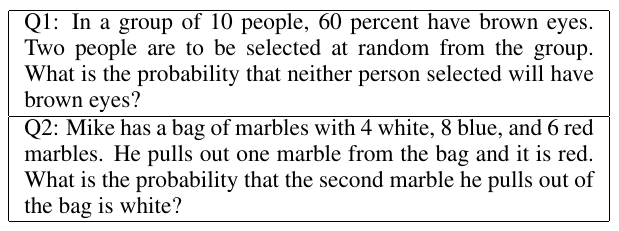
\includegraphics[width=\textwidth]{application3.png}
      {\small \cite{DBLP:conf/ijcai/DriesKDBR17}}
    \end{column}
  \end{columns}
  \vfill
  \begin{columns}[b]
    \begin{column}{0.5\textwidth}
      \centering
      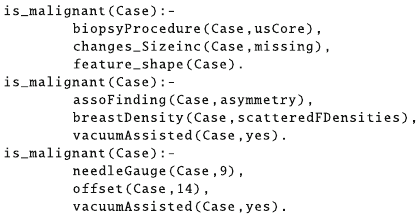
\includegraphics[width=\textwidth]{application2.png}
      {\small \cite{DBLP:conf/ilp/Corte-RealD017}}
    \end{column}
    \begin{column}{0.5\textwidth}
      \centering
      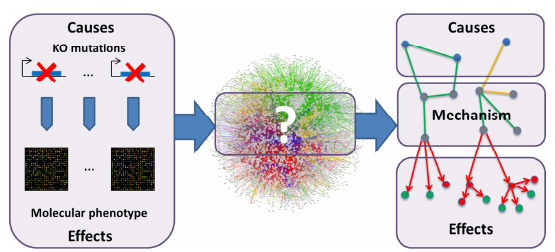
\includegraphics[width=\textwidth]{application4.png}
      {\small \cite{de2013phenetic}}
    \end{column}
  \end{columns}
\end{frame}

\begin{frame}{How Many Programs Are Used to Test Algorithms?}
  \begin{columns}
    \begin{column}{0.5\textwidth}
      \pause
      \fbox{
        \begin{tikzpicture}
          \node[inner sep = 0pt] (a) {
\includegraphics[width=\textwidth]{inference3.png}};
          \node[anchor=center] at (a.center) {\Huge\alert{4}};
        \end{tikzpicture}
      }
      \pause
      \fbox{
        \begin{tikzpicture}
          \node[inner sep = 0pt] (a) {
\includegraphics[width=\textwidth]{inference8.png}};
          \node[anchor=center] at (a.center) {\Huge\alert{3}};
        \end{tikzpicture}
      }
      \pause
      \fbox{
        \begin{tikzpicture}
          \node[inner sep = 0pt] (a) {
\includegraphics[width=\textwidth]{inference7.png}};
          \node[anchor=center] at (a.center) {\Huge\alert{1}};
        \end{tikzpicture}
      }
    \end{column}
    \begin{column}{0.5\textwidth}
      \pause
      \fbox{
        \begin{tikzpicture}
          \node[inner sep = 0pt] (a) {
\includegraphics[width=\textwidth]{inference6.png}};
          \node[anchor=center] at (a.center) {\Huge\alert{1}};
        \end{tikzpicture}
      }
      \pause
      \fbox{
        \begin{tikzpicture}
          \node[inner sep = 0pt] (a) {
\includegraphics[width=\textwidth]{inference2.png}};
          \node[anchor=center] at (a.center) {\Huge\alert{1}};
        \end{tikzpicture}
      }
      \pause
      \fbox{
        \begin{tikzpicture}
          \node[inner sep = 0pt] (a) {
\includegraphics[width=\textwidth]{inference1.png}};
          \node[anchor=center] at (a.center) {\Huge\alert{2}};
        \end{tikzpicture}
      }
    \end{column}
  \end{columns}
\end{frame}

\begin{frame}
  \frametitle{Outline}
  \tableofcontents
\end{frame}

\section{The Constraint Model}

\begin{frame}{What Characterizes a (Probabilistic) Logic Program?}
  \begin{columns}
    \hspace*{-0.7cm}\begin{column}{0.75\textwidth}
      \begin{empheq}[left =\onslide<6->{\color{color5}\empheqlbrace}]{equation}
        \begin{align*}
      \textcolor<5->{probability}{0.2} \prob &\textcolor<2->{predicate}{\mathtt{stress}}(\textcolor<3->{variable}{\mathsf{P}}) \ifff \textcolor<2->{predicate}{\mathtt{person}}(\textcolor<3->{variable}{\mathsf{P}}). \\
      \textcolor<5->{probability}{0.3} \prob &\textcolor<2->{predicate}{\mathtt{influences}}(\textcolor<3->{variable}{\mathsf{P}_1}, \textcolor<3->{variable}{\mathsf{P}_2}) \ifff \textcolor<2->{predicate}{\mathtt{friend}}(\textcolor<3->{variable}{\mathsf{P}_1}, \textcolor<3->{variable}{\mathsf{P}_2}). \\
      \textcolor<5->{probability}{0.1} \prob &\textcolor<2->{predicate}{\mathtt{cancer\_spont}}(\textcolor<3->{variable}{\mathsf{P}}) \ifff \textcolor<2->{predicate}{\mathtt{person}}(\textcolor<3->{variable}{\mathsf{P}}). \\
      \textcolor<5->{probability}{0.3} \prob &\textcolor<2->{predicate}{\mathtt{cancer\_smoke}}(\textcolor<3->{variable}{\mathsf{P}}) \ifff \textcolor<2->{predicate}{\mathtt{person}}(\textcolor<3->{variable}{\mathsf{P}}). \\
                                         &\textcolor<2->{predicate}{\mathtt{smokes}}(\textcolor<3->{variable}{\mathsf{X}}) \ifff \textcolor<2->{predicate}{\mathtt{stress}}(\textcolor<3->{variable}{\mathsf{X}}). \\
                                         &\textcolor<2->{predicate}{\mathtt{smokes}}(\textcolor<3->{variable}{\mathsf{X}}) \ifff \textcolor<2->{predicate}{\mathtt{smokes}}(\textcolor<3->{variable}{\mathsf{Y}}), \textcolor<2->{predicate}{\mathtt{influences}}(\textcolor<3->{variable}{\mathsf{Y}}, \textcolor<3->{variable}{\mathsf{X}}). \\
                                         &\textcolor<2->{predicate}{\mathtt{cancer}}(\textcolor<3->{variable}{\mathsf{P}}) \ifff \textcolor<2->{predicate}{\mathtt{cancer\_spont}}(\textcolor<3->{variable}{\mathsf{P}}). \\
                                         &\textcolor<2->{predicate}{\mathtt{cancer}}(\textcolor<3->{variable}{\mathsf{P}}) \ifff \tikz \coordinate (start);\textcolor<2->{predicate}{\mathtt{smokes}}(\textcolor<3->{variable}{\mathsf{P}}), \textcolor<2->{predicate}{\mathtt{cancer\_smoke}}(\textcolor<3->{variable}{\mathsf{P}})\tikz \coordinate (end);. \\
                                         &\textcolor<2->{predicate}{\mathtt{person}}(\textcolor<4->{constant}{\mathit{michelle}}). \\
                                         &\textcolor<2->{predicate}{\mathtt{person}}(\textcolor<4->{constant}{\mathit{timothy}}). \\
                                         &\textcolor<2->{predicate}{\mathtt{friend}}(\textcolor<4->{constant}{\mathit{timothy}}, \textcolor<4->{constant}{\mathit{michelle}}).
        \end{align*}
      \end{empheq}
    \end{column}
    \begin{column}{0.25\textwidth}
      \begin{itemize}
      \item[\textcolor{predicate}{\textbullet}]<2-> predicates, arities
      \item[\textcolor{variable}{\textbullet}]<3-> variables
      \item[\textcolor{constant}{\textbullet}]<4-> constants
      \item[\textcolor{probability}{\textbullet}]<5-> probabilities
      \item[\textcolor{color5}{\textbullet}]<6-> length
      \item[\textcolor{color6}{\textbullet}]<7-> complexity
      \end{itemize}
    \end{column}
  \end{columns}
  \onslide<7->{
    \begin{tikzpicture}[overlay]
      \draw [decorate,decoration={brace,amplitude=10pt,mirror},color=color6] (start) -- (end);
    \end{tikzpicture}
  }
\end{frame}

\begin{frame}{Formulas As Trees}
  \[
    \neg \textcolor{predicate}{\mathtt{p}}(\textcolor{variable}{\mathsf{X}})
    \lor (\textcolor{predicate}{\mathtt{q}}(\textcolor{variable}{\mathsf{X}})
    \land \textcolor{predicate}{\mathtt{r}}(\textcolor{variable}{\mathsf{X}}))
  \]
  \vfill
  \begin{columns}
    \begin{column}{0.5\textwidth}
      \pause
      \centering
      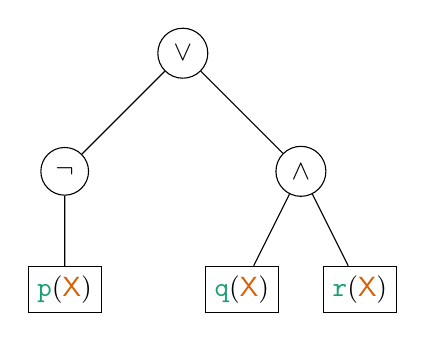
\begin{tikzpicture}[level 1/.style={sibling distance=30mm},level 2/.style={sibling distance=15mm}]
        \node[draw,circle] {$\lor$}
        child {node[draw,circle] {$\neg$}
          child {node[draw,rectangle] {$\textcolor{predicate}{\mathtt{p}}(\textcolor{variable}{\mathsf{X}})$}}
        }
        child {node[draw,circle] {$\land$}
          child {node[draw,rectangle] {$\textcolor{predicate}{\mathtt{q}}(\textcolor{variable}{\mathsf{X}})$}}
          child {node[draw,rectangle] {$\textcolor{predicate}{\mathtt{r}}(\textcolor{variable}{\mathsf{X}})$}}
        };
      \end{tikzpicture}
    \end{column}
    \begin{column}{0.5\textwidth}
      \pause
      \centering
      \begin{tabular}{|c|c|c|c|c|c|}
        \hline
        0\tikz \coordinate (disjunction2);&\tikz \coordinate (negation1);0\tikz \coordinate (negation2);&\tikz \coordinate (conjunction1);0\tikz \coordinate (conjunction2);&\tikz \coordinate (p);1 &\tikz \coordinate (q);2 &\tikz \coordinate (r);2 \\
        \hline
        $\lor$ & $\neg$ & $\land$ & $\textcolor{predicate}{\mathtt{p}}(\textcolor{variable}{\mathsf{X}})$ & $\textcolor{predicate}{\mathtt{q}}(\textcolor{variable}{\mathsf{X}})$ & $\textcolor{predicate}{\mathtt{r}}(\textcolor{variable}{\mathsf{X}})$ \\
        \hline
      \end{tabular}
      \begin{tikzpicture}[overlay]
        \draw[->,bend right=60,draw=red] ([yshift=0.75\baselineskip]negation1) to ([yshift=0.75\baselineskip]disjunction2);
        \draw[->,bend right=60,draw=red] ([yshift=0.75\baselineskip]conjunction1) to ([yshift=0.75\baselineskip]disjunction2);
        \draw[->,bend right=60,draw=red] ([yshift=0.75\baselineskip]p) to ([yshift=0.75\baselineskip]negation2);
        \draw[->,bend right=60,draw=red] ([yshift=0.75\baselineskip]q) to ([yshift=0.75\baselineskip]conjunction2);
        \draw[->,bend right=60,draw=red] ([yshift=0.75\baselineskip]r) to ([yshift=0.75\baselineskip]conjunction2);
      \end{tikzpicture}
    \end{column}
  \end{columns}
\end{frame}

\begin{frame}{Predicate Dependency Graph}
  \centering
  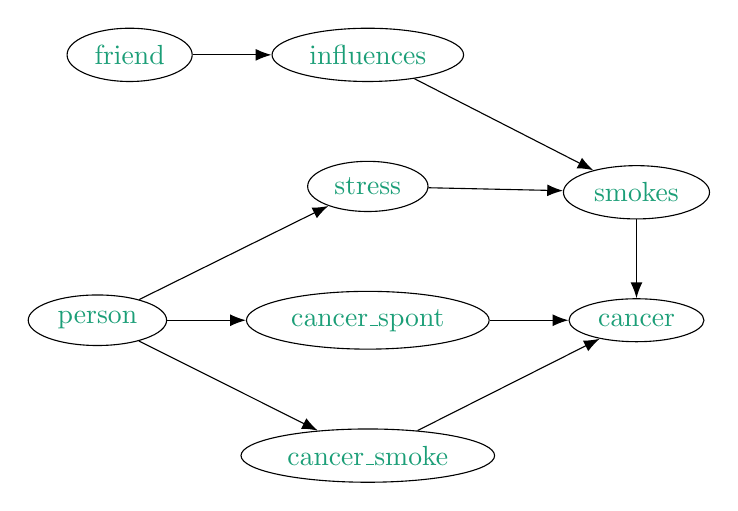
\begin{tikzpicture}
    \node[draw,ellipse] (friend) {\textcolor{predicate}{friend}};
    \node[draw,ellipse,right=of friend] (influences) {\textcolor{predicate}{influences}};
    \node[draw,ellipse,below=of influences] (stress) {\textcolor{predicate}{stress}};
    \node[draw,ellipse,below=of stress] (spont) {\textcolor{predicate}{cancer\_spont}};
    \node[draw,ellipse,below=of spont] (smoke) {\textcolor{predicate}{cancer\_smoke}};
    \node[draw,ellipse,left=of spont] (person) {\textcolor{predicate}{person}};
    \node[draw,ellipse,right=of spont] (cancer) {\textcolor{predicate}{cancer}};
    \node[draw,ellipse,above=of cancer] (smokes) {\textcolor{predicate}{smokes}};
    \draw[-{Latex[length=2mm]}] (friend) -- (influences);
    \draw[-{Latex[length=2mm]}] (influences) -- (smokes);
    \draw[-{Latex[length=2mm]}] (smokes) -- (cancer);
    \draw[-{Latex[length=2mm]}] (stress) -- (smokes);
    \draw[-{Latex[length=2mm]}] (spont) -- (cancer);
    \draw[-{Latex[length=2mm]}] (smoke) -- (cancer);
    \draw[-{Latex[length=2mm]}] (person) -- (stress);
    \draw[-{Latex[length=2mm]}] (person) -- (spont);
    \draw[-{Latex[length=2mm]}] (person) -- (smoke);
  \end{tikzpicture}
\end{frame}

\begin{frame}{Stratification and Negative Cycles}
  \[
    \textcolor{probability}{0.1} \prob
    \textcolor{predicate}{\mathtt{friend}}(\textcolor{variable}{\mathsf{X}},
    \textcolor{variable}{\mathsf{Y}}) \ifff
    \negg\textcolor{predicate}{\mathtt{smokes}}(\textcolor{variable}{\mathsf{Y}}).
  \]
  \vfill
%  \begin{columns}
%    \begin{column}{0.4\textwidth}
%      \setlength{\leftmargini}{0pt}
%      \begin{itemize}
%      \item<3-> \alert{Stratum 1}: predicates with no negation
%      \item<3-> \alert{Stratum 2}: new predicates s.t. negative literals refer to
%        predicates in \alert{Stratum~1}
%      \end{itemize}
%      \vspace{5em}
%    \end{column}
%    \begin{column}{0.6\textwidth}
%      \hspace{-6.92em}
  \centering
      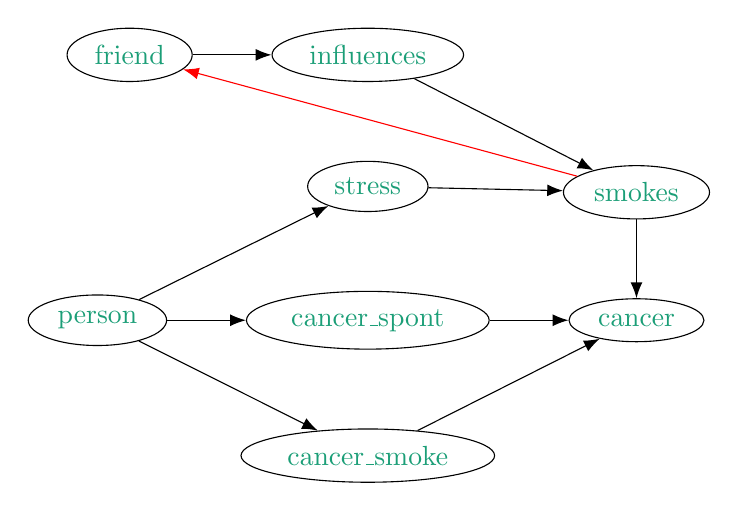
\begin{tikzpicture}
        \node[draw,ellipse] (friend) {\textcolor{predicate}{friend}};
        \node[draw,ellipse,right=of friend] (influences) {\textcolor{predicate}{influences}};
        \node[draw,ellipse,below=of influences] (stress) {\textcolor{predicate}{stress}};
        \node[draw,ellipse,below=of stress] (spont) {\textcolor{predicate}{cancer\_spont}};
        \node[draw,ellipse,below=of spont] (smoke) {\textcolor{predicate}{cancer\_smoke}};
        \node[draw,ellipse,left=of spont] (person) {\textcolor{predicate}{person}};
        \node[draw,ellipse,right=of spont] (cancer) {\textcolor{predicate}{cancer}};
        \node[draw,ellipse,above=of cancer] (smokes) {\textcolor{predicate}{smokes}};
        \draw[-{Latex[length=2mm]}] (friend) -- (influences);
        \draw[-{Latex[length=2mm]}] (influences) -- (smokes);
        \draw[-{Latex[length=2mm]}] (smokes) -- (cancer);
        \draw[-{Latex[length=2mm]}] (stress) -- (smokes);
        \draw[-{Latex[length=2mm]}] (spont) -- (cancer);
        \draw[-{Latex[length=2mm]}] (smoke) -- (cancer);
        \draw[-{Latex[length=2mm]}] (person) -- (stress);
        \draw[-{Latex[length=2mm]}] (person) -- (spont);
        \draw[-{Latex[length=2mm]}] (person) -- (smoke);
        \draw<2->[-{Latex[length=2mm]},draw=red] (smokes) -- (friend);
      \end{tikzpicture}
%    \end{column}
%  \end{columns}
\end{frame}

\begin{frame}{Predicate Independence: $\textcolor{predicate}{\mathrm{friend}}
    \independent \textcolor{predicate}{\mathrm{stress}}$}
  \centering
  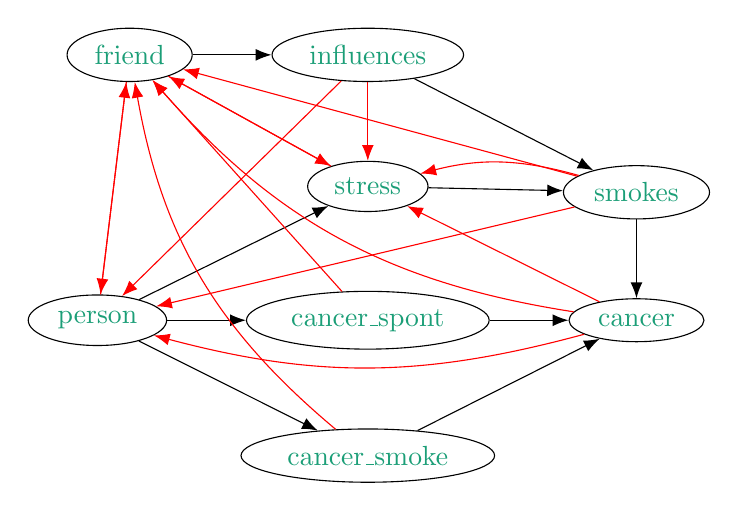
\begin{tikzpicture}
    \node[draw,ellipse,onslide=<2->{fill=constant!25}] (friend) {\textcolor{predicate}{friend}};
    \node[draw,ellipse,right=of friend,onslide=<5-6>{pattern=north east lines,pattern color=constant}] (influences) {\textcolor{predicate}{influences}};
    \node[draw,ellipse,onslide=<2->{fill=variable!25},below=of influences] (stress) {\textcolor{predicate}{stress}};
    \node[draw,ellipse,below=of stress,onslide=<3-4>{pattern=north west lines,pattern color=variable}] (spont) {\textcolor{predicate}{cancer\_spont}};
    \node[draw,ellipse,below=of spont,onslide=<3-4>{pattern=north west lines,pattern color=variable}] (smoke) {\textcolor{predicate}{cancer\_smoke}};
    \node[draw,ellipse,onslide=<2->{fill=variable!25},left=of spont] (person) {\textcolor{predicate}{person}};
    \node[draw,ellipse,right=of spont,onslide=<3-4>{pattern=north west lines,pattern color=variable},onslide=<5-6>{pattern=north east lines,pattern color=constant}] (cancer) {\textcolor{predicate}{cancer}};
    \node[draw,ellipse,above=of cancer,onslide=<3-4>{pattern=north west lines,pattern color=variable},onslide=<5-6>{pattern=north east lines,pattern color=constant}] (smokes) {\textcolor{predicate}{smokes}};
    \draw[-{Latex[length=2mm]}] (friend) -- (influences);
    \draw[-{Latex[length=2mm]}] (influences) -- (smokes);
    \draw[-{Latex[length=2mm]}] (smokes) -- (cancer);
    \draw[-{Latex[length=2mm]}] (stress) -- (smokes);
    \draw[-{Latex[length=2mm]}] (spont) -- (cancer);
    \draw[-{Latex[length=2mm]}] (smoke) -- (cancer);
    \draw[-{Latex[length=2mm]}] (person) -- (stress);
    \draw[-{Latex[length=2mm]}] (person) -- (spont);
    \draw[-{Latex[length=2mm]}] (person) -- (smoke);

    \draw<4>[-{Latex[length=2mm]}] (person) edge[draw=red] (friend);
    \draw<4>[-{Latex[length=2mm]}] (stress) edge[draw=red] (friend);
    \draw<4>[-{Latex[length=2mm]}] (smokes) edge[draw=red] (friend);
    \draw<4>[-{Latex[length=2mm]}] (spont) edge[draw=red] (friend);
    \draw<4>[-{Latex[length=2mm]}] (cancer) edge[draw=red,bend left=20] (friend);
    \draw<4>[-{Latex[length=2mm]}] (smoke) edge[draw=red,bend left=20] (friend);

    \draw<6>[-{Latex[length=2mm]}] (friend) edge[draw=red] (person);
    \draw<6>[-{Latex[length=2mm]}] (influences) edge[draw=red] (person);
    \draw<6>[-{Latex[length=2mm]}] (smokes) edge[draw=red] (person);
    \draw<6>[-{Latex[length=2mm]}] (cancer) edge[draw=red,bend left=15] (person);

    \draw<6>[-{Latex[length=2mm]}] (friend) edge[draw=red] (stress);
    \draw<6>[-{Latex[length=2mm]}] (influences) edge[draw=red] (stress);
    \draw<6>[-{Latex[length=2mm]}] (smokes) edge[draw=red,bend right=15] (stress);
    \draw<6>[-{Latex[length=2mm]}] (cancer) edge[draw=red] (stress);
  \end{tikzpicture}
\end{frame}

\begin{frame}{Scalability}
  \centering
  % Created by tikzDevice version 0.12.3 on 2020-05-11 12:44:46
% !TEX encoding = UTF-8 Unicode
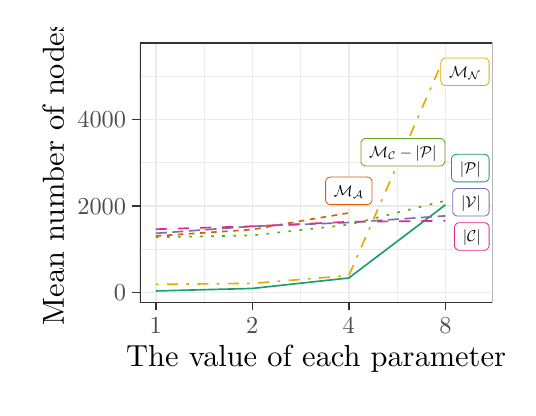
\begin{tikzpicture}[x=1pt,y=1pt]
\definecolor{fillColor}{RGB}{255,255,255}
\path[use as bounding box,fill=fillColor,fill opacity=0.00] (0,0) rectangle (173.45,130.09);
\begin{scope}
\path[clip] (  0.00,  0.00) rectangle (173.45,130.09);
\definecolor{drawColor}{RGB}{255,255,255}
\definecolor{fillColor}{RGB}{255,255,255}

\path[draw=drawColor,line width= 0.6pt,line join=round,line cap=round,fill=fillColor] (  0.00,  0.00) rectangle (173.45,130.09);
\end{scope}
\begin{scope}
\path[clip] ( 40.51, 30.69) rectangle (167.95,124.59);
\definecolor{fillColor}{RGB}{255,255,255}

\path[fill=fillColor] ( 40.51, 30.69) rectangle (167.95,124.59);
\definecolor{drawColor}{gray}{0.92}

\path[draw=drawColor,line width= 0.3pt,line join=round] ( 40.51, 50.03) --
	(167.95, 50.03);

\path[draw=drawColor,line width= 0.3pt,line join=round] ( 40.51, 81.30) --
	(167.95, 81.30);

\path[draw=drawColor,line width= 0.3pt,line join=round] ( 40.51,112.57) --
	(167.95,112.57);

\path[draw=drawColor,line width= 0.3pt,line join=round] ( 63.74, 30.69) --
	( 63.74,124.59);

\path[draw=drawColor,line width= 0.3pt,line join=round] ( 98.62, 30.69) --
	( 98.62,124.59);

\path[draw=drawColor,line width= 0.3pt,line join=round] (133.49, 30.69) --
	(133.49,124.59);

\path[draw=drawColor,line width= 0.6pt,line join=round] ( 40.51, 34.40) --
	(167.95, 34.40);

\path[draw=drawColor,line width= 0.6pt,line join=round] ( 40.51, 65.67) --
	(167.95, 65.67);

\path[draw=drawColor,line width= 0.6pt,line join=round] ( 40.51, 96.94) --
	(167.95, 96.94);

\path[draw=drawColor,line width= 0.6pt,line join=round] ( 46.30, 30.69) --
	( 46.30,124.59);

\path[draw=drawColor,line width= 0.6pt,line join=round] ( 81.18, 30.69) --
	( 81.18,124.59);

\path[draw=drawColor,line width= 0.6pt,line join=round] (116.05, 30.69) --
	(116.05,124.59);

\path[draw=drawColor,line width= 0.6pt,line join=round] (150.93, 30.69) --
	(150.93,124.59);
\definecolor{drawColor}{RGB}{27,158,119}

\path[draw=drawColor,line width= 0.6pt,line join=round] ( 46.30, 34.95) --
	( 81.18, 35.86) --
	(116.05, 39.64) --
	(150.93, 66.05);
\definecolor{drawColor}{RGB}{217,95,2}

\path[draw=drawColor,line width= 0.6pt,dash pattern=on 2pt off 2pt ,line join=round] ( 46.30, 54.81) --
	( 81.18, 57.14) --
	(101.58, 60.74) --
	(116.05, 63.15);
\definecolor{drawColor}{RGB}{117,112,179}

\path[draw=drawColor,line width= 0.6pt,dash pattern=on 4pt off 2pt ,line join=round] ( 46.30, 55.77) --
	( 81.18, 58.31) --
	(116.05, 59.68) --
	(150.93, 62.08);
\definecolor{drawColor}{RGB}{231,41,138}

\path[draw=drawColor,line width= 0.6pt,dash pattern=on 4pt off 4pt ,line join=round] ( 46.30, 57.27) --
	( 81.18, 58.33) --
	(116.05, 59.95) --
	(150.93, 60.30);
\definecolor{drawColor}{RGB}{102,166,30}

\path[draw=drawColor,line width= 0.6pt,dash pattern=on 1pt off 3pt ,line join=round] ( 46.30, 54.34) --
	( 81.18, 55.03) --
	(116.05, 58.92) --
	(150.93, 67.56);
\definecolor{drawColor}{RGB}{230,171,2}

\path[draw=drawColor,line width= 0.6pt,dash pattern=on 1pt off 3pt on 4pt off 3pt ,line join=round] ( 46.30, 37.33) --
	( 81.18, 37.69) --
	(116.05, 40.51) --
	(150.93,120.32);
\end{scope}
\begin{scope}
\path[clip] ( 40.51, 30.69) rectangle (167.95,124.59);

\path[] (158.55, 74.38) -- (150.93, 66.05);
\definecolor{drawColor}{RGB}{27,158,119}
\definecolor{fillColor}{RGB}{255,255,255}

\path[draw=drawColor,line width= 0.3pt,line join=round,line cap=round,fill=fillColor] (154.94, 74.38) --
	(164.94, 74.38) --
	(164.86, 74.38) --
	(165.15, 74.39) --
	(165.44, 74.45) --
	(165.71, 74.55) --
	(165.96, 74.70) --
	(166.19, 74.88) --
	(166.38, 75.10) --
	(166.54, 75.34) --
	(166.65, 75.61) --
	(166.72, 75.89) --
	(166.74, 76.18) --
	(166.74, 76.18) --
	(166.74, 82.51) --
	(166.74, 82.51) --
	(166.72, 82.80) --
	(166.65, 83.08) --
	(166.54, 83.35) --
	(166.38, 83.60) --
	(166.19, 83.81) --
	(165.96, 84.00) --
	(165.71, 84.14) --
	(165.44, 84.25) --
	(165.15, 84.30) --
	(164.94, 84.32) --
	(154.94, 84.32) --
	(155.16, 84.30) --
	(154.87, 84.32) --
	(154.58, 84.28) --
	(154.30, 84.20) --
	(154.04, 84.08) --
	(153.80, 83.91) --
	(153.59, 83.71) --
	(153.41, 83.48) --
	(153.28, 83.22) --
	(153.19, 82.94) --
	(153.14, 82.66) --
	(153.13, 82.51) --
	(153.13, 76.18) --
	(153.14, 76.33) --
	(153.14, 76.04) --
	(153.19, 75.75) --
	(153.28, 75.47) --
	(153.41, 75.22) --
	(153.59, 74.98) --
	(153.80, 74.78) --
	(154.04, 74.62) --
	(154.30, 74.49) --
	(154.58, 74.41) --
	(154.87, 74.38) --
	cycle;
\end{scope}
\begin{scope}
\path[clip] ( 40.51, 30.69) rectangle (167.95,124.59);
\definecolor{drawColor}{RGB}{27,158,119}

\node[text=black,anchor=base,inner sep=0pt, outer sep=0pt, scale=  0.57] at (159.94, 77.39) {$|\mathcal{P}|$};
\end{scope}
\begin{scope}
\path[clip] ( 40.51, 30.69) rectangle (167.95,124.59);
\definecolor{drawColor}{RGB}{117,112,179}
\definecolor{fillColor}{RGB}{255,255,255}

\path[draw=drawColor,line width= 0.3pt,line join=round,line cap=round,fill=fillColor] (155.41, 62.03) --
	(164.94, 62.03) --
	(164.86, 62.03) --
	(165.15, 62.04) --
	(165.44, 62.10) --
	(165.71, 62.20) --
	(165.96, 62.35) --
	(166.19, 62.53) --
	(166.38, 62.75) --
	(166.53, 63.00) --
	(166.65, 63.26) --
	(166.72, 63.55) --
	(166.74, 63.84) --
	(166.74, 63.84) --
	(166.74, 70.16) --
	(166.74, 70.16) --
	(166.72, 70.45) --
	(166.65, 70.74) --
	(166.53, 71.00) --
	(166.38, 71.25) --
	(166.19, 71.47) --
	(165.96, 71.65) --
	(165.71, 71.80) --
	(165.44, 71.90) --
	(165.15, 71.96) --
	(164.94, 71.97) --
	(155.41, 71.97) --
	(155.63, 71.96) --
	(155.34, 71.97) --
	(155.05, 71.93) --
	(154.77, 71.85) --
	(154.51, 71.73) --
	(154.27, 71.56) --
	(154.06, 71.36) --
	(153.88, 71.13) --
	(153.75, 70.87) --
	(153.65, 70.60) --
	(153.61, 70.31) --
	(153.60, 70.16) --
	(153.60, 63.84) --
	(153.61, 63.98) --
	(153.61, 63.69) --
	(153.65, 63.40) --
	(153.75, 63.13) --
	(153.88, 62.87) --
	(154.06, 62.64) --
	(154.27, 62.44) --
	(154.51, 62.27) --
	(154.77, 62.15) --
	(155.05, 62.07) --
	(155.34, 62.03) --
	cycle;
\end{scope}
\begin{scope}
\path[clip] ( 40.51, 30.69) rectangle (167.95,124.59);
\definecolor{drawColor}{RGB}{117,112,179}

\node[text=black,anchor=base,inner sep=0pt, outer sep=0pt, scale=  0.57] at (160.17, 65.04) {$|\mathcal{V}|$};
\end{scope}
\begin{scope}
\path[clip] ( 40.51, 30.69) rectangle (167.95,124.59);
\definecolor{drawColor}{RGB}{231,41,138}
\definecolor{fillColor}{RGB}{255,255,255}

\path[draw=drawColor,line width= 0.3pt,line join=round,line cap=round,fill=fillColor] (156.04, 49.68) --
	(164.94, 49.68) --
	(164.86, 49.68) --
	(165.15, 49.69) --
	(165.44, 49.75) --
	(165.71, 49.85) --
	(165.96, 50.00) --
	(166.19, 50.18) --
	(166.38, 50.40) --
	(166.54, 50.65) --
	(166.65, 50.91) --
	(166.72, 51.20) --
	(166.74, 51.49) --
	(166.74, 51.49) --
	(166.74, 57.81) --
	(166.74, 57.81) --
	(166.72, 58.10) --
	(166.65, 58.39) --
	(166.54, 58.65) --
	(166.38, 58.90) --
	(166.19, 59.12) --
	(165.96, 59.30) --
	(165.71, 59.45) --
	(165.44, 59.55) --
	(165.15, 59.61) --
	(164.94, 59.62) --
	(156.04, 59.62) --
	(156.26, 59.61) --
	(155.96, 59.62) --
	(155.68, 59.58) --
	(155.40, 59.50) --
	(155.13, 59.38) --
	(154.89, 59.21) --
	(154.69, 59.01) --
	(154.51, 58.78) --
	(154.38, 58.52) --
	(154.28, 58.25) --
	(154.24, 57.96) --
	(154.23, 57.81) --
	(154.23, 51.49) --
	(154.24, 51.63) --
	(154.24, 51.34) --
	(154.28, 51.05) --
	(154.38, 50.78) --
	(154.51, 50.52) --
	(154.69, 50.29) --
	(154.89, 50.09) --
	(155.13, 49.92) --
	(155.40, 49.80) --
	(155.68, 49.72) --
	(155.96, 49.68) --
	cycle;
\end{scope}
\begin{scope}
\path[clip] ( 40.51, 30.69) rectangle (167.95,124.59);
\definecolor{drawColor}{RGB}{231,41,138}

\node[text=black,anchor=base,inner sep=0pt, outer sep=0pt, scale=  0.57] at (160.49, 52.69) {$|\mathcal{C}|$};
\end{scope}
\begin{scope}
\path[clip] ( 40.51, 30.69) rectangle (167.95,124.59);

\path[] (139.49, 80.12) -- (150.93, 67.56);
\definecolor{drawColor}{RGB}{102,166,30}
\definecolor{fillColor}{RGB}{255,255,255}

\path[draw=drawColor,line width= 0.3pt,line join=round,line cap=round,fill=fillColor] (122.22, 80.12) --
	(148.97, 80.12) --
	(148.89, 80.12) --
	(149.18, 80.13) --
	(149.47, 80.19) --
	(149.74, 80.29) --
	(149.99, 80.44) --
	(150.22, 80.62) --
	(150.41, 80.84) --
	(150.57, 81.08) --
	(150.68, 81.35) --
	(150.75, 81.63) --
	(150.77, 81.92) --
	(150.77, 81.92) --
	(150.77, 88.25) --
	(150.77, 88.25) --
	(150.75, 88.54) --
	(150.68, 88.82) --
	(150.57, 89.09) --
	(150.41, 89.34) --
	(150.22, 89.55) --
	(149.99, 89.74) --
	(149.74, 89.88) --
	(149.47, 89.99) --
	(149.18, 90.05) --
	(148.97, 90.06) --
	(122.22, 90.06) --
	(122.44, 90.05) --
	(122.15, 90.06) --
	(121.86, 90.02) --
	(121.58, 89.94) --
	(121.32, 89.82) --
	(121.08, 89.65) --
	(120.87, 89.45) --
	(120.70, 89.22) --
	(120.56, 88.96) --
	(120.47, 88.68) --
	(120.42, 88.40) --
	(120.42, 88.25) --
	(120.42, 81.92) --
	(120.42, 82.07) --
	(120.42, 81.78) --
	(120.47, 81.49) --
	(120.56, 81.21) --
	(120.70, 80.96) --
	(120.87, 80.72) --
	(121.08, 80.52) --
	(121.32, 80.36) --
	(121.58, 80.23) --
	(121.86, 80.15) --
	(122.15, 80.12) --
	cycle;
\end{scope}
\begin{scope}
\path[clip] ( 40.51, 30.69) rectangle (167.95,124.59);
\definecolor{drawColor}{RGB}{102,166,30}

\node[text=black,anchor=base,inner sep=0pt, outer sep=0pt, scale=  0.57] at (135.59, 83.13) {$\mathcal{M}_{\mathcal{C}}-|\mathcal{P}|$};
\end{scope}
\begin{scope}
\path[clip] ( 40.51, 30.69) rectangle (167.95,124.59);
\definecolor{drawColor}{RGB}{230,171,2}
\definecolor{fillColor}{RGB}{255,255,255}

\path[draw=drawColor,line width= 0.3pt,line join=round,line cap=round,fill=fillColor] (151.08,109.18) --
	(164.94,109.18) --
	(164.86,109.18) --
	(165.15,109.19) --
	(165.44,109.25) --
	(165.71,109.36) --
	(165.96,109.50) --
	(166.19,109.68) --
	(166.38,109.90) --
	(166.54,110.15) --
	(166.65,110.42) --
	(166.72,110.70) --
	(166.74,110.99) --
	(166.74,110.99) --
	(166.74,117.32) --
	(166.74,117.32) --
	(166.72,117.61) --
	(166.65,117.89) --
	(166.54,118.16) --
	(166.38,118.40) --
	(166.19,118.62) --
	(165.96,118.80) --
	(165.71,118.95) --
	(165.44,119.05) --
	(165.15,119.11) --
	(164.94,119.12) --
	(151.08,119.12) --
	(151.30,119.11) --
	(151.01,119.12) --
	(150.72,119.09) --
	(150.44,119.01) --
	(150.18,118.88) --
	(149.94,118.72) --
	(149.73,118.51) --
	(149.56,118.28) --
	(149.42,118.02) --
	(149.33,117.75) --
	(149.28,117.46) --
	(149.28,117.32) --
	(149.28,110.99) --
	(149.28,111.13) --
	(149.28,110.84) --
	(149.33,110.56) --
	(149.42,110.28) --
	(149.56,110.02) --
	(149.73,109.79) --
	(149.94,109.59) --
	(150.18,109.42) --
	(150.44,109.30) --
	(150.72,109.22) --
	(151.01,109.18) --
	cycle;
\end{scope}
\begin{scope}
\path[clip] ( 40.51, 30.69) rectangle (167.95,124.59);
\definecolor{drawColor}{RGB}{230,171,2}

\node[text=black,anchor=base,inner sep=0pt, outer sep=0pt, scale=  0.57] at (158.01,112.19) {$\mathcal{M}_{\mathcal{N}}$};
\end{scope}
\begin{scope}
\path[clip] ( 40.51, 30.69) rectangle (167.95,124.59);
\definecolor{drawColor}{RGB}{217,95,2}
\definecolor{fillColor}{RGB}{255,255,255}

\path[draw=drawColor,line width= 0.3pt,line join=round,line cap=round,fill=fillColor] (109.46, 66.16) --
	(122.64, 66.16) --
	(122.57, 66.16) --
	(122.86, 66.17) --
	(123.15, 66.23) --
	(123.42, 66.33) --
	(123.67, 66.48) --
	(123.90, 66.66) --
	(124.09, 66.88) --
	(124.24, 67.12) --
	(124.36, 67.39) --
	(124.43, 67.67) --
	(124.45, 67.96) --
	(124.45, 67.96) --
	(124.45, 74.29) --
	(124.45, 74.29) --
	(124.43, 74.58) --
	(124.36, 74.86) --
	(124.24, 75.13) --
	(124.09, 75.38) --
	(123.90, 75.60) --
	(123.67, 75.78) --
	(123.42, 75.92) --
	(123.15, 76.03) --
	(122.86, 76.09) --
	(122.64, 76.10) --
	(109.46, 76.10) --
	(109.68, 76.09) --
	(109.39, 76.10) --
	(109.10, 76.06) --
	(108.82, 75.98) --
	(108.56, 75.86) --
	(108.32, 75.69) --
	(108.11, 75.49) --
	(107.93, 75.26) --
	(107.80, 75.00) --
	(107.71, 74.72) --
	(107.66, 74.44) --
	(107.65, 74.29) --
	(107.65, 67.96) --
	(107.66, 68.11) --
	(107.66, 67.82) --
	(107.71, 67.53) --
	(107.80, 67.26) --
	(107.93, 67.00) --
	(108.11, 66.77) --
	(108.32, 66.56) --
	(108.56, 66.40) --
	(108.82, 66.27) --
	(109.10, 66.19) --
	(109.39, 66.16) --
	cycle;
\end{scope}
\begin{scope}
\path[clip] ( 40.51, 30.69) rectangle (167.95,124.59);
\definecolor{drawColor}{RGB}{217,95,2}

\node[text=black,anchor=base,inner sep=0pt, outer sep=0pt, scale=  0.57] at (116.05, 69.17) {$\mathcal{M}_{\mathcal{A}}$};
\definecolor{drawColor}{gray}{0.20}

\path[draw=drawColor,line width= 0.6pt,line join=round,line cap=round] ( 40.51, 30.69) rectangle (167.95,124.59);
\end{scope}
\begin{scope}
\path[clip] (  0.00,  0.00) rectangle (173.45,130.09);
\definecolor{drawColor}{gray}{0.30}

\node[text=drawColor,anchor=base east,inner sep=0pt, outer sep=0pt, scale=  0.88] at ( 35.56, 31.37) {0};

\node[text=drawColor,anchor=base east,inner sep=0pt, outer sep=0pt, scale=  0.88] at ( 35.56, 62.64) {2000};

\node[text=drawColor,anchor=base east,inner sep=0pt, outer sep=0pt, scale=  0.88] at ( 35.56, 93.91) {4000};
\end{scope}
\begin{scope}
\path[clip] (  0.00,  0.00) rectangle (173.45,130.09);
\definecolor{drawColor}{gray}{0.20}

\path[draw=drawColor,line width= 0.6pt,line join=round] ( 37.76, 34.40) --
	( 40.51, 34.40);

\path[draw=drawColor,line width= 0.6pt,line join=round] ( 37.76, 65.67) --
	( 40.51, 65.67);

\path[draw=drawColor,line width= 0.6pt,line join=round] ( 37.76, 96.94) --
	( 40.51, 96.94);
\end{scope}
\begin{scope}
\path[clip] (  0.00,  0.00) rectangle (173.45,130.09);
\definecolor{drawColor}{gray}{0.20}

\path[draw=drawColor,line width= 0.6pt,line join=round] ( 46.30, 27.94) --
	( 46.30, 30.69);

\path[draw=drawColor,line width= 0.6pt,line join=round] ( 81.18, 27.94) --
	( 81.18, 30.69);

\path[draw=drawColor,line width= 0.6pt,line join=round] (116.05, 27.94) --
	(116.05, 30.69);

\path[draw=drawColor,line width= 0.6pt,line join=round] (150.93, 27.94) --
	(150.93, 30.69);
\end{scope}
\begin{scope}
\path[clip] (  0.00,  0.00) rectangle (173.45,130.09);
\definecolor{drawColor}{gray}{0.30}

\node[text=drawColor,anchor=base,inner sep=0pt, outer sep=0pt, scale=  0.88] at ( 46.30, 19.68) {1};

\node[text=drawColor,anchor=base,inner sep=0pt, outer sep=0pt, scale=  0.88] at ( 81.18, 19.68) {2};

\node[text=drawColor,anchor=base,inner sep=0pt, outer sep=0pt, scale=  0.88] at (116.05, 19.68) {4};

\node[text=drawColor,anchor=base,inner sep=0pt, outer sep=0pt, scale=  0.88] at (150.93, 19.68) {8};
\end{scope}
\begin{scope}
\path[clip] (  0.00,  0.00) rectangle (173.45,130.09);
\definecolor{drawColor}{RGB}{0,0,0}

\node[text=drawColor,anchor=base,inner sep=0pt, outer sep=0pt, scale=  1.10] at (104.23,  7.64) {The value of each parameter};
\end{scope}
\begin{scope}
\path[clip] (  0.00,  0.00) rectangle (173.45,130.09);
\definecolor{drawColor}{RGB}{0,0,0}

\node[text=drawColor,rotate= 90.00,anchor=base,inner sep=0pt, outer sep=0pt, scale=  1.10] at ( 13.08, 77.64) {Mean number of nodes};
\end{scope}
\end{tikzpicture}

\end{frame}

\section{Inference}

\begin{frame}{Inference and Knowledge Compilation}
  \begin{description}
  \item[NNF] negation normal form
  \item[d-DNNF] deterministic decomposable negation normal form
  \item[BDD] binary decision diagrams
  \item[SDD] sentential decision diagrams
  \item[$k$-Best] only use the \alert{$k$} most probable proofs
%    \begin{itemize}
%    \item<2-> for every pair \alert{$\alpha \lor \beta$}, we have \alert{$\alpha
%        \land \beta = \bot$}
%    \item<2-> for every pair \alert{$\alpha \land \beta$}, no atoms are shared
%      between \alert{$\alpha$} and \alert{$\beta$}
%    \end{itemize}
  \end{description}
\end{frame}

\begin{frame}{Example Diagrams for \alert{$C \land (A \lor \neg B)$}}
  \begin{columns}[b]
    \begin{column}{0.33\textwidth}
      \begin{figure}
        \centering
        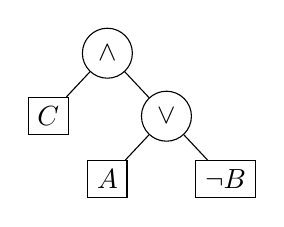
\begin{tikzpicture}[level distance=0.8cm]
          \node[draw,circle] {$\land$}
          child {node[draw,rectangle] {$C$}}
          child {node[draw,circle] {$\lor$}
            child {node[draw,rectangle] {$A$}}
            child {node[draw,rectangle] {$\neg B$}
            }
          };
        \end{tikzpicture}
        \caption{NNF}
      \end{figure}
      \vspace{-1em}
      \begin{figure}
      \centering
        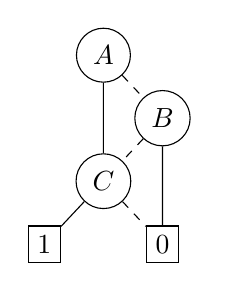
\begin{tikzpicture}[level distance=0.8cm]
          \node[draw,circle] (A) {$A$}
          child {edge from parent[draw=none]}
          child {node[draw,circle] (B) {$B$} edge from parent[dashed]
            child {node[draw,circle,solid] (C) {$C$} edge from parent[dashed]
              child {node[draw,rectangle,solid] {$1$} edge from parent[solid]}
              child {node[draw,rectangle,solid] (0) {$0$}}
            }
            child {edge from parent[draw=none]}
          };
          \draw (A) -- (C);
          \draw (B) -- (0);
        \end{tikzpicture}
        \caption{BDD}
      \end{figure}
    \end{column}
    \begin{column}{0.33\textwidth}
      \begin{figure}
        \centering
        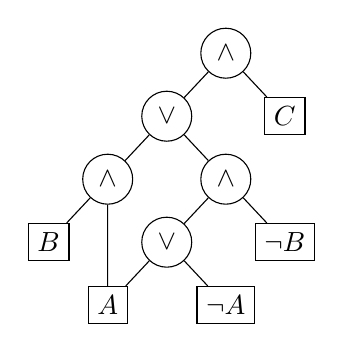
\begin{tikzpicture}[level distance=0.8cm]
          \node[draw,circle] {$\land$}
          child {node[draw,circle] {$\lor$}
            child {node[draw,circle] (parent) {$\land$}
              child {node[draw,rectangle] {$B$}}
              child {edge from parent[draw=none]}
            }
            child {node[draw,circle] {$\land$}
              child {node[draw,circle] {$\lor$}
                child {node[draw,rectangle] (A) {$A$}}
                child {node[draw,rectangle] {$\neg A$}}
              }
              child {node[draw,rectangle] {$\neg B$}}
            }
          }
          child {node[draw,rectangle] {$C$}};
          \draw (parent) -- (A);
        \end{tikzpicture}
        \caption{d-DNNF}
      \end{figure}
    \end{column}
    \begin{column}{0.33\textwidth}
      \begin{figure}
        \centering
        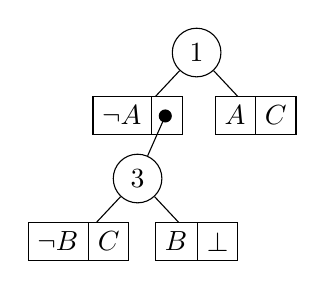
\begin{tikzpicture}[level distance=0.8cm]
          \tikzset{
            mysplit/.style={
              draw,
              rectangle,
              rectangle split,
              rectangle split horizontal,
              rectangle split parts=2
            }
          }
          \node[draw,circle] {$1$}
          child {node[mysplit] (bullet) {
              \nodepart{one} $\neg A$
              \nodepart{two}
            }
            child {node[draw,circle] (3) {$3$} edge from parent[draw=none]
              child {node[mysplit] {
                  \nodepart{one} $\neg B$
                  \nodepart{two} $C$
                }
              }
              child {node[mysplit] {
                  \nodepart{one} $B$
                  \nodepart{two} $\bot$
                }
              }
            }
          }
          child {node[mysplit] {
              \nodepart{one} $A$
              \nodepart{two} $C$
            }};
          \draw[*-] let \p1 = (bullet.two), \p2 = (bullet.center) in ({\x1 + 2.5},{\y2 + 2}) -- (3);
        \end{tikzpicture}
        \caption{SDD}
      \end{figure}
%     \vspace{-2em}
      % \begin{figure}
      % \centering
      % \begin{tikzpicture}[level distance=0.8cm]
      %   \node[draw,circle] {$1$}
      %   child {node[draw,circle] {$0$}
      %     child {node[draw,rectangle] {$A$}}
      %   }
      %   child {node[draw,circle] {$3$}
      %     child {node[draw,circle] {$2$}
      %       child {node[draw,rectangle] {$B$}}
      %     }
      %     child {node[draw,circle] {$4$}
      %       child {node[draw,rectangle] {$C$}}
      %     }
      %   };
      % \end{tikzpicture}
      % \caption{vtree}
      % \end{figure}
    \end{column}
  \end{columns}
\end{frame}

\begin{frame}{Properties of Programs vs. Inference Algorithms}
  \begin{alignat*}{2}
  &\text{Facts:} \quad
  &&\textcolor{predicate}{\mathtt{friend}}(\textcolor{constant}{\mathit{timothy}},
  \textcolor{constant}{\mathit{michelle}}). \\
  &\text{Rules:} \quad &&\textcolor{probability}{0.2} \prob
  \textcolor{predicate}{\mathtt{stress}}(\textcolor{variable}{\mathsf{P}}) \ifff
  \textcolor{predicate}{\mathtt{person}}(\textcolor{variable}{\mathsf{P}}).
  \end{alignat*}
  \centering
  % Created by tikzDevice version 0.12.3 on 2020-07-22 15:14:14
% !TEX encoding = UTF-8 Unicode
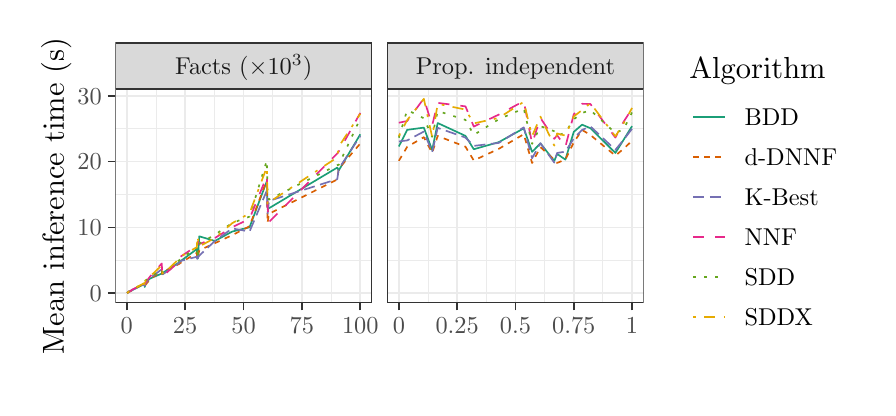
\begin{tikzpicture}[x=1pt,y=1pt]
\definecolor{fillColor}{RGB}{255,255,255}
\path[use as bounding box,fill=fillColor,fill opacity=0.00] (0,0) rectangle (303.53,130.09);
\begin{scope}
\path[clip] (  0.00,  0.00) rectangle (303.53,130.09);
\definecolor{drawColor}{RGB}{255,255,255}
\definecolor{fillColor}{RGB}{255,255,255}

\path[draw=drawColor,line width= 0.6pt,line join=round,line cap=round,fill=fillColor] (  0.00,  0.00) rectangle (303.53,130.09);
\end{scope}
\begin{scope}
\path[clip] ( 31.71, 30.69) rectangle (124.41,108.01);
\definecolor{fillColor}{RGB}{255,255,255}

\path[fill=fillColor] ( 31.71, 30.69) rectangle (124.41,108.01);
\definecolor{drawColor}{gray}{0.92}

\path[draw=drawColor,line width= 0.3pt,line join=round] ( 31.71, 46.03) --
	(124.41, 46.03);

\path[draw=drawColor,line width= 0.3pt,line join=round] ( 31.71, 69.81) --
	(124.41, 69.81);

\path[draw=drawColor,line width= 0.3pt,line join=round] ( 31.71, 93.59) --
	(124.41, 93.59);

\path[draw=drawColor,line width= 0.3pt,line join=round] ( 46.35, 30.69) --
	( 46.35,108.01);

\path[draw=drawColor,line width= 0.3pt,line join=round] ( 67.45, 30.69) --
	( 67.45,108.01);

\path[draw=drawColor,line width= 0.3pt,line join=round] ( 88.54, 30.69) --
	( 88.54,108.01);

\path[draw=drawColor,line width= 0.3pt,line join=round] (109.64, 30.69) --
	(109.64,108.01);

\path[draw=drawColor,line width= 0.6pt,line join=round] ( 31.71, 34.14) --
	(124.41, 34.14);

\path[draw=drawColor,line width= 0.6pt,line join=round] ( 31.71, 57.92) --
	(124.41, 57.92);

\path[draw=drawColor,line width= 0.6pt,line join=round] ( 31.71, 81.70) --
	(124.41, 81.70);

\path[draw=drawColor,line width= 0.6pt,line join=round] ( 31.71,105.48) --
	(124.41,105.48);

\path[draw=drawColor,line width= 0.6pt,line join=round] ( 35.80, 30.69) --
	( 35.80,108.01);

\path[draw=drawColor,line width= 0.6pt,line join=round] ( 56.90, 30.69) --
	( 56.90,108.01);

\path[draw=drawColor,line width= 0.6pt,line join=round] ( 78.00, 30.69) --
	( 78.00,108.01);

\path[draw=drawColor,line width= 0.6pt,line join=round] ( 99.09, 30.69) --
	( 99.09,108.01);

\path[draw=drawColor,line width= 0.6pt,line join=round] (120.19, 30.69) --
	(120.19,108.01);
\definecolor{drawColor}{RGB}{27,158,119}

\path[draw=drawColor,line width= 0.6pt,line join=round] ( 35.93, 34.22) --
	( 36.05, 34.28) --
	( 36.31, 34.45) --
	( 36.64, 34.74) --
	( 36.81, 34.74) --
	( 37.82, 35.27) --
	( 42.19, 37.45) --
	( 42.32, 36.38) --
	( 42.57, 37.84) --
	( 44.24, 39.46) --
	( 48.46, 41.24) --
	( 48.58, 41.31) --
	( 48.84, 41.51) --
	( 54.85, 45.33) --
	( 55.10, 45.62) --
	( 61.12, 50.08) --
	( 61.24, 47.64) --
	( 61.37, 50.15) --
	( 61.50, 46.59) --
	( 62.00, 54.70) --
	( 67.64, 53.02) --
	( 73.90, 56.41) --
	( 80.17, 57.95) --
	( 86.43, 74.63) --
	( 86.69, 65.78) --
	( 87.19, 64.84) --
	(111.88, 79.54) --
	(112.39, 78.48) --
	(120.19, 91.54);
\definecolor{drawColor}{RGB}{217,95,2}

\path[draw=drawColor,line width= 0.6pt,dash pattern=on 2pt off 2pt ,line join=round] ( 35.93, 34.20) --
	( 36.05, 34.26) --
	( 36.31, 34.41) --
	( 36.64, 34.70) --
	( 36.81, 34.68) --
	( 37.82, 35.23) --
	( 42.19, 37.74) --
	( 42.32, 37.05) --
	( 42.57, 37.14) --
	( 44.24, 39.19) --
	( 48.46, 42.35) --
	( 48.58, 40.98) --
	( 48.84, 41.86) --
	( 54.85, 44.75) --
	( 55.10, 45.01) --
	( 61.12, 48.70) --
	( 61.24, 46.51) --
	( 61.37, 47.05) --
	( 61.50, 47.32) --
	( 62.00, 49.64) --
	( 67.64, 52.22) --
	( 73.90, 55.11) --
	( 80.17, 58.33) --
	( 86.43, 75.16) --
	( 86.69, 59.59) --
	( 87.19, 62.82) --
	(111.88, 75.24) --
	(112.39, 79.11) --
	(120.19, 88.23);
\definecolor{drawColor}{RGB}{117,112,179}

\path[draw=drawColor,line width= 0.6pt,dash pattern=on 4pt off 2pt ,line join=round] ( 35.93, 34.22) --
	( 36.05, 34.33) --
	( 36.31, 34.49) --
	( 36.64, 34.77) --
	( 36.81, 34.77) --
	( 37.82, 35.37) --
	( 42.19, 37.40) --
	( 42.32, 36.84) --
	( 42.57, 37.68) --
	( 44.24, 39.58) --
	( 48.46, 42.81) --
	( 48.58, 41.77) --
	( 48.84, 40.98) --
	( 54.85, 45.16) --
	( 55.10, 45.74) --
	( 61.12, 47.31) --
	( 61.24, 46.52) --
	( 61.37, 48.59) --
	( 61.50, 46.96) --
	( 62.00, 47.72) --
	( 67.64, 52.99) --
	( 73.90, 57.55) --
	( 80.17, 56.42) --
	( 86.43, 71.23) --
	( 86.69, 62.93) --
	( 87.19, 67.49) --
	(111.88, 75.36) --
	(112.39, 79.09) --
	(120.19, 90.92);
\definecolor{drawColor}{RGB}{231,41,138}

\path[draw=drawColor,line width= 0.6pt,dash pattern=on 4pt off 4pt ,line join=round] ( 35.93, 34.22) --
	( 36.05, 34.29) --
	( 36.31, 34.48) --
	( 36.64, 34.79) --
	( 36.81, 34.74) --
	( 37.82, 35.45) --
	( 42.19, 37.64) --
	( 42.32, 37.18) --
	( 42.57, 37.98) --
	( 44.24, 40.20) --
	( 48.46, 44.88) --
	( 48.58, 42.06) --
	( 48.84, 40.35) --
	( 54.85, 45.65) --
	( 55.10, 47.25) --
	( 61.12, 51.25) --
	( 61.24, 51.16) --
	( 61.37, 51.25) --
	( 61.50, 52.79) --
	( 62.00, 51.87) --
	( 67.64, 54.08) --
	( 73.90, 57.97) --
	( 80.17, 61.03) --
	( 86.43, 76.47) --
	( 86.69, 65.20) --
	( 87.19, 59.83) --
	(111.88, 84.66) --
	(112.39, 85.31) --
	(120.19, 99.29);
\definecolor{drawColor}{RGB}{102,166,30}

\path[draw=drawColor,line width= 0.6pt,dash pattern=on 1pt off 3pt ,line join=round] ( 35.93, 34.24) --
	( 36.05, 34.31) --
	( 36.31, 34.48) --
	( 36.64, 34.81) --
	( 36.81, 34.77) --
	( 37.82, 35.45) --
	( 42.19, 37.88) --
	( 42.32, 38.54) --
	( 42.57, 38.69) --
	( 44.24, 39.95) --
	( 48.46, 42.70) --
	( 48.58, 41.93) --
	( 48.84, 41.20) --
	( 54.85, 46.14) --
	( 55.10, 46.43) --
	( 61.12, 50.70) --
	( 61.24, 47.87) --
	( 61.37, 50.28) --
	( 61.50, 47.98) --
	( 62.00, 52.07) --
	( 67.64, 55.24) --
	( 73.90, 59.51) --
	( 80.17, 61.81) --
	( 86.43, 82.15) --
	( 86.69, 68.77) --
	( 87.19, 67.98) --
	(111.88, 80.43) --
	(112.39, 80.51) --
	(120.19, 97.30);
\definecolor{drawColor}{RGB}{230,171,2}

\path[draw=drawColor,line width= 0.6pt,dash pattern=on 1pt off 3pt on 4pt off 3pt ,line join=round] ( 35.93, 34.20) --
	( 36.05, 34.32) --
	( 36.31, 34.47) --
	( 36.64, 34.80) --
	( 36.81, 34.78) --
	( 37.82, 35.44) --
	( 42.19, 37.83) --
	( 42.32, 36.07) --
	( 42.57, 38.73) --
	( 44.24, 40.20) --
	( 48.46, 44.23) --
	( 48.58, 43.29) --
	( 48.84, 40.97) --
	( 54.85, 46.70) --
	( 55.10, 47.28) --
	( 61.12, 50.76) --
	( 61.24, 52.81) --
	( 61.37, 51.86) --
	( 61.50, 53.84) --
	( 62.00, 51.03) --
	( 67.64, 54.08) --
	( 73.90, 59.44) --
	( 80.17, 63.01) --
	( 86.43, 79.72) --
	( 86.69, 66.18) --
	( 87.19, 66.97) --
	(111.88, 83.22) --
	(112.39, 87.08) --
	(120.19, 98.99);
\definecolor{drawColor}{gray}{0.20}

\path[draw=drawColor,line width= 0.6pt,line join=round,line cap=round] ( 31.71, 30.69) rectangle (124.41,108.01);
\end{scope}
\begin{scope}
\path[clip] (129.91, 30.69) rectangle (222.60,108.01);
\definecolor{fillColor}{RGB}{255,255,255}

\path[fill=fillColor] (129.91, 30.69) rectangle (222.60,108.01);
\definecolor{drawColor}{gray}{0.92}

\path[draw=drawColor,line width= 0.3pt,line join=round] (129.91, 46.03) --
	(222.60, 46.03);

\path[draw=drawColor,line width= 0.3pt,line join=round] (129.91, 69.81) --
	(222.60, 69.81);

\path[draw=drawColor,line width= 0.3pt,line join=round] (129.91, 93.59) --
	(222.60, 93.59);

\path[draw=drawColor,line width= 0.3pt,line join=round] (144.65, 30.69) --
	(144.65,108.01);

\path[draw=drawColor,line width= 0.3pt,line join=round] (165.72, 30.69) --
	(165.72,108.01);

\path[draw=drawColor,line width= 0.3pt,line join=round] (186.79, 30.69) --
	(186.79,108.01);

\path[draw=drawColor,line width= 0.3pt,line join=round] (207.85, 30.69) --
	(207.85,108.01);

\path[draw=drawColor,line width= 0.6pt,line join=round] (129.91, 34.14) --
	(222.60, 34.14);

\path[draw=drawColor,line width= 0.6pt,line join=round] (129.91, 57.92) --
	(222.60, 57.92);

\path[draw=drawColor,line width= 0.6pt,line join=round] (129.91, 81.70) --
	(222.60, 81.70);

\path[draw=drawColor,line width= 0.6pt,line join=round] (129.91,105.48) --
	(222.60,105.48);

\path[draw=drawColor,line width= 0.6pt,line join=round] (134.12, 30.69) --
	(134.12,108.01);

\path[draw=drawColor,line width= 0.6pt,line join=round] (155.19, 30.69) --
	(155.19,108.01);

\path[draw=drawColor,line width= 0.6pt,line join=round] (176.25, 30.69) --
	(176.25,108.01);

\path[draw=drawColor,line width= 0.6pt,line join=round] (197.32, 30.69) --
	(197.32,108.01);

\path[draw=drawColor,line width= 0.6pt,line join=round] (218.39, 30.69) --
	(218.39,108.01);
\definecolor{drawColor}{RGB}{27,158,119}

\path[draw=drawColor,line width= 0.6pt,line join=round] (134.12, 87.17) --
	(137.13, 93.17) --
	(143.15, 93.97) --
	(146.16, 85.86) --
	(148.16, 95.63) --
	(158.20, 90.99) --
	(161.20, 86.16) --
	(170.23, 88.72) --
	(179.26, 93.71) --
	(182.27, 85.21) --
	(185.28, 88.26) --
	(190.30, 81.94) --
	(191.30, 84.46) --
	(194.31, 82.43) --
	(197.32, 92.42) --
	(200.33, 95.04) --
	(203.34, 93.76) --
	(212.37, 84.82) --
	(215.38, 89.64) --
	(218.39, 94.51);
\definecolor{drawColor}{RGB}{217,95,2}

\path[draw=drawColor,line width= 0.6pt,dash pattern=on 2pt off 2pt ,line join=round] (134.12, 81.98) --
	(137.13, 87.03) --
	(143.15, 90.51) --
	(146.16, 84.86) --
	(148.16, 90.95) --
	(158.20, 87.07) --
	(161.20, 82.10) --
	(170.23, 86.31) --
	(179.26, 91.58) --
	(182.27, 81.17) --
	(185.28, 86.92) --
	(190.30, 82.36) --
	(191.30, 81.20) --
	(194.31, 82.46) --
	(197.32, 88.61) --
	(200.33, 93.14) --
	(203.34, 91.31) --
	(212.37, 83.85) --
	(215.38, 86.37) --
	(218.39, 89.25);
\definecolor{drawColor}{RGB}{117,112,179}

\path[draw=drawColor,line width= 0.6pt,dash pattern=on 4pt off 2pt ,line join=round] (134.12, 88.97) --
	(137.13, 89.35) --
	(143.15, 92.54) --
	(146.16, 85.10) --
	(148.16, 93.89) --
	(158.20, 90.38) --
	(161.20, 87.37) --
	(170.23, 88.45) --
	(179.26, 94.07) --
	(182.27, 82.90) --
	(185.28, 88.35) --
	(190.30, 81.32) --
	(191.30, 84.81) --
	(194.31, 85.30) --
	(197.32, 90.02) --
	(200.33, 93.14) --
	(203.34, 94.41) --
	(212.37, 85.94) --
	(215.38, 89.62) --
	(218.39, 93.56);
\definecolor{drawColor}{RGB}{231,41,138}

\path[draw=drawColor,line width= 0.6pt,dash pattern=on 4pt off 4pt ,line join=round] (134.12, 95.74) --
	(137.13, 96.35) --
	(143.15,104.50) --
	(146.16, 94.79) --
	(148.16,102.91) --
	(158.20,101.65) --
	(161.20, 94.35) --
	(170.23, 98.68) --
	(179.26,103.55) --
	(182.27, 88.20) --
	(185.28, 97.47) --
	(190.30, 89.92) --
	(191.30, 91.22) --
	(194.31, 87.06) --
	(197.32, 98.75) --
	(200.33,102.58) --
	(203.34,102.50) --
	(212.37, 90.37) --
	(215.38, 96.15) --
	(218.39,100.82);
\definecolor{drawColor}{RGB}{102,166,30}

\path[draw=drawColor,line width= 0.6pt,dash pattern=on 1pt off 3pt ,line join=round] (134.12, 90.34) --
	(137.13,100.33) --
	(143.15, 97.34) --
	(146.16, 90.63) --
	(148.16, 99.99) --
	(158.20, 96.75) --
	(161.20, 91.32) --
	(170.23, 97.00) --
	(179.26,100.90) --
	(182.27, 88.11) --
	(185.28, 94.51) --
	(190.30, 92.66) --
	(191.30, 90.99) --
	(194.31, 92.19) --
	(197.32, 96.98) --
	(200.33, 99.26) --
	(203.34,100.29) --
	(212.37, 92.01) --
	(215.38, 93.41) --
	(218.39, 99.52);
\definecolor{drawColor}{RGB}{230,171,2}

\path[draw=drawColor,line width= 0.6pt,dash pattern=on 1pt off 3pt on 4pt off 3pt ,line join=round] (134.12, 90.96) --
	(137.13, 96.67) --
	(143.15,104.39) --
	(146.16, 90.59) --
	(148.16,102.58) --
	(158.20,100.48) --
	(161.20, 95.50) --
	(170.23, 97.48) --
	(179.26,103.31) --
	(182.27, 90.87) --
	(185.28, 97.96) --
	(190.30, 87.48) --
	(191.30, 91.85) --
	(194.31, 91.08) --
	(197.32, 98.02) --
	(200.33,100.29) --
	(203.34,102.81) --
	(212.37, 90.81) --
	(215.38, 95.58) --
	(218.39,101.07);
\definecolor{drawColor}{gray}{0.20}

\path[draw=drawColor,line width= 0.6pt,line join=round,line cap=round] (129.91, 30.69) rectangle (222.60,108.01);
\end{scope}
\begin{scope}
\path[clip] ( 31.71,108.01) rectangle (124.41,124.59);
\definecolor{drawColor}{gray}{0.20}
\definecolor{fillColor}{gray}{0.85}

\path[draw=drawColor,line width= 0.6pt,line join=round,line cap=round,fill=fillColor] ( 31.71,108.01) rectangle (124.41,124.59);
\definecolor{drawColor}{gray}{0.10}

\node[text=drawColor,anchor=base,inner sep=0pt, outer sep=0pt, scale=  0.88] at ( 78.06,113.27) {Facts ($\times 10^3$)};
\end{scope}
\begin{scope}
\path[clip] (129.91,108.01) rectangle (222.60,124.59);
\definecolor{drawColor}{gray}{0.20}
\definecolor{fillColor}{gray}{0.85}

\path[draw=drawColor,line width= 0.6pt,line join=round,line cap=round,fill=fillColor] (129.91,108.01) rectangle (222.60,124.59);
\definecolor{drawColor}{gray}{0.10}

\node[text=drawColor,anchor=base,inner sep=0pt, outer sep=0pt, scale=  0.88] at (176.25,113.27) {Prop. independent};
\end{scope}
\begin{scope}
\path[clip] (  0.00,  0.00) rectangle (303.53,130.09);
\definecolor{drawColor}{gray}{0.20}

\path[draw=drawColor,line width= 0.6pt,line join=round] ( 35.80, 27.94) --
	( 35.80, 30.69);

\path[draw=drawColor,line width= 0.6pt,line join=round] ( 56.90, 27.94) --
	( 56.90, 30.69);

\path[draw=drawColor,line width= 0.6pt,line join=round] ( 78.00, 27.94) --
	( 78.00, 30.69);

\path[draw=drawColor,line width= 0.6pt,line join=round] ( 99.09, 27.94) --
	( 99.09, 30.69);

\path[draw=drawColor,line width= 0.6pt,line join=round] (120.19, 27.94) --
	(120.19, 30.69);
\end{scope}
\begin{scope}
\path[clip] (  0.00,  0.00) rectangle (303.53,130.09);
\definecolor{drawColor}{gray}{0.30}

\node[text=drawColor,anchor=base,inner sep=0pt, outer sep=0pt, scale=  0.88] at ( 35.80, 19.68) {0};

\node[text=drawColor,anchor=base,inner sep=0pt, outer sep=0pt, scale=  0.88] at ( 56.90, 19.68) {25};

\node[text=drawColor,anchor=base,inner sep=0pt, outer sep=0pt, scale=  0.88] at ( 78.00, 19.68) {50};

\node[text=drawColor,anchor=base,inner sep=0pt, outer sep=0pt, scale=  0.88] at ( 99.09, 19.68) {75};

\node[text=drawColor,anchor=base,inner sep=0pt, outer sep=0pt, scale=  0.88] at (120.19, 19.68) {100};
\end{scope}
\begin{scope}
\path[clip] (  0.00,  0.00) rectangle (303.53,130.09);
\definecolor{drawColor}{gray}{0.20}

\path[draw=drawColor,line width= 0.6pt,line join=round] (134.12, 27.94) --
	(134.12, 30.69);

\path[draw=drawColor,line width= 0.6pt,line join=round] (155.19, 27.94) --
	(155.19, 30.69);

\path[draw=drawColor,line width= 0.6pt,line join=round] (176.25, 27.94) --
	(176.25, 30.69);

\path[draw=drawColor,line width= 0.6pt,line join=round] (197.32, 27.94) --
	(197.32, 30.69);

\path[draw=drawColor,line width= 0.6pt,line join=round] (218.39, 27.94) --
	(218.39, 30.69);
\end{scope}
\begin{scope}
\path[clip] (  0.00,  0.00) rectangle (303.53,130.09);
\definecolor{drawColor}{gray}{0.30}

\node[text=drawColor,anchor=base,inner sep=0pt, outer sep=0pt, scale=  0.88] at (134.12, 19.68) {0};

\node[text=drawColor,anchor=base,inner sep=0pt, outer sep=0pt, scale=  0.88] at (155.19, 19.68) {0.25};

\node[text=drawColor,anchor=base,inner sep=0pt, outer sep=0pt, scale=  0.88] at (176.25, 19.68) {0.5};

\node[text=drawColor,anchor=base,inner sep=0pt, outer sep=0pt, scale=  0.88] at (197.32, 19.68) {0.75};

\node[text=drawColor,anchor=base,inner sep=0pt, outer sep=0pt, scale=  0.88] at (218.39, 19.68) {1};
\end{scope}
\begin{scope}
\path[clip] (  0.00,  0.00) rectangle (303.53,130.09);
\definecolor{drawColor}{gray}{0.30}

\node[text=drawColor,anchor=base east,inner sep=0pt, outer sep=0pt, scale=  0.88] at ( 26.76, 31.11) {0};

\node[text=drawColor,anchor=base east,inner sep=0pt, outer sep=0pt, scale=  0.88] at ( 26.76, 54.89) {10};

\node[text=drawColor,anchor=base east,inner sep=0pt, outer sep=0pt, scale=  0.88] at ( 26.76, 78.67) {20};

\node[text=drawColor,anchor=base east,inner sep=0pt, outer sep=0pt, scale=  0.88] at ( 26.76,102.45) {30};
\end{scope}
\begin{scope}
\path[clip] (  0.00,  0.00) rectangle (303.53,130.09);
\definecolor{drawColor}{gray}{0.20}

\path[draw=drawColor,line width= 0.6pt,line join=round] ( 28.96, 34.14) --
	( 31.71, 34.14);

\path[draw=drawColor,line width= 0.6pt,line join=round] ( 28.96, 57.92) --
	( 31.71, 57.92);

\path[draw=drawColor,line width= 0.6pt,line join=round] ( 28.96, 81.70) --
	( 31.71, 81.70);

\path[draw=drawColor,line width= 0.6pt,line join=round] ( 28.96,105.48) --
	( 31.71,105.48);
\end{scope}
\begin{scope}
\path[clip] (  0.00,  0.00) rectangle (303.53,130.09);
\definecolor{drawColor}{RGB}{0,0,0}

\node[text=drawColor,rotate= 90.00,anchor=base,inner sep=0pt, outer sep=0pt, scale=  1.10] at ( 13.08, 69.35) {Mean inference time (s)};
\end{scope}
\begin{scope}
\path[clip] (  0.00,  0.00) rectangle (303.53,130.09);
\definecolor{fillColor}{RGB}{255,255,255}

\path[fill=fillColor] (233.60, 12.88) rectangle (298.03,125.82);
\end{scope}
\begin{scope}
\path[clip] (  0.00,  0.00) rectangle (303.53,130.09);
\definecolor{drawColor}{RGB}{0,0,0}

\node[text=drawColor,anchor=base west,inner sep=0pt, outer sep=0pt, scale=  1.10] at (239.10,111.67) {Algorithm};
\end{scope}
\begin{scope}
\path[clip] (  0.00,  0.00) rectangle (303.53,130.09);
\definecolor{fillColor}{RGB}{255,255,255}

\path[fill=fillColor] (239.10, 90.65) rectangle (253.55,105.10);
\end{scope}
\begin{scope}
\path[clip] (  0.00,  0.00) rectangle (303.53,130.09);
\definecolor{drawColor}{RGB}{27,158,119}

\path[draw=drawColor,line width= 0.6pt,line join=round] (240.54, 97.88) -- (252.11, 97.88);
\end{scope}
\begin{scope}
\path[clip] (  0.00,  0.00) rectangle (303.53,130.09);
\definecolor{fillColor}{RGB}{255,255,255}

\path[fill=fillColor] (239.10, 76.20) rectangle (253.55, 90.65);
\end{scope}
\begin{scope}
\path[clip] (  0.00,  0.00) rectangle (303.53,130.09);
\definecolor{drawColor}{RGB}{217,95,2}

\path[draw=drawColor,line width= 0.6pt,dash pattern=on 2pt off 2pt ,line join=round] (240.54, 83.42) -- (252.11, 83.42);
\end{scope}
\begin{scope}
\path[clip] (  0.00,  0.00) rectangle (303.53,130.09);
\definecolor{fillColor}{RGB}{255,255,255}

\path[fill=fillColor] (239.10, 61.74) rectangle (253.55, 76.20);
\end{scope}
\begin{scope}
\path[clip] (  0.00,  0.00) rectangle (303.53,130.09);
\definecolor{drawColor}{RGB}{117,112,179}

\path[draw=drawColor,line width= 0.6pt,dash pattern=on 4pt off 2pt ,line join=round] (240.54, 68.97) -- (252.11, 68.97);
\end{scope}
\begin{scope}
\path[clip] (  0.00,  0.00) rectangle (303.53,130.09);
\definecolor{fillColor}{RGB}{255,255,255}

\path[fill=fillColor] (239.10, 47.29) rectangle (253.55, 61.74);
\end{scope}
\begin{scope}
\path[clip] (  0.00,  0.00) rectangle (303.53,130.09);
\definecolor{drawColor}{RGB}{231,41,138}

\path[draw=drawColor,line width= 0.6pt,dash pattern=on 4pt off 4pt ,line join=round] (240.54, 54.52) -- (252.11, 54.52);
\end{scope}
\begin{scope}
\path[clip] (  0.00,  0.00) rectangle (303.53,130.09);
\definecolor{fillColor}{RGB}{255,255,255}

\path[fill=fillColor] (239.10, 32.83) rectangle (253.55, 47.29);
\end{scope}
\begin{scope}
\path[clip] (  0.00,  0.00) rectangle (303.53,130.09);
\definecolor{drawColor}{RGB}{102,166,30}

\path[draw=drawColor,line width= 0.6pt,dash pattern=on 1pt off 3pt ,line join=round] (240.54, 40.06) -- (252.11, 40.06);
\end{scope}
\begin{scope}
\path[clip] (  0.00,  0.00) rectangle (303.53,130.09);
\definecolor{fillColor}{RGB}{255,255,255}

\path[fill=fillColor] (239.10, 18.38) rectangle (253.55, 32.83);
\end{scope}
\begin{scope}
\path[clip] (  0.00,  0.00) rectangle (303.53,130.09);
\definecolor{drawColor}{RGB}{230,171,2}

\path[draw=drawColor,line width= 0.6pt,dash pattern=on 1pt off 3pt on 4pt off 3pt ,line join=round] (240.54, 25.61) -- (252.11, 25.61);
\end{scope}
\begin{scope}
\path[clip] (  0.00,  0.00) rectangle (303.53,130.09);
\definecolor{drawColor}{RGB}{0,0,0}

\node[text=drawColor,anchor=base west,inner sep=0pt, outer sep=0pt, scale=  0.88] at (259.05, 94.85) {BDD};
\end{scope}
\begin{scope}
\path[clip] (  0.00,  0.00) rectangle (303.53,130.09);
\definecolor{drawColor}{RGB}{0,0,0}

\node[text=drawColor,anchor=base west,inner sep=0pt, outer sep=0pt, scale=  0.88] at (259.05, 80.39) {d-DNNF};
\end{scope}
\begin{scope}
\path[clip] (  0.00,  0.00) rectangle (303.53,130.09);
\definecolor{drawColor}{RGB}{0,0,0}

\node[text=drawColor,anchor=base west,inner sep=0pt, outer sep=0pt, scale=  0.88] at (259.05, 65.94) {K-Best};
\end{scope}
\begin{scope}
\path[clip] (  0.00,  0.00) rectangle (303.53,130.09);
\definecolor{drawColor}{RGB}{0,0,0}

\node[text=drawColor,anchor=base west,inner sep=0pt, outer sep=0pt, scale=  0.88] at (259.05, 51.49) {NNF};
\end{scope}
\begin{scope}
\path[clip] (  0.00,  0.00) rectangle (303.53,130.09);
\definecolor{drawColor}{RGB}{0,0,0}

\node[text=drawColor,anchor=base west,inner sep=0pt, outer sep=0pt, scale=  0.88] at (259.05, 37.03) {SDD};
\end{scope}
\begin{scope}
\path[clip] (  0.00,  0.00) rectangle (303.53,130.09);
\definecolor{drawColor}{RGB}{0,0,0}

\node[text=drawColor,anchor=base west,inner sep=0pt, outer sep=0pt, scale=  0.88] at (259.05, 22.58) {SDDX};
\end{scope}
\end{tikzpicture}

\end{frame}

\begin{frame}{Properties of Programs vs. Inference Algorithms}
  \centering
  % Created by tikzDevice version 0.12.3 on 2020-05-14 17:55:45
% !TEX encoding = UTF-8 Unicode
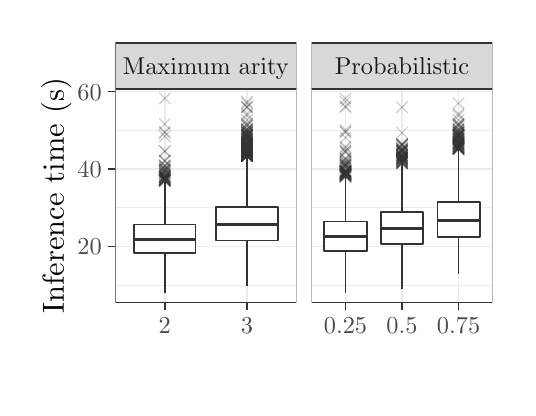
\begin{tikzpicture}[x=1pt,y=1pt]
\definecolor{fillColor}{RGB}{255,255,255}
\path[use as bounding box,fill=fillColor,fill opacity=0.00] (0,0) rectangle (173.45,130.09);
\begin{scope}
\path[clip] (  0.00,  0.00) rectangle (173.45,130.09);
\definecolor{drawColor}{RGB}{255,255,255}
\definecolor{fillColor}{RGB}{255,255,255}

\path[draw=drawColor,line width= 0.6pt,line join=round,line cap=round,fill=fillColor] ( -0.00,  0.00) rectangle (173.45,130.09);
\end{scope}
\begin{scope}
\path[clip] ( 31.71, 30.69) rectangle ( 97.08,108.01);
\definecolor{fillColor}{RGB}{255,255,255}

\path[fill=fillColor] ( 31.71, 30.69) rectangle ( 97.08,108.01);
\definecolor{drawColor}{gray}{0.92}

\path[draw=drawColor,line width= 0.3pt,line join=round] ( 31.71, 36.97) --
	( 97.08, 36.97);

\path[draw=drawColor,line width= 0.3pt,line join=round] ( 31.71, 64.98) --
	( 97.08, 64.98);

\path[draw=drawColor,line width= 0.3pt,line join=round] ( 31.71, 92.98) --
	( 97.08, 92.98);

\path[draw=drawColor,line width= 0.6pt,line join=round] ( 31.71, 50.98) --
	( 97.08, 50.98);

\path[draw=drawColor,line width= 0.6pt,line join=round] ( 31.71, 78.98) --
	( 97.08, 78.98);

\path[draw=drawColor,line width= 0.6pt,line join=round] ( 31.71,106.99) --
	( 97.08,106.99);

\path[draw=drawColor,line width= 0.6pt,line join=round] ( 49.54, 30.69) --
	( 49.54,108.01);

\path[draw=drawColor,line width= 0.6pt,line join=round] ( 79.25, 30.69) --
	( 79.25,108.01);
\definecolor{drawColor}{RGB}{51,51,51}

\path[draw=drawColor,draw opacity=0.25,line width= 0.4pt,line join=round,line cap=round] ( 47.58, 74.50) -- ( 51.50, 78.42);

\path[draw=drawColor,draw opacity=0.25,line width= 0.4pt,line join=round,line cap=round] ( 47.58, 78.42) -- ( 51.50, 74.50);

\path[draw=drawColor,draw opacity=0.25,line width= 0.4pt,line join=round,line cap=round] ( 47.58, 73.55) -- ( 51.50, 77.47);

\path[draw=drawColor,draw opacity=0.25,line width= 0.4pt,line join=round,line cap=round] ( 47.58, 77.47) -- ( 51.50, 73.55);

\path[draw=drawColor,draw opacity=0.25,line width= 0.4pt,line join=round,line cap=round] ( 47.58, 83.41) -- ( 51.50, 87.33);

\path[draw=drawColor,draw opacity=0.25,line width= 0.4pt,line join=round,line cap=round] ( 47.58, 87.33) -- ( 51.50, 83.41);

\path[draw=drawColor,draw opacity=0.25,line width= 0.4pt,line join=round,line cap=round] ( 47.58, 78.42) -- ( 51.50, 82.34);

\path[draw=drawColor,draw opacity=0.25,line width= 0.4pt,line join=round,line cap=round] ( 47.58, 82.34) -- ( 51.50, 78.42);

\path[draw=drawColor,draw opacity=0.25,line width= 0.4pt,line join=round,line cap=round] ( 47.58, 76.11) -- ( 51.50, 80.03);

\path[draw=drawColor,draw opacity=0.25,line width= 0.4pt,line join=round,line cap=round] ( 47.58, 80.03) -- ( 51.50, 76.11);

\path[draw=drawColor,draw opacity=0.25,line width= 0.4pt,line join=round,line cap=round] ( 47.58, 74.48) -- ( 51.50, 78.40);

\path[draw=drawColor,draw opacity=0.25,line width= 0.4pt,line join=round,line cap=round] ( 47.58, 78.40) -- ( 51.50, 74.48);

\path[draw=drawColor,draw opacity=0.25,line width= 0.4pt,line join=round,line cap=round] ( 47.58, 76.90) -- ( 51.50, 80.82);

\path[draw=drawColor,draw opacity=0.25,line width= 0.4pt,line join=round,line cap=round] ( 47.58, 80.82) -- ( 51.50, 76.90);

\path[draw=drawColor,draw opacity=0.25,line width= 0.4pt,line join=round,line cap=round] ( 47.58, 72.95) -- ( 51.50, 76.87);

\path[draw=drawColor,draw opacity=0.25,line width= 0.4pt,line join=round,line cap=round] ( 47.58, 76.87) -- ( 51.50, 72.95);

\path[draw=drawColor,draw opacity=0.25,line width= 0.4pt,line join=round,line cap=round] ( 47.58, 77.09) -- ( 51.50, 81.02);

\path[draw=drawColor,draw opacity=0.25,line width= 0.4pt,line join=round,line cap=round] ( 47.58, 81.02) -- ( 51.50, 77.09);

\path[draw=drawColor,draw opacity=0.25,line width= 0.4pt,line join=round,line cap=round] ( 47.58, 74.11) -- ( 51.50, 78.03);

\path[draw=drawColor,draw opacity=0.25,line width= 0.4pt,line join=round,line cap=round] ( 47.58, 78.03) -- ( 51.50, 74.11);

\path[draw=drawColor,draw opacity=0.25,line width= 0.4pt,line join=round,line cap=round] ( 47.58, 76.69) -- ( 51.50, 80.62);

\path[draw=drawColor,draw opacity=0.25,line width= 0.4pt,line join=round,line cap=round] ( 47.58, 80.62) -- ( 51.50, 76.69);

\path[draw=drawColor,draw opacity=0.25,line width= 0.4pt,line join=round,line cap=round] ( 47.58, 75.42) -- ( 51.50, 79.34);

\path[draw=drawColor,draw opacity=0.25,line width= 0.4pt,line join=round,line cap=round] ( 47.58, 79.34) -- ( 51.50, 75.42);

\path[draw=drawColor,draw opacity=0.25,line width= 0.4pt,line join=round,line cap=round] ( 47.58, 73.74) -- ( 51.50, 77.67);

\path[draw=drawColor,draw opacity=0.25,line width= 0.4pt,line join=round,line cap=round] ( 47.58, 77.67) -- ( 51.50, 73.74);

\path[draw=drawColor,draw opacity=0.25,line width= 0.4pt,line join=round,line cap=round] ( 47.58, 74.11) -- ( 51.50, 78.03);

\path[draw=drawColor,draw opacity=0.25,line width= 0.4pt,line join=round,line cap=round] ( 47.58, 78.03) -- ( 51.50, 74.11);

\path[draw=drawColor,draw opacity=0.25,line width= 0.4pt,line join=round,line cap=round] ( 47.58, 74.03) -- ( 51.50, 77.96);

\path[draw=drawColor,draw opacity=0.25,line width= 0.4pt,line join=round,line cap=round] ( 47.58, 77.96) -- ( 51.50, 74.03);

\path[draw=drawColor,draw opacity=0.25,line width= 0.4pt,line join=round,line cap=round] ( 47.58, 76.80) -- ( 51.50, 80.72);

\path[draw=drawColor,draw opacity=0.25,line width= 0.4pt,line join=round,line cap=round] ( 47.58, 80.72) -- ( 51.50, 76.80);

\path[draw=drawColor,draw opacity=0.25,line width= 0.4pt,line join=round,line cap=round] ( 47.58, 74.58) -- ( 51.50, 78.50);

\path[draw=drawColor,draw opacity=0.25,line width= 0.4pt,line join=round,line cap=round] ( 47.58, 78.50) -- ( 51.50, 74.58);

\path[draw=drawColor,draw opacity=0.25,line width= 0.4pt,line join=round,line cap=round] ( 47.58, 73.04) -- ( 51.50, 76.96);

\path[draw=drawColor,draw opacity=0.25,line width= 0.4pt,line join=round,line cap=round] ( 47.58, 76.96) -- ( 51.50, 73.04);

\path[draw=drawColor,draw opacity=0.25,line width= 0.4pt,line join=round,line cap=round] ( 47.58, 74.11) -- ( 51.50, 78.03);

\path[draw=drawColor,draw opacity=0.25,line width= 0.4pt,line join=round,line cap=round] ( 47.58, 78.03) -- ( 51.50, 74.11);

\path[draw=drawColor,draw opacity=0.25,line width= 0.4pt,line join=round,line cap=round] ( 47.58, 74.24) -- ( 51.50, 78.16);

\path[draw=drawColor,draw opacity=0.25,line width= 0.4pt,line join=round,line cap=round] ( 47.58, 78.16) -- ( 51.50, 74.24);

\path[draw=drawColor,draw opacity=0.25,line width= 0.4pt,line join=round,line cap=round] ( 47.58, 73.75) -- ( 51.50, 77.68);

\path[draw=drawColor,draw opacity=0.25,line width= 0.4pt,line join=round,line cap=round] ( 47.58, 77.68) -- ( 51.50, 73.75);

\path[draw=drawColor,draw opacity=0.25,line width= 0.4pt,line join=round,line cap=round] ( 47.58, 73.33) -- ( 51.50, 77.25);

\path[draw=drawColor,draw opacity=0.25,line width= 0.4pt,line join=round,line cap=round] ( 47.58, 77.25) -- ( 51.50, 73.33);

\path[draw=drawColor,draw opacity=0.25,line width= 0.4pt,line join=round,line cap=round] ( 47.58, 75.34) -- ( 51.50, 79.26);

\path[draw=drawColor,draw opacity=0.25,line width= 0.4pt,line join=round,line cap=round] ( 47.58, 79.26) -- ( 51.50, 75.34);

\path[draw=drawColor,draw opacity=0.25,line width= 0.4pt,line join=round,line cap=round] ( 47.58, 75.66) -- ( 51.50, 79.58);

\path[draw=drawColor,draw opacity=0.25,line width= 0.4pt,line join=round,line cap=round] ( 47.58, 79.58) -- ( 51.50, 75.66);

\path[draw=drawColor,draw opacity=0.25,line width= 0.4pt,line join=round,line cap=round] ( 47.58, 72.71) -- ( 51.50, 76.63);

\path[draw=drawColor,draw opacity=0.25,line width= 0.4pt,line join=round,line cap=round] ( 47.58, 76.63) -- ( 51.50, 72.71);

\path[draw=drawColor,draw opacity=0.25,line width= 0.4pt,line join=round,line cap=round] ( 47.58, 77.76) -- ( 51.50, 81.69);

\path[draw=drawColor,draw opacity=0.25,line width= 0.4pt,line join=round,line cap=round] ( 47.58, 81.69) -- ( 51.50, 77.76);

\path[draw=drawColor,draw opacity=0.25,line width= 0.4pt,line join=round,line cap=round] ( 47.58, 76.89) -- ( 51.50, 80.82);

\path[draw=drawColor,draw opacity=0.25,line width= 0.4pt,line join=round,line cap=round] ( 47.58, 80.82) -- ( 51.50, 76.89);

\path[draw=drawColor,draw opacity=0.25,line width= 0.4pt,line join=round,line cap=round] ( 47.58, 74.43) -- ( 51.50, 78.36);

\path[draw=drawColor,draw opacity=0.25,line width= 0.4pt,line join=round,line cap=round] ( 47.58, 78.36) -- ( 51.50, 74.43);

\path[draw=drawColor,draw opacity=0.25,line width= 0.4pt,line join=round,line cap=round] ( 47.58, 73.36) -- ( 51.50, 77.29);

\path[draw=drawColor,draw opacity=0.25,line width= 0.4pt,line join=round,line cap=round] ( 47.58, 77.29) -- ( 51.50, 73.36);

\path[draw=drawColor,draw opacity=0.25,line width= 0.4pt,line join=round,line cap=round] ( 47.58, 73.28) -- ( 51.50, 77.20);

\path[draw=drawColor,draw opacity=0.25,line width= 0.4pt,line join=round,line cap=round] ( 47.58, 77.20) -- ( 51.50, 73.28);

\path[draw=drawColor,draw opacity=0.25,line width= 0.4pt,line join=round,line cap=round] ( 47.58, 73.81) -- ( 51.50, 77.73);

\path[draw=drawColor,draw opacity=0.25,line width= 0.4pt,line join=round,line cap=round] ( 47.58, 77.73) -- ( 51.50, 73.81);

\path[draw=drawColor,draw opacity=0.25,line width= 0.4pt,line join=round,line cap=round] ( 47.58, 76.10) -- ( 51.50, 80.03);

\path[draw=drawColor,draw opacity=0.25,line width= 0.4pt,line join=round,line cap=round] ( 47.58, 80.03) -- ( 51.50, 76.10);

\path[draw=drawColor,draw opacity=0.25,line width= 0.4pt,line join=round,line cap=round] ( 47.58, 75.24) -- ( 51.50, 79.16);

\path[draw=drawColor,draw opacity=0.25,line width= 0.4pt,line join=round,line cap=round] ( 47.58, 79.16) -- ( 51.50, 75.24);

\path[draw=drawColor,draw opacity=0.25,line width= 0.4pt,line join=round,line cap=round] ( 47.58, 78.38) -- ( 51.50, 82.31);

\path[draw=drawColor,draw opacity=0.25,line width= 0.4pt,line join=round,line cap=round] ( 47.58, 82.31) -- ( 51.50, 78.38);

\path[draw=drawColor,draw opacity=0.25,line width= 0.4pt,line join=round,line cap=round] ( 47.58, 72.51) -- ( 51.50, 76.43);

\path[draw=drawColor,draw opacity=0.25,line width= 0.4pt,line join=round,line cap=round] ( 47.58, 76.43) -- ( 51.50, 72.51);

\path[draw=drawColor,draw opacity=0.25,line width= 0.4pt,line join=round,line cap=round] ( 47.58, 74.85) -- ( 51.50, 78.78);

\path[draw=drawColor,draw opacity=0.25,line width= 0.4pt,line join=round,line cap=round] ( 47.58, 78.78) -- ( 51.50, 74.85);

\path[draw=drawColor,draw opacity=0.25,line width= 0.4pt,line join=round,line cap=round] ( 47.58, 72.89) -- ( 51.50, 76.82);

\path[draw=drawColor,draw opacity=0.25,line width= 0.4pt,line join=round,line cap=round] ( 47.58, 76.82) -- ( 51.50, 72.89);

\path[draw=drawColor,draw opacity=0.25,line width= 0.4pt,line join=round,line cap=round] ( 47.58, 73.54) -- ( 51.50, 77.46);

\path[draw=drawColor,draw opacity=0.25,line width= 0.4pt,line join=round,line cap=round] ( 47.58, 77.46) -- ( 51.50, 73.54);

\path[draw=drawColor,draw opacity=0.25,line width= 0.4pt,line join=round,line cap=round] ( 47.58, 79.88) -- ( 51.50, 83.81);

\path[draw=drawColor,draw opacity=0.25,line width= 0.4pt,line join=round,line cap=round] ( 47.58, 83.81) -- ( 51.50, 79.88);

\path[draw=drawColor,draw opacity=0.25,line width= 0.4pt,line join=round,line cap=round] ( 47.58,102.54) -- ( 51.50,106.46);

\path[draw=drawColor,draw opacity=0.25,line width= 0.4pt,line join=round,line cap=round] ( 47.58,106.46) -- ( 51.50,102.54);

\path[draw=drawColor,draw opacity=0.25,line width= 0.4pt,line join=round,line cap=round] ( 47.58, 88.89) -- ( 51.50, 92.81);

\path[draw=drawColor,draw opacity=0.25,line width= 0.4pt,line join=round,line cap=round] ( 47.58, 92.81) -- ( 51.50, 88.89);

\path[draw=drawColor,draw opacity=0.25,line width= 0.4pt,line join=round,line cap=round] ( 47.58, 73.05) -- ( 51.50, 76.97);

\path[draw=drawColor,draw opacity=0.25,line width= 0.4pt,line join=round,line cap=round] ( 47.58, 76.97) -- ( 51.50, 73.05);

\path[draw=drawColor,draw opacity=0.25,line width= 0.4pt,line join=round,line cap=round] ( 47.58, 73.11) -- ( 51.50, 77.03);

\path[draw=drawColor,draw opacity=0.25,line width= 0.4pt,line join=round,line cap=round] ( 47.58, 77.03) -- ( 51.50, 73.11);

\path[draw=drawColor,draw opacity=0.25,line width= 0.4pt,line join=round,line cap=round] ( 47.58, 73.17) -- ( 51.50, 77.09);

\path[draw=drawColor,draw opacity=0.25,line width= 0.4pt,line join=round,line cap=round] ( 47.58, 77.09) -- ( 51.50, 73.17);

\path[draw=drawColor,draw opacity=0.25,line width= 0.4pt,line join=round,line cap=round] ( 47.58, 72.85) -- ( 51.50, 76.77);

\path[draw=drawColor,draw opacity=0.25,line width= 0.4pt,line join=round,line cap=round] ( 47.58, 76.77) -- ( 51.50, 72.85);

\path[draw=drawColor,draw opacity=0.25,line width= 0.4pt,line join=round,line cap=round] ( 47.58, 80.27) -- ( 51.50, 84.20);

\path[draw=drawColor,draw opacity=0.25,line width= 0.4pt,line join=round,line cap=round] ( 47.58, 84.20) -- ( 51.50, 80.27);

\path[draw=drawColor,draw opacity=0.25,line width= 0.4pt,line join=round,line cap=round] ( 47.58, 83.55) -- ( 51.50, 87.47);

\path[draw=drawColor,draw opacity=0.25,line width= 0.4pt,line join=round,line cap=round] ( 47.58, 87.47) -- ( 51.50, 83.55);

\path[draw=drawColor,draw opacity=0.25,line width= 0.4pt,line join=round,line cap=round] ( 47.58, 90.50) -- ( 51.50, 94.42);

\path[draw=drawColor,draw opacity=0.25,line width= 0.4pt,line join=round,line cap=round] ( 47.58, 94.42) -- ( 51.50, 90.50);

\path[draw=drawColor,draw opacity=0.25,line width= 0.4pt,line join=round,line cap=round] ( 47.58, 76.52) -- ( 51.50, 80.45);

\path[draw=drawColor,draw opacity=0.25,line width= 0.4pt,line join=round,line cap=round] ( 47.58, 80.45) -- ( 51.50, 76.52);

\path[draw=drawColor,draw opacity=0.25,line width= 0.4pt,line join=round,line cap=round] ( 47.58, 75.93) -- ( 51.50, 79.85);

\path[draw=drawColor,draw opacity=0.25,line width= 0.4pt,line join=round,line cap=round] ( 47.58, 79.85) -- ( 51.50, 75.93);

\path[draw=drawColor,draw opacity=0.25,line width= 0.4pt,line join=round,line cap=round] ( 47.58, 73.09) -- ( 51.50, 77.02);

\path[draw=drawColor,draw opacity=0.25,line width= 0.4pt,line join=round,line cap=round] ( 47.58, 77.02) -- ( 51.50, 73.09);

\path[draw=drawColor,draw opacity=0.25,line width= 0.4pt,line join=round,line cap=round] ( 47.58, 73.21) -- ( 51.50, 77.13);

\path[draw=drawColor,draw opacity=0.25,line width= 0.4pt,line join=round,line cap=round] ( 47.58, 77.13) -- ( 51.50, 73.21);

\path[draw=drawColor,draw opacity=0.25,line width= 0.4pt,line join=round,line cap=round] ( 47.58, 77.77) -- ( 51.50, 81.69);

\path[draw=drawColor,draw opacity=0.25,line width= 0.4pt,line join=round,line cap=round] ( 47.58, 81.69) -- ( 51.50, 77.77);

\path[draw=drawColor,draw opacity=0.25,line width= 0.4pt,line join=round,line cap=round] ( 47.58, 73.08) -- ( 51.50, 77.01);

\path[draw=drawColor,draw opacity=0.25,line width= 0.4pt,line join=round,line cap=round] ( 47.58, 77.01) -- ( 51.50, 73.08);

\path[draw=drawColor,draw opacity=0.25,line width= 0.4pt,line join=round,line cap=round] ( 47.58, 90.09) -- ( 51.50, 94.01);

\path[draw=drawColor,draw opacity=0.25,line width= 0.4pt,line join=round,line cap=round] ( 47.58, 94.01) -- ( 51.50, 90.09);

\path[draw=drawColor,draw opacity=0.25,line width= 0.4pt,line join=round,line cap=round] ( 47.58, 74.16) -- ( 51.50, 78.08);

\path[draw=drawColor,draw opacity=0.25,line width= 0.4pt,line join=round,line cap=round] ( 47.58, 78.08) -- ( 51.50, 74.16);

\path[draw=drawColor,draw opacity=0.25,line width= 0.4pt,line join=round,line cap=round] ( 47.58, 79.84) -- ( 51.50, 83.77);

\path[draw=drawColor,draw opacity=0.25,line width= 0.4pt,line join=round,line cap=round] ( 47.58, 83.77) -- ( 51.50, 79.84);

\path[draw=drawColor,draw opacity=0.25,line width= 0.4pt,line join=round,line cap=round] ( 47.58, 78.15) -- ( 51.50, 82.08);

\path[draw=drawColor,draw opacity=0.25,line width= 0.4pt,line join=round,line cap=round] ( 47.58, 82.08) -- ( 51.50, 78.15);

\path[draw=drawColor,draw opacity=0.25,line width= 0.4pt,line join=round,line cap=round] ( 47.58, 93.27) -- ( 51.50, 97.19);

\path[draw=drawColor,draw opacity=0.25,line width= 0.4pt,line join=round,line cap=round] ( 47.58, 97.19) -- ( 51.50, 93.27);
\definecolor{drawColor}{gray}{0.20}

\path[draw=drawColor,line width= 0.6pt,line join=round] ( 49.54, 58.91) -- ( 49.54, 74.30);

\path[draw=drawColor,line width= 0.6pt,line join=round] ( 49.54, 48.64) -- ( 49.54, 34.20);

\path[draw=drawColor,line width= 0.6pt,line join=round,line cap=round,fill=fillColor] ( 38.40, 58.91) --
	( 38.40, 48.64) --
	( 60.68, 48.64) --
	( 60.68, 58.91) --
	( 38.40, 58.91) --
	cycle;

\path[draw=drawColor,line width= 1.1pt,line join=round] ( 38.40, 53.42) -- ( 60.68, 53.42);
\definecolor{drawColor}{RGB}{51,51,51}

\path[draw=drawColor,draw opacity=0.25,line width= 0.4pt,line join=round,line cap=round] ( 77.29, 84.78) -- ( 81.21, 88.71);

\path[draw=drawColor,draw opacity=0.25,line width= 0.4pt,line join=round,line cap=round] ( 77.29, 88.71) -- ( 81.21, 84.78);

\path[draw=drawColor,draw opacity=0.25,line width= 0.4pt,line join=round,line cap=round] ( 77.29, 85.38) -- ( 81.21, 89.30);

\path[draw=drawColor,draw opacity=0.25,line width= 0.4pt,line join=round,line cap=round] ( 77.29, 89.30) -- ( 81.21, 85.38);

\path[draw=drawColor,draw opacity=0.25,line width= 0.4pt,line join=round,line cap=round] ( 77.29, 81.95) -- ( 81.21, 85.87);

\path[draw=drawColor,draw opacity=0.25,line width= 0.4pt,line join=round,line cap=round] ( 77.29, 85.87) -- ( 81.21, 81.95);

\path[draw=drawColor,draw opacity=0.25,line width= 0.4pt,line join=round,line cap=round] ( 77.29, 81.90) -- ( 81.21, 85.82);

\path[draw=drawColor,draw opacity=0.25,line width= 0.4pt,line join=round,line cap=round] ( 77.29, 85.82) -- ( 81.21, 81.90);

\path[draw=drawColor,draw opacity=0.25,line width= 0.4pt,line join=round,line cap=round] ( 77.29, 85.85) -- ( 81.21, 89.78);

\path[draw=drawColor,draw opacity=0.25,line width= 0.4pt,line join=round,line cap=round] ( 77.29, 89.78) -- ( 81.21, 85.85);

\path[draw=drawColor,draw opacity=0.25,line width= 0.4pt,line join=round,line cap=round] ( 77.29, 83.71) -- ( 81.21, 87.63);

\path[draw=drawColor,draw opacity=0.25,line width= 0.4pt,line join=round,line cap=round] ( 77.29, 87.63) -- ( 81.21, 83.71);

\path[draw=drawColor,draw opacity=0.25,line width= 0.4pt,line join=round,line cap=round] ( 77.29, 83.40) -- ( 81.21, 87.32);

\path[draw=drawColor,draw opacity=0.25,line width= 0.4pt,line join=round,line cap=round] ( 77.29, 87.32) -- ( 81.21, 83.40);

\path[draw=drawColor,draw opacity=0.25,line width= 0.4pt,line join=round,line cap=round] ( 77.29, 90.88) -- ( 81.21, 94.80);

\path[draw=drawColor,draw opacity=0.25,line width= 0.4pt,line join=round,line cap=round] ( 77.29, 94.80) -- ( 81.21, 90.88);

\path[draw=drawColor,draw opacity=0.25,line width= 0.4pt,line join=round,line cap=round] ( 77.29, 83.57) -- ( 81.21, 87.49);

\path[draw=drawColor,draw opacity=0.25,line width= 0.4pt,line join=round,line cap=round] ( 77.29, 87.49) -- ( 81.21, 83.57);

\path[draw=drawColor,draw opacity=0.25,line width= 0.4pt,line join=round,line cap=round] ( 77.29, 86.24) -- ( 81.21, 90.16);

\path[draw=drawColor,draw opacity=0.25,line width= 0.4pt,line join=round,line cap=round] ( 77.29, 90.16) -- ( 81.21, 86.24);

\path[draw=drawColor,draw opacity=0.25,line width= 0.4pt,line join=round,line cap=round] ( 77.29, 82.08) -- ( 81.21, 86.01);

\path[draw=drawColor,draw opacity=0.25,line width= 0.4pt,line join=round,line cap=round] ( 77.29, 86.01) -- ( 81.21, 82.08);

\path[draw=drawColor,draw opacity=0.25,line width= 0.4pt,line join=round,line cap=round] ( 77.29, 82.15) -- ( 81.21, 86.08);

\path[draw=drawColor,draw opacity=0.25,line width= 0.4pt,line join=round,line cap=round] ( 77.29, 86.08) -- ( 81.21, 82.15);

\path[draw=drawColor,draw opacity=0.25,line width= 0.4pt,line join=round,line cap=round] ( 77.29, 82.14) -- ( 81.21, 86.07);

\path[draw=drawColor,draw opacity=0.25,line width= 0.4pt,line join=round,line cap=round] ( 77.29, 86.07) -- ( 81.21, 82.14);

\path[draw=drawColor,draw opacity=0.25,line width= 0.4pt,line join=round,line cap=round] ( 77.29, 90.13) -- ( 81.21, 94.06);

\path[draw=drawColor,draw opacity=0.25,line width= 0.4pt,line join=round,line cap=round] ( 77.29, 94.06) -- ( 81.21, 90.13);

\path[draw=drawColor,draw opacity=0.25,line width= 0.4pt,line join=round,line cap=round] ( 77.29, 87.67) -- ( 81.21, 91.60);

\path[draw=drawColor,draw opacity=0.25,line width= 0.4pt,line join=round,line cap=round] ( 77.29, 91.60) -- ( 81.21, 87.67);

\path[draw=drawColor,draw opacity=0.25,line width= 0.4pt,line join=round,line cap=round] ( 77.29, 90.35) -- ( 81.21, 94.27);

\path[draw=drawColor,draw opacity=0.25,line width= 0.4pt,line join=round,line cap=round] ( 77.29, 94.27) -- ( 81.21, 90.35);

\path[draw=drawColor,draw opacity=0.25,line width= 0.4pt,line join=round,line cap=round] ( 77.29, 85.62) -- ( 81.21, 89.55);

\path[draw=drawColor,draw opacity=0.25,line width= 0.4pt,line join=round,line cap=round] ( 77.29, 89.55) -- ( 81.21, 85.62);

\path[draw=drawColor,draw opacity=0.25,line width= 0.4pt,line join=round,line cap=round] ( 77.29, 89.38) -- ( 81.21, 93.30);

\path[draw=drawColor,draw opacity=0.25,line width= 0.4pt,line join=round,line cap=round] ( 77.29, 93.30) -- ( 81.21, 89.38);

\path[draw=drawColor,draw opacity=0.25,line width= 0.4pt,line join=round,line cap=round] ( 77.29, 89.21) -- ( 81.21, 93.13);

\path[draw=drawColor,draw opacity=0.25,line width= 0.4pt,line join=round,line cap=round] ( 77.29, 93.13) -- ( 81.21, 89.21);

\path[draw=drawColor,draw opacity=0.25,line width= 0.4pt,line join=round,line cap=round] ( 77.29, 84.61) -- ( 81.21, 88.53);

\path[draw=drawColor,draw opacity=0.25,line width= 0.4pt,line join=round,line cap=round] ( 77.29, 88.53) -- ( 81.21, 84.61);

\path[draw=drawColor,draw opacity=0.25,line width= 0.4pt,line join=round,line cap=round] ( 77.29, 93.10) -- ( 81.21, 97.03);

\path[draw=drawColor,draw opacity=0.25,line width= 0.4pt,line join=round,line cap=round] ( 77.29, 97.03) -- ( 81.21, 93.10);

\path[draw=drawColor,draw opacity=0.25,line width= 0.4pt,line join=round,line cap=round] ( 77.29, 87.41) -- ( 81.21, 91.33);

\path[draw=drawColor,draw opacity=0.25,line width= 0.4pt,line join=round,line cap=round] ( 77.29, 91.33) -- ( 81.21, 87.41);

\path[draw=drawColor,draw opacity=0.25,line width= 0.4pt,line join=round,line cap=round] ( 77.29, 86.23) -- ( 81.21, 90.15);

\path[draw=drawColor,draw opacity=0.25,line width= 0.4pt,line join=round,line cap=round] ( 77.29, 90.15) -- ( 81.21, 86.23);

\path[draw=drawColor,draw opacity=0.25,line width= 0.4pt,line join=round,line cap=round] ( 77.29, 83.22) -- ( 81.21, 87.15);

\path[draw=drawColor,draw opacity=0.25,line width= 0.4pt,line join=round,line cap=round] ( 77.29, 87.15) -- ( 81.21, 83.22);

\path[draw=drawColor,draw opacity=0.25,line width= 0.4pt,line join=round,line cap=round] ( 77.29, 93.52) -- ( 81.21, 97.44);

\path[draw=drawColor,draw opacity=0.25,line width= 0.4pt,line join=round,line cap=round] ( 77.29, 97.44) -- ( 81.21, 93.52);

\path[draw=drawColor,draw opacity=0.25,line width= 0.4pt,line join=round,line cap=round] ( 77.29, 86.51) -- ( 81.21, 90.43);

\path[draw=drawColor,draw opacity=0.25,line width= 0.4pt,line join=round,line cap=round] ( 77.29, 90.43) -- ( 81.21, 86.51);

\path[draw=drawColor,draw opacity=0.25,line width= 0.4pt,line join=round,line cap=round] ( 77.29, 85.70) -- ( 81.21, 89.63);

\path[draw=drawColor,draw opacity=0.25,line width= 0.4pt,line join=round,line cap=round] ( 77.29, 89.63) -- ( 81.21, 85.70);

\path[draw=drawColor,draw opacity=0.25,line width= 0.4pt,line join=round,line cap=round] ( 77.29, 86.06) -- ( 81.21, 89.98);

\path[draw=drawColor,draw opacity=0.25,line width= 0.4pt,line join=round,line cap=round] ( 77.29, 89.98) -- ( 81.21, 86.06);

\path[draw=drawColor,draw opacity=0.25,line width= 0.4pt,line join=round,line cap=round] ( 77.29, 82.27) -- ( 81.21, 86.19);

\path[draw=drawColor,draw opacity=0.25,line width= 0.4pt,line join=round,line cap=round] ( 77.29, 86.19) -- ( 81.21, 82.27);

\path[draw=drawColor,draw opacity=0.25,line width= 0.4pt,line join=round,line cap=round] ( 77.29, 86.35) -- ( 81.21, 90.28);

\path[draw=drawColor,draw opacity=0.25,line width= 0.4pt,line join=round,line cap=round] ( 77.29, 90.28) -- ( 81.21, 86.35);

\path[draw=drawColor,draw opacity=0.25,line width= 0.4pt,line join=round,line cap=round] ( 77.29, 82.22) -- ( 81.21, 86.14);

\path[draw=drawColor,draw opacity=0.25,line width= 0.4pt,line join=round,line cap=round] ( 77.29, 86.14) -- ( 81.21, 82.22);

\path[draw=drawColor,draw opacity=0.25,line width= 0.4pt,line join=round,line cap=round] ( 77.29, 90.48) -- ( 81.21, 94.40);

\path[draw=drawColor,draw opacity=0.25,line width= 0.4pt,line join=round,line cap=round] ( 77.29, 94.40) -- ( 81.21, 90.48);

\path[draw=drawColor,draw opacity=0.25,line width= 0.4pt,line join=round,line cap=round] ( 77.29, 81.74) -- ( 81.21, 85.66);

\path[draw=drawColor,draw opacity=0.25,line width= 0.4pt,line join=round,line cap=round] ( 77.29, 85.66) -- ( 81.21, 81.74);

\path[draw=drawColor,draw opacity=0.25,line width= 0.4pt,line join=round,line cap=round] ( 77.29, 85.21) -- ( 81.21, 89.14);

\path[draw=drawColor,draw opacity=0.25,line width= 0.4pt,line join=round,line cap=round] ( 77.29, 89.14) -- ( 81.21, 85.21);

\path[draw=drawColor,draw opacity=0.25,line width= 0.4pt,line join=round,line cap=round] ( 77.29, 81.82) -- ( 81.21, 85.75);

\path[draw=drawColor,draw opacity=0.25,line width= 0.4pt,line join=round,line cap=round] ( 77.29, 85.75) -- ( 81.21, 81.82);

\path[draw=drawColor,draw opacity=0.25,line width= 0.4pt,line join=round,line cap=round] ( 77.29, 84.84) -- ( 81.21, 88.77);

\path[draw=drawColor,draw opacity=0.25,line width= 0.4pt,line join=round,line cap=round] ( 77.29, 88.77) -- ( 81.21, 84.84);

\path[draw=drawColor,draw opacity=0.25,line width= 0.4pt,line join=round,line cap=round] ( 77.29, 83.38) -- ( 81.21, 87.31);

\path[draw=drawColor,draw opacity=0.25,line width= 0.4pt,line join=round,line cap=round] ( 77.29, 87.31) -- ( 81.21, 83.38);

\path[draw=drawColor,draw opacity=0.25,line width= 0.4pt,line join=round,line cap=round] ( 77.29, 82.11) -- ( 81.21, 86.03);

\path[draw=drawColor,draw opacity=0.25,line width= 0.4pt,line join=round,line cap=round] ( 77.29, 86.03) -- ( 81.21, 82.11);

\path[draw=drawColor,draw opacity=0.25,line width= 0.4pt,line join=round,line cap=round] ( 77.29, 84.90) -- ( 81.21, 88.82);

\path[draw=drawColor,draw opacity=0.25,line width= 0.4pt,line join=round,line cap=round] ( 77.29, 88.82) -- ( 81.21, 84.90);

\path[draw=drawColor,draw opacity=0.25,line width= 0.4pt,line join=round,line cap=round] ( 77.29, 81.68) -- ( 81.21, 85.61);

\path[draw=drawColor,draw opacity=0.25,line width= 0.4pt,line join=round,line cap=round] ( 77.29, 85.61) -- ( 81.21, 81.68);

\path[draw=drawColor,draw opacity=0.25,line width= 0.4pt,line join=round,line cap=round] ( 77.29, 85.29) -- ( 81.21, 89.21);

\path[draw=drawColor,draw opacity=0.25,line width= 0.4pt,line join=round,line cap=round] ( 77.29, 89.21) -- ( 81.21, 85.29);

\path[draw=drawColor,draw opacity=0.25,line width= 0.4pt,line join=round,line cap=round] ( 77.29, 88.48) -- ( 81.21, 92.41);

\path[draw=drawColor,draw opacity=0.25,line width= 0.4pt,line join=round,line cap=round] ( 77.29, 92.41) -- ( 81.21, 88.48);

\path[draw=drawColor,draw opacity=0.25,line width= 0.4pt,line join=round,line cap=round] ( 77.29, 84.59) -- ( 81.21, 88.51);

\path[draw=drawColor,draw opacity=0.25,line width= 0.4pt,line join=round,line cap=round] ( 77.29, 88.51) -- ( 81.21, 84.59);

\path[draw=drawColor,draw opacity=0.25,line width= 0.4pt,line join=round,line cap=round] ( 77.29, 84.55) -- ( 81.21, 88.47);

\path[draw=drawColor,draw opacity=0.25,line width= 0.4pt,line join=round,line cap=round] ( 77.29, 88.47) -- ( 81.21, 84.55);

\path[draw=drawColor,draw opacity=0.25,line width= 0.4pt,line join=round,line cap=round] ( 77.29, 83.00) -- ( 81.21, 86.92);

\path[draw=drawColor,draw opacity=0.25,line width= 0.4pt,line join=round,line cap=round] ( 77.29, 86.92) -- ( 81.21, 83.00);

\path[draw=drawColor,draw opacity=0.25,line width= 0.4pt,line join=round,line cap=round] ( 77.29, 84.34) -- ( 81.21, 88.27);

\path[draw=drawColor,draw opacity=0.25,line width= 0.4pt,line join=round,line cap=round] ( 77.29, 88.27) -- ( 81.21, 84.34);

\path[draw=drawColor,draw opacity=0.25,line width= 0.4pt,line join=round,line cap=round] ( 77.29, 84.53) -- ( 81.21, 88.45);

\path[draw=drawColor,draw opacity=0.25,line width= 0.4pt,line join=round,line cap=round] ( 77.29, 88.45) -- ( 81.21, 84.53);

\path[draw=drawColor,draw opacity=0.25,line width= 0.4pt,line join=round,line cap=round] ( 77.29, 82.06) -- ( 81.21, 85.98);

\path[draw=drawColor,draw opacity=0.25,line width= 0.4pt,line join=round,line cap=round] ( 77.29, 85.98) -- ( 81.21, 82.06);

\path[draw=drawColor,draw opacity=0.25,line width= 0.4pt,line join=round,line cap=round] ( 77.29, 89.07) -- ( 81.21, 92.99);

\path[draw=drawColor,draw opacity=0.25,line width= 0.4pt,line join=round,line cap=round] ( 77.29, 92.99) -- ( 81.21, 89.07);

\path[draw=drawColor,draw opacity=0.25,line width= 0.4pt,line join=round,line cap=round] ( 77.29, 82.56) -- ( 81.21, 86.48);

\path[draw=drawColor,draw opacity=0.25,line width= 0.4pt,line join=round,line cap=round] ( 77.29, 86.48) -- ( 81.21, 82.56);

\path[draw=drawColor,draw opacity=0.25,line width= 0.4pt,line join=round,line cap=round] ( 77.29, 83.74) -- ( 81.21, 87.66);

\path[draw=drawColor,draw opacity=0.25,line width= 0.4pt,line join=round,line cap=round] ( 77.29, 87.66) -- ( 81.21, 83.74);

\path[draw=drawColor,draw opacity=0.25,line width= 0.4pt,line join=round,line cap=round] ( 77.29, 86.71) -- ( 81.21, 90.64);

\path[draw=drawColor,draw opacity=0.25,line width= 0.4pt,line join=round,line cap=round] ( 77.29, 90.64) -- ( 81.21, 86.71);

\path[draw=drawColor,draw opacity=0.25,line width= 0.4pt,line join=round,line cap=round] ( 77.29, 84.08) -- ( 81.21, 88.00);

\path[draw=drawColor,draw opacity=0.25,line width= 0.4pt,line join=round,line cap=round] ( 77.29, 88.00) -- ( 81.21, 84.08);

\path[draw=drawColor,draw opacity=0.25,line width= 0.4pt,line join=round,line cap=round] ( 77.29, 88.21) -- ( 81.21, 92.13);

\path[draw=drawColor,draw opacity=0.25,line width= 0.4pt,line join=round,line cap=round] ( 77.29, 92.13) -- ( 81.21, 88.21);

\path[draw=drawColor,draw opacity=0.25,line width= 0.4pt,line join=round,line cap=round] ( 77.29, 89.18) -- ( 81.21, 93.10);

\path[draw=drawColor,draw opacity=0.25,line width= 0.4pt,line join=round,line cap=round] ( 77.29, 93.10) -- ( 81.21, 89.18);

\path[draw=drawColor,draw opacity=0.25,line width= 0.4pt,line join=round,line cap=round] ( 77.29, 82.95) -- ( 81.21, 86.87);

\path[draw=drawColor,draw opacity=0.25,line width= 0.4pt,line join=round,line cap=round] ( 77.29, 86.87) -- ( 81.21, 82.95);

\path[draw=drawColor,draw opacity=0.25,line width= 0.4pt,line join=round,line cap=round] ( 77.29, 86.59) -- ( 81.21, 90.51);

\path[draw=drawColor,draw opacity=0.25,line width= 0.4pt,line join=round,line cap=round] ( 77.29, 90.51) -- ( 81.21, 86.59);

\path[draw=drawColor,draw opacity=0.25,line width= 0.4pt,line join=round,line cap=round] ( 77.29, 87.02) -- ( 81.21, 90.94);

\path[draw=drawColor,draw opacity=0.25,line width= 0.4pt,line join=round,line cap=round] ( 77.29, 90.94) -- ( 81.21, 87.02);

\path[draw=drawColor,draw opacity=0.25,line width= 0.4pt,line join=round,line cap=round] ( 77.29, 86.30) -- ( 81.21, 90.22);

\path[draw=drawColor,draw opacity=0.25,line width= 0.4pt,line join=round,line cap=round] ( 77.29, 90.22) -- ( 81.21, 86.30);

\path[draw=drawColor,draw opacity=0.25,line width= 0.4pt,line join=round,line cap=round] ( 77.29, 89.11) -- ( 81.21, 93.03);

\path[draw=drawColor,draw opacity=0.25,line width= 0.4pt,line join=round,line cap=round] ( 77.29, 93.03) -- ( 81.21, 89.11);

\path[draw=drawColor,draw opacity=0.25,line width= 0.4pt,line join=round,line cap=round] ( 77.29, 84.54) -- ( 81.21, 88.46);

\path[draw=drawColor,draw opacity=0.25,line width= 0.4pt,line join=round,line cap=round] ( 77.29, 88.46) -- ( 81.21, 84.54);

\path[draw=drawColor,draw opacity=0.25,line width= 0.4pt,line join=round,line cap=round] ( 77.29, 82.69) -- ( 81.21, 86.61);

\path[draw=drawColor,draw opacity=0.25,line width= 0.4pt,line join=round,line cap=round] ( 77.29, 86.61) -- ( 81.21, 82.69);

\path[draw=drawColor,draw opacity=0.25,line width= 0.4pt,line join=round,line cap=round] ( 77.29, 81.89) -- ( 81.21, 85.82);

\path[draw=drawColor,draw opacity=0.25,line width= 0.4pt,line join=round,line cap=round] ( 77.29, 85.82) -- ( 81.21, 81.89);

\path[draw=drawColor,draw opacity=0.25,line width= 0.4pt,line join=round,line cap=round] ( 77.29, 81.73) -- ( 81.21, 85.66);

\path[draw=drawColor,draw opacity=0.25,line width= 0.4pt,line join=round,line cap=round] ( 77.29, 85.66) -- ( 81.21, 81.73);

\path[draw=drawColor,draw opacity=0.25,line width= 0.4pt,line join=round,line cap=round] ( 77.29, 83.11) -- ( 81.21, 87.03);

\path[draw=drawColor,draw opacity=0.25,line width= 0.4pt,line join=round,line cap=round] ( 77.29, 87.03) -- ( 81.21, 83.11);

\path[draw=drawColor,draw opacity=0.25,line width= 0.4pt,line join=round,line cap=round] ( 77.29, 82.85) -- ( 81.21, 86.77);

\path[draw=drawColor,draw opacity=0.25,line width= 0.4pt,line join=round,line cap=round] ( 77.29, 86.77) -- ( 81.21, 82.85);

\path[draw=drawColor,draw opacity=0.25,line width= 0.4pt,line join=round,line cap=round] ( 77.29, 84.16) -- ( 81.21, 88.09);

\path[draw=drawColor,draw opacity=0.25,line width= 0.4pt,line join=round,line cap=round] ( 77.29, 88.09) -- ( 81.21, 84.16);

\path[draw=drawColor,draw opacity=0.25,line width= 0.4pt,line join=round,line cap=round] ( 77.29, 84.18) -- ( 81.21, 88.11);

\path[draw=drawColor,draw opacity=0.25,line width= 0.4pt,line join=round,line cap=round] ( 77.29, 88.11) -- ( 81.21, 84.18);

\path[draw=drawColor,draw opacity=0.25,line width= 0.4pt,line join=round,line cap=round] ( 77.29, 84.30) -- ( 81.21, 88.22);

\path[draw=drawColor,draw opacity=0.25,line width= 0.4pt,line join=round,line cap=round] ( 77.29, 88.22) -- ( 81.21, 84.30);

\path[draw=drawColor,draw opacity=0.25,line width= 0.4pt,line join=round,line cap=round] ( 77.29, 83.08) -- ( 81.21, 87.00);

\path[draw=drawColor,draw opacity=0.25,line width= 0.4pt,line join=round,line cap=round] ( 77.29, 87.00) -- ( 81.21, 83.08);

\path[draw=drawColor,draw opacity=0.25,line width= 0.4pt,line join=round,line cap=round] ( 77.29, 86.10) -- ( 81.21, 90.02);

\path[draw=drawColor,draw opacity=0.25,line width= 0.4pt,line join=round,line cap=round] ( 77.29, 90.02) -- ( 81.21, 86.10);

\path[draw=drawColor,draw opacity=0.25,line width= 0.4pt,line join=round,line cap=round] ( 77.29, 84.17) -- ( 81.21, 88.10);

\path[draw=drawColor,draw opacity=0.25,line width= 0.4pt,line join=round,line cap=round] ( 77.29, 88.10) -- ( 81.21, 84.17);

\path[draw=drawColor,draw opacity=0.25,line width= 0.4pt,line join=round,line cap=round] ( 77.29, 86.98) -- ( 81.21, 90.90);

\path[draw=drawColor,draw opacity=0.25,line width= 0.4pt,line join=round,line cap=round] ( 77.29, 90.90) -- ( 81.21, 86.98);

\path[draw=drawColor,draw opacity=0.25,line width= 0.4pt,line join=round,line cap=round] ( 77.29, 84.23) -- ( 81.21, 88.16);

\path[draw=drawColor,draw opacity=0.25,line width= 0.4pt,line join=round,line cap=round] ( 77.29, 88.16) -- ( 81.21, 84.23);

\path[draw=drawColor,draw opacity=0.25,line width= 0.4pt,line join=round,line cap=round] ( 77.29, 84.78) -- ( 81.21, 88.70);

\path[draw=drawColor,draw opacity=0.25,line width= 0.4pt,line join=round,line cap=round] ( 77.29, 88.70) -- ( 81.21, 84.78);

\path[draw=drawColor,draw opacity=0.25,line width= 0.4pt,line join=round,line cap=round] ( 77.29, 86.11) -- ( 81.21, 90.04);

\path[draw=drawColor,draw opacity=0.25,line width= 0.4pt,line join=round,line cap=round] ( 77.29, 90.04) -- ( 81.21, 86.11);

\path[draw=drawColor,draw opacity=0.25,line width= 0.4pt,line join=round,line cap=round] ( 77.29, 81.85) -- ( 81.21, 85.77);

\path[draw=drawColor,draw opacity=0.25,line width= 0.4pt,line join=round,line cap=round] ( 77.29, 85.77) -- ( 81.21, 81.85);

\path[draw=drawColor,draw opacity=0.25,line width= 0.4pt,line join=round,line cap=round] ( 77.29, 84.91) -- ( 81.21, 88.83);

\path[draw=drawColor,draw opacity=0.25,line width= 0.4pt,line join=round,line cap=round] ( 77.29, 88.83) -- ( 81.21, 84.91);

\path[draw=drawColor,draw opacity=0.25,line width= 0.4pt,line join=round,line cap=round] ( 77.29, 82.89) -- ( 81.21, 86.81);

\path[draw=drawColor,draw opacity=0.25,line width= 0.4pt,line join=round,line cap=round] ( 77.29, 86.81) -- ( 81.21, 82.89);

\path[draw=drawColor,draw opacity=0.25,line width= 0.4pt,line join=round,line cap=round] ( 77.29, 84.53) -- ( 81.21, 88.45);

\path[draw=drawColor,draw opacity=0.25,line width= 0.4pt,line join=round,line cap=round] ( 77.29, 88.45) -- ( 81.21, 84.53);

\path[draw=drawColor,draw opacity=0.25,line width= 0.4pt,line join=round,line cap=round] ( 77.29, 89.55) -- ( 81.21, 93.47);

\path[draw=drawColor,draw opacity=0.25,line width= 0.4pt,line join=round,line cap=round] ( 77.29, 93.47) -- ( 81.21, 89.55);

\path[draw=drawColor,draw opacity=0.25,line width= 0.4pt,line join=round,line cap=round] ( 77.29, 86.05) -- ( 81.21, 89.97);

\path[draw=drawColor,draw opacity=0.25,line width= 0.4pt,line join=round,line cap=round] ( 77.29, 89.97) -- ( 81.21, 86.05);

\path[draw=drawColor,draw opacity=0.25,line width= 0.4pt,line join=round,line cap=round] ( 77.29, 81.94) -- ( 81.21, 85.87);

\path[draw=drawColor,draw opacity=0.25,line width= 0.4pt,line join=round,line cap=round] ( 77.29, 85.87) -- ( 81.21, 81.94);

\path[draw=drawColor,draw opacity=0.25,line width= 0.4pt,line join=round,line cap=round] ( 77.29, 91.37) -- ( 81.21, 95.29);

\path[draw=drawColor,draw opacity=0.25,line width= 0.4pt,line join=round,line cap=round] ( 77.29, 95.29) -- ( 81.21, 91.37);

\path[draw=drawColor,draw opacity=0.25,line width= 0.4pt,line join=round,line cap=round] ( 77.29, 83.84) -- ( 81.21, 87.76);

\path[draw=drawColor,draw opacity=0.25,line width= 0.4pt,line join=round,line cap=round] ( 77.29, 87.76) -- ( 81.21, 83.84);

\path[draw=drawColor,draw opacity=0.25,line width= 0.4pt,line join=round,line cap=round] ( 77.29, 89.17) -- ( 81.21, 93.09);

\path[draw=drawColor,draw opacity=0.25,line width= 0.4pt,line join=round,line cap=round] ( 77.29, 93.09) -- ( 81.21, 89.17);

\path[draw=drawColor,draw opacity=0.25,line width= 0.4pt,line join=round,line cap=round] ( 77.29, 83.59) -- ( 81.21, 87.52);

\path[draw=drawColor,draw opacity=0.25,line width= 0.4pt,line join=round,line cap=round] ( 77.29, 87.52) -- ( 81.21, 83.59);

\path[draw=drawColor,draw opacity=0.25,line width= 0.4pt,line join=round,line cap=round] ( 77.29, 87.94) -- ( 81.21, 91.87);

\path[draw=drawColor,draw opacity=0.25,line width= 0.4pt,line join=round,line cap=round] ( 77.29, 91.87) -- ( 81.21, 87.94);

\path[draw=drawColor,draw opacity=0.25,line width= 0.4pt,line join=round,line cap=round] ( 77.29, 82.76) -- ( 81.21, 86.68);

\path[draw=drawColor,draw opacity=0.25,line width= 0.4pt,line join=round,line cap=round] ( 77.29, 86.68) -- ( 81.21, 82.76);

\path[draw=drawColor,draw opacity=0.25,line width= 0.4pt,line join=round,line cap=round] ( 77.29, 86.05) -- ( 81.21, 89.97);

\path[draw=drawColor,draw opacity=0.25,line width= 0.4pt,line join=round,line cap=round] ( 77.29, 89.97) -- ( 81.21, 86.05);

\path[draw=drawColor,draw opacity=0.25,line width= 0.4pt,line join=round,line cap=round] ( 77.29, 85.55) -- ( 81.21, 89.47);

\path[draw=drawColor,draw opacity=0.25,line width= 0.4pt,line join=round,line cap=round] ( 77.29, 89.47) -- ( 81.21, 85.55);

\path[draw=drawColor,draw opacity=0.25,line width= 0.4pt,line join=round,line cap=round] ( 77.29, 85.87) -- ( 81.21, 89.79);

\path[draw=drawColor,draw opacity=0.25,line width= 0.4pt,line join=round,line cap=round] ( 77.29, 89.79) -- ( 81.21, 85.87);

\path[draw=drawColor,draw opacity=0.25,line width= 0.4pt,line join=round,line cap=round] ( 77.29, 83.18) -- ( 81.21, 87.11);

\path[draw=drawColor,draw opacity=0.25,line width= 0.4pt,line join=round,line cap=round] ( 77.29, 87.11) -- ( 81.21, 83.18);

\path[draw=drawColor,draw opacity=0.25,line width= 0.4pt,line join=round,line cap=round] ( 77.29, 89.44) -- ( 81.21, 93.36);

\path[draw=drawColor,draw opacity=0.25,line width= 0.4pt,line join=round,line cap=round] ( 77.29, 93.36) -- ( 81.21, 89.44);

\path[draw=drawColor,draw opacity=0.25,line width= 0.4pt,line join=round,line cap=round] ( 77.29, 82.14) -- ( 81.21, 86.07);

\path[draw=drawColor,draw opacity=0.25,line width= 0.4pt,line join=round,line cap=round] ( 77.29, 86.07) -- ( 81.21, 82.14);

\path[draw=drawColor,draw opacity=0.25,line width= 0.4pt,line join=round,line cap=round] ( 77.29, 82.03) -- ( 81.21, 85.95);

\path[draw=drawColor,draw opacity=0.25,line width= 0.4pt,line join=round,line cap=round] ( 77.29, 85.95) -- ( 81.21, 82.03);

\path[draw=drawColor,draw opacity=0.25,line width= 0.4pt,line join=round,line cap=round] ( 77.29, 87.91) -- ( 81.21, 91.84);

\path[draw=drawColor,draw opacity=0.25,line width= 0.4pt,line join=round,line cap=round] ( 77.29, 91.84) -- ( 81.21, 87.91);

\path[draw=drawColor,draw opacity=0.25,line width= 0.4pt,line join=round,line cap=round] ( 77.29, 83.16) -- ( 81.21, 87.08);

\path[draw=drawColor,draw opacity=0.25,line width= 0.4pt,line join=round,line cap=round] ( 77.29, 87.08) -- ( 81.21, 83.16);

\path[draw=drawColor,draw opacity=0.25,line width= 0.4pt,line join=round,line cap=round] ( 77.29, 81.90) -- ( 81.21, 85.83);

\path[draw=drawColor,draw opacity=0.25,line width= 0.4pt,line join=round,line cap=round] ( 77.29, 85.83) -- ( 81.21, 81.90);

\path[draw=drawColor,draw opacity=0.25,line width= 0.4pt,line join=round,line cap=round] ( 77.29, 90.40) -- ( 81.21, 94.33);

\path[draw=drawColor,draw opacity=0.25,line width= 0.4pt,line join=round,line cap=round] ( 77.29, 94.33) -- ( 81.21, 90.40);

\path[draw=drawColor,draw opacity=0.25,line width= 0.4pt,line join=round,line cap=round] ( 77.29, 81.74) -- ( 81.21, 85.66);

\path[draw=drawColor,draw opacity=0.25,line width= 0.4pt,line join=round,line cap=round] ( 77.29, 85.66) -- ( 81.21, 81.74);

\path[draw=drawColor,draw opacity=0.25,line width= 0.4pt,line join=round,line cap=round] ( 77.29, 85.58) -- ( 81.21, 89.50);

\path[draw=drawColor,draw opacity=0.25,line width= 0.4pt,line join=round,line cap=round] ( 77.29, 89.50) -- ( 81.21, 85.58);

\path[draw=drawColor,draw opacity=0.25,line width= 0.4pt,line join=round,line cap=round] ( 77.29, 87.56) -- ( 81.21, 91.49);

\path[draw=drawColor,draw opacity=0.25,line width= 0.4pt,line join=round,line cap=round] ( 77.29, 91.49) -- ( 81.21, 87.56);

\path[draw=drawColor,draw opacity=0.25,line width= 0.4pt,line join=round,line cap=round] ( 77.29, 85.02) -- ( 81.21, 88.94);

\path[draw=drawColor,draw opacity=0.25,line width= 0.4pt,line join=round,line cap=round] ( 77.29, 88.94) -- ( 81.21, 85.02);

\path[draw=drawColor,draw opacity=0.25,line width= 0.4pt,line join=round,line cap=round] ( 77.29, 86.63) -- ( 81.21, 90.55);

\path[draw=drawColor,draw opacity=0.25,line width= 0.4pt,line join=round,line cap=round] ( 77.29, 90.55) -- ( 81.21, 86.63);

\path[draw=drawColor,draw opacity=0.25,line width= 0.4pt,line join=round,line cap=round] ( 77.29, 84.16) -- ( 81.21, 88.09);

\path[draw=drawColor,draw opacity=0.25,line width= 0.4pt,line join=round,line cap=round] ( 77.29, 88.09) -- ( 81.21, 84.16);

\path[draw=drawColor,draw opacity=0.25,line width= 0.4pt,line join=round,line cap=round] ( 77.29,100.81) -- ( 81.21,104.73);

\path[draw=drawColor,draw opacity=0.25,line width= 0.4pt,line join=round,line cap=round] ( 77.29,104.73) -- ( 81.21,100.81);

\path[draw=drawColor,draw opacity=0.25,line width= 0.4pt,line join=round,line cap=round] ( 77.29, 89.34) -- ( 81.21, 93.27);

\path[draw=drawColor,draw opacity=0.25,line width= 0.4pt,line join=round,line cap=round] ( 77.29, 93.27) -- ( 81.21, 89.34);

\path[draw=drawColor,draw opacity=0.25,line width= 0.4pt,line join=round,line cap=round] ( 77.29, 85.30) -- ( 81.21, 89.23);

\path[draw=drawColor,draw opacity=0.25,line width= 0.4pt,line join=round,line cap=round] ( 77.29, 89.23) -- ( 81.21, 85.30);

\path[draw=drawColor,draw opacity=0.25,line width= 0.4pt,line join=round,line cap=round] ( 77.29, 87.90) -- ( 81.21, 91.82);

\path[draw=drawColor,draw opacity=0.25,line width= 0.4pt,line join=round,line cap=round] ( 77.29, 91.82) -- ( 81.21, 87.90);

\path[draw=drawColor,draw opacity=0.25,line width= 0.4pt,line join=round,line cap=round] ( 77.29, 89.35) -- ( 81.21, 93.27);

\path[draw=drawColor,draw opacity=0.25,line width= 0.4pt,line join=round,line cap=round] ( 77.29, 93.27) -- ( 81.21, 89.35);

\path[draw=drawColor,draw opacity=0.25,line width= 0.4pt,line join=round,line cap=round] ( 77.29, 82.16) -- ( 81.21, 86.09);

\path[draw=drawColor,draw opacity=0.25,line width= 0.4pt,line join=round,line cap=round] ( 77.29, 86.09) -- ( 81.21, 82.16);

\path[draw=drawColor,draw opacity=0.25,line width= 0.4pt,line join=round,line cap=round] ( 77.29, 84.33) -- ( 81.21, 88.25);

\path[draw=drawColor,draw opacity=0.25,line width= 0.4pt,line join=round,line cap=round] ( 77.29, 88.25) -- ( 81.21, 84.33);

\path[draw=drawColor,draw opacity=0.25,line width= 0.4pt,line join=round,line cap=round] ( 77.29, 82.86) -- ( 81.21, 86.78);

\path[draw=drawColor,draw opacity=0.25,line width= 0.4pt,line join=round,line cap=round] ( 77.29, 86.78) -- ( 81.21, 82.86);

\path[draw=drawColor,draw opacity=0.25,line width= 0.4pt,line join=round,line cap=round] ( 77.29, 83.68) -- ( 81.21, 87.61);

\path[draw=drawColor,draw opacity=0.25,line width= 0.4pt,line join=round,line cap=round] ( 77.29, 87.61) -- ( 81.21, 83.68);

\path[draw=drawColor,draw opacity=0.25,line width= 0.4pt,line join=round,line cap=round] ( 77.29, 96.37) -- ( 81.21,100.29);

\path[draw=drawColor,draw opacity=0.25,line width= 0.4pt,line join=round,line cap=round] ( 77.29,100.29) -- ( 81.21, 96.37);

\path[draw=drawColor,draw opacity=0.25,line width= 0.4pt,line join=round,line cap=round] ( 77.29, 83.53) -- ( 81.21, 87.46);

\path[draw=drawColor,draw opacity=0.25,line width= 0.4pt,line join=round,line cap=round] ( 77.29, 87.46) -- ( 81.21, 83.53);

\path[draw=drawColor,draw opacity=0.25,line width= 0.4pt,line join=round,line cap=round] ( 77.29, 91.63) -- ( 81.21, 95.55);

\path[draw=drawColor,draw opacity=0.25,line width= 0.4pt,line join=round,line cap=round] ( 77.29, 95.55) -- ( 81.21, 91.63);

\path[draw=drawColor,draw opacity=0.25,line width= 0.4pt,line join=round,line cap=round] ( 77.29, 82.99) -- ( 81.21, 86.92);

\path[draw=drawColor,draw opacity=0.25,line width= 0.4pt,line join=round,line cap=round] ( 77.29, 86.92) -- ( 81.21, 82.99);

\path[draw=drawColor,draw opacity=0.25,line width= 0.4pt,line join=round,line cap=round] ( 77.29, 88.40) -- ( 81.21, 92.33);

\path[draw=drawColor,draw opacity=0.25,line width= 0.4pt,line join=round,line cap=round] ( 77.29, 92.33) -- ( 81.21, 88.40);

\path[draw=drawColor,draw opacity=0.25,line width= 0.4pt,line join=round,line cap=round] ( 77.29, 99.38) -- ( 81.21,103.31);

\path[draw=drawColor,draw opacity=0.25,line width= 0.4pt,line join=round,line cap=round] ( 77.29,103.31) -- ( 81.21, 99.38);

\path[draw=drawColor,draw opacity=0.25,line width= 0.4pt,line join=round,line cap=round] ( 77.29, 85.59) -- ( 81.21, 89.51);

\path[draw=drawColor,draw opacity=0.25,line width= 0.4pt,line join=round,line cap=round] ( 77.29, 89.51) -- ( 81.21, 85.59);

\path[draw=drawColor,draw opacity=0.25,line width= 0.4pt,line join=round,line cap=round] ( 77.29, 83.21) -- ( 81.21, 87.14);

\path[draw=drawColor,draw opacity=0.25,line width= 0.4pt,line join=round,line cap=round] ( 77.29, 87.14) -- ( 81.21, 83.21);

\path[draw=drawColor,draw opacity=0.25,line width= 0.4pt,line join=round,line cap=round] ( 77.29, 82.52) -- ( 81.21, 86.44);

\path[draw=drawColor,draw opacity=0.25,line width= 0.4pt,line join=round,line cap=round] ( 77.29, 86.44) -- ( 81.21, 82.52);

\path[draw=drawColor,draw opacity=0.25,line width= 0.4pt,line join=round,line cap=round] ( 77.29, 81.63) -- ( 81.21, 85.56);

\path[draw=drawColor,draw opacity=0.25,line width= 0.4pt,line join=round,line cap=round] ( 77.29, 85.56) -- ( 81.21, 81.63);

\path[draw=drawColor,draw opacity=0.25,line width= 0.4pt,line join=round,line cap=round] ( 77.29, 82.05) -- ( 81.21, 85.97);

\path[draw=drawColor,draw opacity=0.25,line width= 0.4pt,line join=round,line cap=round] ( 77.29, 85.97) -- ( 81.21, 82.05);

\path[draw=drawColor,draw opacity=0.25,line width= 0.4pt,line join=round,line cap=round] ( 77.29, 82.99) -- ( 81.21, 86.91);

\path[draw=drawColor,draw opacity=0.25,line width= 0.4pt,line join=round,line cap=round] ( 77.29, 86.91) -- ( 81.21, 82.99);

\path[draw=drawColor,draw opacity=0.25,line width= 0.4pt,line join=round,line cap=round] ( 77.29, 83.70) -- ( 81.21, 87.62);

\path[draw=drawColor,draw opacity=0.25,line width= 0.4pt,line join=round,line cap=round] ( 77.29, 87.62) -- ( 81.21, 83.70);

\path[draw=drawColor,draw opacity=0.25,line width= 0.4pt,line join=round,line cap=round] ( 77.29, 81.92) -- ( 81.21, 85.85);

\path[draw=drawColor,draw opacity=0.25,line width= 0.4pt,line join=round,line cap=round] ( 77.29, 85.85) -- ( 81.21, 81.92);

\path[draw=drawColor,draw opacity=0.25,line width= 0.4pt,line join=round,line cap=round] ( 77.29, 81.94) -- ( 81.21, 85.87);

\path[draw=drawColor,draw opacity=0.25,line width= 0.4pt,line join=round,line cap=round] ( 77.29, 85.87) -- ( 81.21, 81.94);

\path[draw=drawColor,draw opacity=0.25,line width= 0.4pt,line join=round,line cap=round] ( 77.29,101.39) -- ( 81.21,105.31);

\path[draw=drawColor,draw opacity=0.25,line width= 0.4pt,line join=round,line cap=round] ( 77.29,105.31) -- ( 81.21,101.39);

\path[draw=drawColor,draw opacity=0.25,line width= 0.4pt,line join=round,line cap=round] ( 77.29, 94.76) -- ( 81.21, 98.69);

\path[draw=drawColor,draw opacity=0.25,line width= 0.4pt,line join=round,line cap=round] ( 77.29, 98.69) -- ( 81.21, 94.76);

\path[draw=drawColor,draw opacity=0.25,line width= 0.4pt,line join=round,line cap=round] ( 77.29, 92.65) -- ( 81.21, 96.57);

\path[draw=drawColor,draw opacity=0.25,line width= 0.4pt,line join=round,line cap=round] ( 77.29, 96.57) -- ( 81.21, 92.65);

\path[draw=drawColor,draw opacity=0.25,line width= 0.4pt,line join=round,line cap=round] ( 77.29, 93.09) -- ( 81.21, 97.01);

\path[draw=drawColor,draw opacity=0.25,line width= 0.4pt,line join=round,line cap=round] ( 77.29, 97.01) -- ( 81.21, 93.09);

\path[draw=drawColor,draw opacity=0.25,line width= 0.4pt,line join=round,line cap=round] ( 77.29, 99.31) -- ( 81.21,103.23);

\path[draw=drawColor,draw opacity=0.25,line width= 0.4pt,line join=round,line cap=round] ( 77.29,103.23) -- ( 81.21, 99.31);

\path[draw=drawColor,draw opacity=0.25,line width= 0.4pt,line join=round,line cap=round] ( 77.29, 90.65) -- ( 81.21, 94.58);

\path[draw=drawColor,draw opacity=0.25,line width= 0.4pt,line join=round,line cap=round] ( 77.29, 94.58) -- ( 81.21, 90.65);

\path[draw=drawColor,draw opacity=0.25,line width= 0.4pt,line join=round,line cap=round] ( 77.29, 84.67) -- ( 81.21, 88.59);

\path[draw=drawColor,draw opacity=0.25,line width= 0.4pt,line join=round,line cap=round] ( 77.29, 88.59) -- ( 81.21, 84.67);

\path[draw=drawColor,draw opacity=0.25,line width= 0.4pt,line join=round,line cap=round] ( 77.29, 82.09) -- ( 81.21, 86.01);

\path[draw=drawColor,draw opacity=0.25,line width= 0.4pt,line join=round,line cap=round] ( 77.29, 86.01) -- ( 81.21, 82.09);

\path[draw=drawColor,draw opacity=0.25,line width= 0.4pt,line join=round,line cap=round] ( 77.29, 84.49) -- ( 81.21, 88.41);

\path[draw=drawColor,draw opacity=0.25,line width= 0.4pt,line join=round,line cap=round] ( 77.29, 88.41) -- ( 81.21, 84.49);

\path[draw=drawColor,draw opacity=0.25,line width= 0.4pt,line join=round,line cap=round] ( 77.29, 86.70) -- ( 81.21, 90.63);

\path[draw=drawColor,draw opacity=0.25,line width= 0.4pt,line join=round,line cap=round] ( 77.29, 90.63) -- ( 81.21, 86.70);

\path[draw=drawColor,draw opacity=0.25,line width= 0.4pt,line join=round,line cap=round] ( 77.29, 82.72) -- ( 81.21, 86.65);

\path[draw=drawColor,draw opacity=0.25,line width= 0.4pt,line join=round,line cap=round] ( 77.29, 86.65) -- ( 81.21, 82.72);

\path[draw=drawColor,draw opacity=0.25,line width= 0.4pt,line join=round,line cap=round] ( 77.29, 85.53) -- ( 81.21, 89.46);

\path[draw=drawColor,draw opacity=0.25,line width= 0.4pt,line join=round,line cap=round] ( 77.29, 89.46) -- ( 81.21, 85.53);

\path[draw=drawColor,draw opacity=0.25,line width= 0.4pt,line join=round,line cap=round] ( 77.29, 81.84) -- ( 81.21, 85.76);

\path[draw=drawColor,draw opacity=0.25,line width= 0.4pt,line join=round,line cap=round] ( 77.29, 85.76) -- ( 81.21, 81.84);

\path[draw=drawColor,draw opacity=0.25,line width= 0.4pt,line join=round,line cap=round] ( 77.29, 82.77) -- ( 81.21, 86.69);

\path[draw=drawColor,draw opacity=0.25,line width= 0.4pt,line join=round,line cap=round] ( 77.29, 86.69) -- ( 81.21, 82.77);

\path[draw=drawColor,draw opacity=0.25,line width= 0.4pt,line join=round,line cap=round] ( 77.29, 82.26) -- ( 81.21, 86.18);

\path[draw=drawColor,draw opacity=0.25,line width= 0.4pt,line join=round,line cap=round] ( 77.29, 86.18) -- ( 81.21, 82.26);

\path[draw=drawColor,draw opacity=0.25,line width= 0.4pt,line join=round,line cap=round] ( 77.29, 87.33) -- ( 81.21, 91.25);

\path[draw=drawColor,draw opacity=0.25,line width= 0.4pt,line join=round,line cap=round] ( 77.29, 91.25) -- ( 81.21, 87.33);

\path[draw=drawColor,draw opacity=0.25,line width= 0.4pt,line join=round,line cap=round] ( 77.29, 85.69) -- ( 81.21, 89.61);

\path[draw=drawColor,draw opacity=0.25,line width= 0.4pt,line join=round,line cap=round] ( 77.29, 89.61) -- ( 81.21, 85.69);

\path[draw=drawColor,draw opacity=0.25,line width= 0.4pt,line join=round,line cap=round] ( 77.29, 81.73) -- ( 81.21, 85.66);

\path[draw=drawColor,draw opacity=0.25,line width= 0.4pt,line join=round,line cap=round] ( 77.29, 85.66) -- ( 81.21, 81.73);

\path[draw=drawColor,draw opacity=0.25,line width= 0.4pt,line join=round,line cap=round] ( 77.29, 83.17) -- ( 81.21, 87.09);

\path[draw=drawColor,draw opacity=0.25,line width= 0.4pt,line join=round,line cap=round] ( 77.29, 87.09) -- ( 81.21, 83.17);

\path[draw=drawColor,draw opacity=0.25,line width= 0.4pt,line join=round,line cap=round] ( 77.29, 83.12) -- ( 81.21, 87.04);

\path[draw=drawColor,draw opacity=0.25,line width= 0.4pt,line join=round,line cap=round] ( 77.29, 87.04) -- ( 81.21, 83.12);

\path[draw=drawColor,draw opacity=0.25,line width= 0.4pt,line join=round,line cap=round] ( 77.29, 84.69) -- ( 81.21, 88.61);

\path[draw=drawColor,draw opacity=0.25,line width= 0.4pt,line join=round,line cap=round] ( 77.29, 88.61) -- ( 81.21, 84.69);

\path[draw=drawColor,draw opacity=0.25,line width= 0.4pt,line join=round,line cap=round] ( 77.29, 91.28) -- ( 81.21, 95.21);

\path[draw=drawColor,draw opacity=0.25,line width= 0.4pt,line join=round,line cap=round] ( 77.29, 95.21) -- ( 81.21, 91.28);

\path[draw=drawColor,draw opacity=0.25,line width= 0.4pt,line join=round,line cap=round] ( 77.29, 82.34) -- ( 81.21, 86.26);

\path[draw=drawColor,draw opacity=0.25,line width= 0.4pt,line join=round,line cap=round] ( 77.29, 86.26) -- ( 81.21, 82.34);

\path[draw=drawColor,draw opacity=0.25,line width= 0.4pt,line join=round,line cap=round] ( 77.29, 90.37) -- ( 81.21, 94.29);

\path[draw=drawColor,draw opacity=0.25,line width= 0.4pt,line join=round,line cap=round] ( 77.29, 94.29) -- ( 81.21, 90.37);

\path[draw=drawColor,draw opacity=0.25,line width= 0.4pt,line join=round,line cap=round] ( 77.29, 99.67) -- ( 81.21,103.59);

\path[draw=drawColor,draw opacity=0.25,line width= 0.4pt,line join=round,line cap=round] ( 77.29,103.59) -- ( 81.21, 99.67);

\path[draw=drawColor,draw opacity=0.25,line width= 0.4pt,line join=round,line cap=round] ( 77.29, 83.63) -- ( 81.21, 87.56);

\path[draw=drawColor,draw opacity=0.25,line width= 0.4pt,line join=round,line cap=round] ( 77.29, 87.56) -- ( 81.21, 83.63);

\path[draw=drawColor,draw opacity=0.25,line width= 0.4pt,line join=round,line cap=round] ( 77.29, 83.14) -- ( 81.21, 87.07);

\path[draw=drawColor,draw opacity=0.25,line width= 0.4pt,line join=round,line cap=round] ( 77.29, 87.07) -- ( 81.21, 83.14);

\path[draw=drawColor,draw opacity=0.25,line width= 0.4pt,line join=round,line cap=round] ( 77.29, 86.14) -- ( 81.21, 90.06);

\path[draw=drawColor,draw opacity=0.25,line width= 0.4pt,line join=round,line cap=round] ( 77.29, 90.06) -- ( 81.21, 86.14);

\path[draw=drawColor,draw opacity=0.25,line width= 0.4pt,line join=round,line cap=round] ( 77.29, 82.23) -- ( 81.21, 86.16);

\path[draw=drawColor,draw opacity=0.25,line width= 0.4pt,line join=round,line cap=round] ( 77.29, 86.16) -- ( 81.21, 82.23);

\path[draw=drawColor,draw opacity=0.25,line width= 0.4pt,line join=round,line cap=round] ( 77.29, 83.64) -- ( 81.21, 87.57);

\path[draw=drawColor,draw opacity=0.25,line width= 0.4pt,line join=round,line cap=round] ( 77.29, 87.57) -- ( 81.21, 83.64);

\path[draw=drawColor,draw opacity=0.25,line width= 0.4pt,line join=round,line cap=round] ( 77.29, 83.12) -- ( 81.21, 87.04);

\path[draw=drawColor,draw opacity=0.25,line width= 0.4pt,line join=round,line cap=round] ( 77.29, 87.04) -- ( 81.21, 83.12);

\path[draw=drawColor,draw opacity=0.25,line width= 0.4pt,line join=round,line cap=round] ( 77.29, 83.79) -- ( 81.21, 87.71);

\path[draw=drawColor,draw opacity=0.25,line width= 0.4pt,line join=round,line cap=round] ( 77.29, 87.71) -- ( 81.21, 83.79);

\path[draw=drawColor,draw opacity=0.25,line width= 0.4pt,line join=round,line cap=round] ( 77.29, 97.01) -- ( 81.21,100.93);

\path[draw=drawColor,draw opacity=0.25,line width= 0.4pt,line join=round,line cap=round] ( 77.29,100.93) -- ( 81.21, 97.01);

\path[draw=drawColor,draw opacity=0.25,line width= 0.4pt,line join=round,line cap=round] ( 77.29, 85.67) -- ( 81.21, 89.59);

\path[draw=drawColor,draw opacity=0.25,line width= 0.4pt,line join=round,line cap=round] ( 77.29, 89.59) -- ( 81.21, 85.67);

\path[draw=drawColor,draw opacity=0.25,line width= 0.4pt,line join=round,line cap=round] ( 77.29, 90.04) -- ( 81.21, 93.97);

\path[draw=drawColor,draw opacity=0.25,line width= 0.4pt,line join=round,line cap=round] ( 77.29, 93.97) -- ( 81.21, 90.04);

\path[draw=drawColor,draw opacity=0.25,line width= 0.4pt,line join=round,line cap=round] ( 77.29, 89.39) -- ( 81.21, 93.32);

\path[draw=drawColor,draw opacity=0.25,line width= 0.4pt,line join=round,line cap=round] ( 77.29, 93.32) -- ( 81.21, 89.39);

\path[draw=drawColor,draw opacity=0.25,line width= 0.4pt,line join=round,line cap=round] ( 77.29, 82.02) -- ( 81.21, 85.94);

\path[draw=drawColor,draw opacity=0.25,line width= 0.4pt,line join=round,line cap=round] ( 77.29, 85.94) -- ( 81.21, 82.02);

\path[draw=drawColor,draw opacity=0.25,line width= 0.4pt,line join=round,line cap=round] ( 77.29, 88.59) -- ( 81.21, 92.51);

\path[draw=drawColor,draw opacity=0.25,line width= 0.4pt,line join=round,line cap=round] ( 77.29, 92.51) -- ( 81.21, 88.59);

\path[draw=drawColor,draw opacity=0.25,line width= 0.4pt,line join=round,line cap=round] ( 77.29, 89.22) -- ( 81.21, 93.15);

\path[draw=drawColor,draw opacity=0.25,line width= 0.4pt,line join=round,line cap=round] ( 77.29, 93.15) -- ( 81.21, 89.22);

\path[draw=drawColor,draw opacity=0.25,line width= 0.4pt,line join=round,line cap=round] ( 77.29, 92.53) -- ( 81.21, 96.45);

\path[draw=drawColor,draw opacity=0.25,line width= 0.4pt,line join=round,line cap=round] ( 77.29, 96.45) -- ( 81.21, 92.53);

\path[draw=drawColor,draw opacity=0.25,line width= 0.4pt,line join=round,line cap=round] ( 77.29, 87.87) -- ( 81.21, 91.79);

\path[draw=drawColor,draw opacity=0.25,line width= 0.4pt,line join=round,line cap=round] ( 77.29, 91.79) -- ( 81.21, 87.87);

\path[draw=drawColor,draw opacity=0.25,line width= 0.4pt,line join=round,line cap=round] ( 77.29, 82.02) -- ( 81.21, 85.94);

\path[draw=drawColor,draw opacity=0.25,line width= 0.4pt,line join=round,line cap=round] ( 77.29, 85.94) -- ( 81.21, 82.02);

\path[draw=drawColor,draw opacity=0.25,line width= 0.4pt,line join=round,line cap=round] ( 77.29, 91.38) -- ( 81.21, 95.30);

\path[draw=drawColor,draw opacity=0.25,line width= 0.4pt,line join=round,line cap=round] ( 77.29, 95.30) -- ( 81.21, 91.38);

\path[draw=drawColor,draw opacity=0.25,line width= 0.4pt,line join=round,line cap=round] ( 77.29, 88.33) -- ( 81.21, 92.25);

\path[draw=drawColor,draw opacity=0.25,line width= 0.4pt,line join=round,line cap=round] ( 77.29, 92.25) -- ( 81.21, 88.33);

\path[draw=drawColor,draw opacity=0.25,line width= 0.4pt,line join=round,line cap=round] ( 77.29, 88.83) -- ( 81.21, 92.75);

\path[draw=drawColor,draw opacity=0.25,line width= 0.4pt,line join=round,line cap=round] ( 77.29, 92.75) -- ( 81.21, 88.83);

\path[draw=drawColor,draw opacity=0.25,line width= 0.4pt,line join=round,line cap=round] ( 77.29, 87.10) -- ( 81.21, 91.03);

\path[draw=drawColor,draw opacity=0.25,line width= 0.4pt,line join=round,line cap=round] ( 77.29, 91.03) -- ( 81.21, 87.10);

\path[draw=drawColor,draw opacity=0.25,line width= 0.4pt,line join=round,line cap=round] ( 77.29, 90.05) -- ( 81.21, 93.98);

\path[draw=drawColor,draw opacity=0.25,line width= 0.4pt,line join=round,line cap=round] ( 77.29, 93.98) -- ( 81.21, 90.05);

\path[draw=drawColor,draw opacity=0.25,line width= 0.4pt,line join=round,line cap=round] ( 77.29, 85.15) -- ( 81.21, 89.07);

\path[draw=drawColor,draw opacity=0.25,line width= 0.4pt,line join=round,line cap=round] ( 77.29, 89.07) -- ( 81.21, 85.15);

\path[draw=drawColor,draw opacity=0.25,line width= 0.4pt,line join=round,line cap=round] ( 77.29, 84.87) -- ( 81.21, 88.79);

\path[draw=drawColor,draw opacity=0.25,line width= 0.4pt,line join=round,line cap=round] ( 77.29, 88.79) -- ( 81.21, 84.87);

\path[draw=drawColor,draw opacity=0.25,line width= 0.4pt,line join=round,line cap=round] ( 77.29, 81.64) -- ( 81.21, 85.56);

\path[draw=drawColor,draw opacity=0.25,line width= 0.4pt,line join=round,line cap=round] ( 77.29, 85.56) -- ( 81.21, 81.64);

\path[draw=drawColor,draw opacity=0.25,line width= 0.4pt,line join=round,line cap=round] ( 77.29, 82.16) -- ( 81.21, 86.08);

\path[draw=drawColor,draw opacity=0.25,line width= 0.4pt,line join=round,line cap=round] ( 77.29, 86.08) -- ( 81.21, 82.16);

\path[draw=drawColor,draw opacity=0.25,line width= 0.4pt,line join=round,line cap=round] ( 77.29, 83.79) -- ( 81.21, 87.72);

\path[draw=drawColor,draw opacity=0.25,line width= 0.4pt,line join=round,line cap=round] ( 77.29, 87.72) -- ( 81.21, 83.79);

\path[draw=drawColor,draw opacity=0.25,line width= 0.4pt,line join=round,line cap=round] ( 77.29, 91.15) -- ( 81.21, 95.08);

\path[draw=drawColor,draw opacity=0.25,line width= 0.4pt,line join=round,line cap=round] ( 77.29, 95.08) -- ( 81.21, 91.15);

\path[draw=drawColor,draw opacity=0.25,line width= 0.4pt,line join=round,line cap=round] ( 77.29, 83.79) -- ( 81.21, 87.72);

\path[draw=drawColor,draw opacity=0.25,line width= 0.4pt,line join=round,line cap=round] ( 77.29, 87.72) -- ( 81.21, 83.79);

\path[draw=drawColor,draw opacity=0.25,line width= 0.4pt,line join=round,line cap=round] ( 77.29, 81.70) -- ( 81.21, 85.63);

\path[draw=drawColor,draw opacity=0.25,line width= 0.4pt,line join=round,line cap=round] ( 77.29, 85.63) -- ( 81.21, 81.70);

\path[draw=drawColor,draw opacity=0.25,line width= 0.4pt,line join=round,line cap=round] ( 77.29, 82.65) -- ( 81.21, 86.57);

\path[draw=drawColor,draw opacity=0.25,line width= 0.4pt,line join=round,line cap=round] ( 77.29, 86.57) -- ( 81.21, 82.65);
\definecolor{drawColor}{gray}{0.20}

\path[draw=drawColor,line width= 0.6pt,line join=round] ( 79.25, 65.34) -- ( 79.25, 83.54);

\path[draw=drawColor,line width= 0.6pt,line join=round] ( 79.25, 53.18) -- ( 79.25, 36.71);

\path[draw=drawColor,line width= 0.6pt,line join=round,line cap=round,fill=fillColor] ( 68.11, 65.34) --
	( 68.11, 53.18) --
	( 90.39, 53.18) --
	( 90.39, 65.34) --
	( 68.11, 65.34) --
	cycle;

\path[draw=drawColor,line width= 1.1pt,line join=round] ( 68.11, 59.03) -- ( 90.39, 59.03);

\path[draw=drawColor,line width= 0.6pt,line join=round,line cap=round] ( 31.71, 30.69) rectangle ( 97.08,108.01);
\end{scope}
\begin{scope}
\path[clip] (102.58, 30.69) rectangle (167.95,108.01);
\definecolor{fillColor}{RGB}{255,255,255}

\path[fill=fillColor] (102.58, 30.69) rectangle (167.95,108.01);
\definecolor{drawColor}{gray}{0.92}

\path[draw=drawColor,line width= 0.3pt,line join=round] (102.58, 36.97) --
	(167.95, 36.97);

\path[draw=drawColor,line width= 0.3pt,line join=round] (102.58, 64.98) --
	(167.95, 64.98);

\path[draw=drawColor,line width= 0.3pt,line join=round] (102.58, 92.98) --
	(167.95, 92.98);

\path[draw=drawColor,line width= 0.6pt,line join=round] (102.58, 50.98) --
	(167.95, 50.98);

\path[draw=drawColor,line width= 0.6pt,line join=round] (102.58, 78.98) --
	(167.95, 78.98);

\path[draw=drawColor,line width= 0.6pt,line join=round] (102.58,106.99) --
	(167.95,106.99);

\path[draw=drawColor,line width= 0.6pt,line join=round] (114.84, 30.69) --
	(114.84,108.01);

\path[draw=drawColor,line width= 0.6pt,line join=round] (135.26, 30.69) --
	(135.26,108.01);

\path[draw=drawColor,line width= 0.6pt,line join=round] (155.69, 30.69) --
	(155.69,108.01);
\definecolor{drawColor}{RGB}{51,51,51}

\path[draw=drawColor,draw opacity=0.25,line width= 0.4pt,line join=round,line cap=round] (112.87, 75.01) -- (116.80, 78.93);

\path[draw=drawColor,draw opacity=0.25,line width= 0.4pt,line join=round,line cap=round] (112.87, 78.93) -- (116.80, 75.01);

\path[draw=drawColor,draw opacity=0.25,line width= 0.4pt,line join=round,line cap=round] (112.87, 74.68) -- (116.80, 78.60);

\path[draw=drawColor,draw opacity=0.25,line width= 0.4pt,line join=round,line cap=round] (112.87, 78.60) -- (116.80, 74.68);

\path[draw=drawColor,draw opacity=0.25,line width= 0.4pt,line join=round,line cap=round] (112.87, 79.12) -- (116.80, 83.05);

\path[draw=drawColor,draw opacity=0.25,line width= 0.4pt,line join=round,line cap=round] (112.87, 83.05) -- (116.80, 79.12);

\path[draw=drawColor,draw opacity=0.25,line width= 0.4pt,line join=round,line cap=round] (112.87, 76.22) -- (116.80, 80.15);

\path[draw=drawColor,draw opacity=0.25,line width= 0.4pt,line join=round,line cap=round] (112.87, 80.15) -- (116.80, 76.22);

\path[draw=drawColor,draw opacity=0.25,line width= 0.4pt,line join=round,line cap=round] (112.87, 76.54) -- (116.80, 80.46);

\path[draw=drawColor,draw opacity=0.25,line width= 0.4pt,line join=round,line cap=round] (112.87, 80.46) -- (116.80, 76.54);

\path[draw=drawColor,draw opacity=0.25,line width= 0.4pt,line join=round,line cap=round] (112.87, 78.20) -- (116.80, 82.12);

\path[draw=drawColor,draw opacity=0.25,line width= 0.4pt,line join=round,line cap=round] (112.87, 82.12) -- (116.80, 78.20);

\path[draw=drawColor,draw opacity=0.25,line width= 0.4pt,line join=round,line cap=round] (112.87, 75.08) -- (116.80, 79.00);

\path[draw=drawColor,draw opacity=0.25,line width= 0.4pt,line join=round,line cap=round] (112.87, 79.00) -- (116.80, 75.08);

\path[draw=drawColor,draw opacity=0.25,line width= 0.4pt,line join=round,line cap=round] (112.87, 74.11) -- (116.80, 78.03);

\path[draw=drawColor,draw opacity=0.25,line width= 0.4pt,line join=round,line cap=round] (112.87, 78.03) -- (116.80, 74.11);

\path[draw=drawColor,draw opacity=0.25,line width= 0.4pt,line join=round,line cap=round] (112.87, 76.26) -- (116.80, 80.19);

\path[draw=drawColor,draw opacity=0.25,line width= 0.4pt,line join=round,line cap=round] (112.87, 80.19) -- (116.80, 76.26);

\path[draw=drawColor,draw opacity=0.25,line width= 0.4pt,line join=round,line cap=round] (112.87, 75.17) -- (116.80, 79.10);

\path[draw=drawColor,draw opacity=0.25,line width= 0.4pt,line join=round,line cap=round] (112.87, 79.10) -- (116.80, 75.17);

\path[draw=drawColor,draw opacity=0.25,line width= 0.4pt,line join=round,line cap=round] (112.87, 74.58) -- (116.80, 78.50);

\path[draw=drawColor,draw opacity=0.25,line width= 0.4pt,line join=round,line cap=round] (112.87, 78.50) -- (116.80, 74.58);

\path[draw=drawColor,draw opacity=0.25,line width= 0.4pt,line join=round,line cap=round] (112.87, 78.60) -- (116.80, 82.53);

\path[draw=drawColor,draw opacity=0.25,line width= 0.4pt,line join=round,line cap=round] (112.87, 82.53) -- (116.80, 78.60);

\path[draw=drawColor,draw opacity=0.25,line width= 0.4pt,line join=round,line cap=round] (112.87, 75.66) -- (116.80, 79.58);

\path[draw=drawColor,draw opacity=0.25,line width= 0.4pt,line join=round,line cap=round] (112.87, 79.58) -- (116.80, 75.66);

\path[draw=drawColor,draw opacity=0.25,line width= 0.4pt,line join=round,line cap=round] (112.87, 74.96) -- (116.80, 78.89);

\path[draw=drawColor,draw opacity=0.25,line width= 0.4pt,line join=round,line cap=round] (112.87, 78.89) -- (116.80, 74.96);

\path[draw=drawColor,draw opacity=0.25,line width= 0.4pt,line join=round,line cap=round] (112.87, 80.63) -- (116.80, 84.56);

\path[draw=drawColor,draw opacity=0.25,line width= 0.4pt,line join=round,line cap=round] (112.87, 84.56) -- (116.80, 80.63);

\path[draw=drawColor,draw opacity=0.25,line width= 0.4pt,line join=round,line cap=round] (112.87, 75.61) -- (116.80, 79.54);

\path[draw=drawColor,draw opacity=0.25,line width= 0.4pt,line join=round,line cap=round] (112.87, 79.54) -- (116.80, 75.61);

\path[draw=drawColor,draw opacity=0.25,line width= 0.4pt,line join=round,line cap=round] (112.87, 75.75) -- (116.80, 79.67);

\path[draw=drawColor,draw opacity=0.25,line width= 0.4pt,line join=round,line cap=round] (112.87, 79.67) -- (116.80, 75.75);

\path[draw=drawColor,draw opacity=0.25,line width= 0.4pt,line join=round,line cap=round] (112.87, 75.44) -- (116.80, 79.36);

\path[draw=drawColor,draw opacity=0.25,line width= 0.4pt,line join=round,line cap=round] (112.87, 79.36) -- (116.80, 75.44);

\path[draw=drawColor,draw opacity=0.25,line width= 0.4pt,line join=round,line cap=round] (112.87, 76.35) -- (116.80, 80.27);

\path[draw=drawColor,draw opacity=0.25,line width= 0.4pt,line join=round,line cap=round] (112.87, 80.27) -- (116.80, 76.35);

\path[draw=drawColor,draw opacity=0.25,line width= 0.4pt,line join=round,line cap=round] (112.87, 75.94) -- (116.80, 79.87);

\path[draw=drawColor,draw opacity=0.25,line width= 0.4pt,line join=round,line cap=round] (112.87, 79.87) -- (116.80, 75.94);

\path[draw=drawColor,draw opacity=0.25,line width= 0.4pt,line join=round,line cap=round] (112.87, 76.12) -- (116.80, 80.05);

\path[draw=drawColor,draw opacity=0.25,line width= 0.4pt,line join=round,line cap=round] (112.87, 80.05) -- (116.80, 76.12);

\path[draw=drawColor,draw opacity=0.25,line width= 0.4pt,line join=round,line cap=round] (112.87, 75.34) -- (116.80, 79.26);

\path[draw=drawColor,draw opacity=0.25,line width= 0.4pt,line join=round,line cap=round] (112.87, 79.26) -- (116.80, 75.34);

\path[draw=drawColor,draw opacity=0.25,line width= 0.4pt,line join=round,line cap=round] (112.87, 76.44) -- (116.80, 80.36);

\path[draw=drawColor,draw opacity=0.25,line width= 0.4pt,line join=round,line cap=round] (112.87, 80.36) -- (116.80, 76.44);

\path[draw=drawColor,draw opacity=0.25,line width= 0.4pt,line join=round,line cap=round] (112.87, 76.07) -- (116.80, 80.00);

\path[draw=drawColor,draw opacity=0.25,line width= 0.4pt,line join=round,line cap=round] (112.87, 80.00) -- (116.80, 76.07);

\path[draw=drawColor,draw opacity=0.25,line width= 0.4pt,line join=round,line cap=round] (112.87, 76.47) -- (116.80, 80.39);

\path[draw=drawColor,draw opacity=0.25,line width= 0.4pt,line join=round,line cap=round] (112.87, 80.39) -- (116.80, 76.47);

\path[draw=drawColor,draw opacity=0.25,line width= 0.4pt,line join=round,line cap=round] (112.87, 74.55) -- (116.80, 78.47);

\path[draw=drawColor,draw opacity=0.25,line width= 0.4pt,line join=round,line cap=round] (112.87, 78.47) -- (116.80, 74.55);

\path[draw=drawColor,draw opacity=0.25,line width= 0.4pt,line join=round,line cap=round] (112.87, 76.70) -- (116.80, 80.63);

\path[draw=drawColor,draw opacity=0.25,line width= 0.4pt,line join=round,line cap=round] (112.87, 80.63) -- (116.80, 76.70);

\path[draw=drawColor,draw opacity=0.25,line width= 0.4pt,line join=round,line cap=round] (112.87, 75.82) -- (116.80, 79.74);

\path[draw=drawColor,draw opacity=0.25,line width= 0.4pt,line join=round,line cap=round] (112.87, 79.74) -- (116.80, 75.82);

\path[draw=drawColor,draw opacity=0.25,line width= 0.4pt,line join=round,line cap=round] (112.87, 75.87) -- (116.80, 79.79);

\path[draw=drawColor,draw opacity=0.25,line width= 0.4pt,line join=round,line cap=round] (112.87, 79.79) -- (116.80, 75.87);

\path[draw=drawColor,draw opacity=0.25,line width= 0.4pt,line join=round,line cap=round] (112.87, 75.60) -- (116.80, 79.52);

\path[draw=drawColor,draw opacity=0.25,line width= 0.4pt,line join=round,line cap=round] (112.87, 79.52) -- (116.80, 75.60);

\path[draw=drawColor,draw opacity=0.25,line width= 0.4pt,line join=round,line cap=round] (112.87, 79.85) -- (116.80, 83.77);

\path[draw=drawColor,draw opacity=0.25,line width= 0.4pt,line join=round,line cap=round] (112.87, 83.77) -- (116.80, 79.85);

\path[draw=drawColor,draw opacity=0.25,line width= 0.4pt,line join=round,line cap=round] (112.87, 77.38) -- (116.80, 81.30);

\path[draw=drawColor,draw opacity=0.25,line width= 0.4pt,line join=round,line cap=round] (112.87, 81.30) -- (116.80, 77.38);

\path[draw=drawColor,draw opacity=0.25,line width= 0.4pt,line join=round,line cap=round] (112.87, 83.68) -- (116.80, 87.61);

\path[draw=drawColor,draw opacity=0.25,line width= 0.4pt,line join=round,line cap=round] (112.87, 87.61) -- (116.80, 83.68);

\path[draw=drawColor,draw opacity=0.25,line width= 0.4pt,line join=round,line cap=round] (112.87, 88.40) -- (116.80, 92.33);

\path[draw=drawColor,draw opacity=0.25,line width= 0.4pt,line join=round,line cap=round] (112.87, 92.33) -- (116.80, 88.40);

\path[draw=drawColor,draw opacity=0.25,line width= 0.4pt,line join=round,line cap=round] (112.87, 74.19) -- (116.80, 78.11);

\path[draw=drawColor,draw opacity=0.25,line width= 0.4pt,line join=round,line cap=round] (112.87, 78.11) -- (116.80, 74.19);

\path[draw=drawColor,draw opacity=0.25,line width= 0.4pt,line join=round,line cap=round] (112.87, 74.48) -- (116.80, 78.41);

\path[draw=drawColor,draw opacity=0.25,line width= 0.4pt,line join=round,line cap=round] (112.87, 78.41) -- (116.80, 74.48);

\path[draw=drawColor,draw opacity=0.25,line width= 0.4pt,line join=round,line cap=round] (112.87, 79.88) -- (116.80, 83.81);

\path[draw=drawColor,draw opacity=0.25,line width= 0.4pt,line join=round,line cap=round] (112.87, 83.81) -- (116.80, 79.88);

\path[draw=drawColor,draw opacity=0.25,line width= 0.4pt,line join=round,line cap=round] (112.87,101.39) -- (116.80,105.31);

\path[draw=drawColor,draw opacity=0.25,line width= 0.4pt,line join=round,line cap=round] (112.87,105.31) -- (116.80,101.39);

\path[draw=drawColor,draw opacity=0.25,line width= 0.4pt,line join=round,line cap=round] (112.87,102.54) -- (116.80,106.46);

\path[draw=drawColor,draw opacity=0.25,line width= 0.4pt,line join=round,line cap=round] (112.87,106.46) -- (116.80,102.54);

\path[draw=drawColor,draw opacity=0.25,line width= 0.4pt,line join=round,line cap=round] (112.87, 99.31) -- (116.80,103.23);

\path[draw=drawColor,draw opacity=0.25,line width= 0.4pt,line join=round,line cap=round] (112.87,103.23) -- (116.80, 99.31);

\path[draw=drawColor,draw opacity=0.25,line width= 0.4pt,line join=round,line cap=round] (112.87, 78.81) -- (116.80, 82.73);

\path[draw=drawColor,draw opacity=0.25,line width= 0.4pt,line join=round,line cap=round] (112.87, 82.73) -- (116.80, 78.81);

\path[draw=drawColor,draw opacity=0.25,line width= 0.4pt,line join=round,line cap=round] (112.87, 77.57) -- (116.80, 81.50);

\path[draw=drawColor,draw opacity=0.25,line width= 0.4pt,line join=round,line cap=round] (112.87, 81.50) -- (116.80, 77.57);

\path[draw=drawColor,draw opacity=0.25,line width= 0.4pt,line join=round,line cap=round] (112.87, 74.85) -- (116.80, 78.77);

\path[draw=drawColor,draw opacity=0.25,line width= 0.4pt,line join=round,line cap=round] (112.87, 78.77) -- (116.80, 74.85);

\path[draw=drawColor,draw opacity=0.25,line width= 0.4pt,line join=round,line cap=round] (112.87, 74.84) -- (116.80, 78.77);

\path[draw=drawColor,draw opacity=0.25,line width= 0.4pt,line join=round,line cap=round] (112.87, 78.77) -- (116.80, 74.84);

\path[draw=drawColor,draw opacity=0.25,line width= 0.4pt,line join=round,line cap=round] (112.87, 75.19) -- (116.80, 79.11);

\path[draw=drawColor,draw opacity=0.25,line width= 0.4pt,line join=round,line cap=round] (112.87, 79.11) -- (116.80, 75.19);

\path[draw=drawColor,draw opacity=0.25,line width= 0.4pt,line join=round,line cap=round] (112.87, 74.78) -- (116.80, 78.70);

\path[draw=drawColor,draw opacity=0.25,line width= 0.4pt,line join=round,line cap=round] (112.87, 78.70) -- (116.80, 74.78);

\path[draw=drawColor,draw opacity=0.25,line width= 0.4pt,line join=round,line cap=round] (112.87, 76.14) -- (116.80, 80.06);

\path[draw=drawColor,draw opacity=0.25,line width= 0.4pt,line join=round,line cap=round] (112.87, 80.06) -- (116.80, 76.14);

\path[draw=drawColor,draw opacity=0.25,line width= 0.4pt,line join=round,line cap=round] (112.87, 83.12) -- (116.80, 87.04);

\path[draw=drawColor,draw opacity=0.25,line width= 0.4pt,line join=round,line cap=round] (112.87, 87.04) -- (116.80, 83.12);

\path[draw=drawColor,draw opacity=0.25,line width= 0.4pt,line join=round,line cap=round] (112.87, 80.96) -- (116.80, 84.89);

\path[draw=drawColor,draw opacity=0.25,line width= 0.4pt,line join=round,line cap=round] (112.87, 84.89) -- (116.80, 80.96);

\path[draw=drawColor,draw opacity=0.25,line width= 0.4pt,line join=round,line cap=round] (112.87, 84.69) -- (116.80, 88.61);

\path[draw=drawColor,draw opacity=0.25,line width= 0.4pt,line join=round,line cap=round] (112.87, 88.61) -- (116.80, 84.69);

\path[draw=drawColor,draw opacity=0.25,line width= 0.4pt,line join=round,line cap=round] (112.87, 79.54) -- (116.80, 83.47);

\path[draw=drawColor,draw opacity=0.25,line width= 0.4pt,line join=round,line cap=round] (112.87, 83.47) -- (116.80, 79.54);

\path[draw=drawColor,draw opacity=0.25,line width= 0.4pt,line join=round,line cap=round] (112.87, 80.78) -- (116.80, 84.71);

\path[draw=drawColor,draw opacity=0.25,line width= 0.4pt,line join=round,line cap=round] (112.87, 84.71) -- (116.80, 80.78);

\path[draw=drawColor,draw opacity=0.25,line width= 0.4pt,line join=round,line cap=round] (112.87, 90.37) -- (116.80, 94.29);

\path[draw=drawColor,draw opacity=0.25,line width= 0.4pt,line join=round,line cap=round] (112.87, 94.29) -- (116.80, 90.37);

\path[draw=drawColor,draw opacity=0.25,line width= 0.4pt,line join=round,line cap=round] (112.87, 99.67) -- (116.80,103.59);

\path[draw=drawColor,draw opacity=0.25,line width= 0.4pt,line join=round,line cap=round] (112.87,103.59) -- (116.80, 99.67);

\path[draw=drawColor,draw opacity=0.25,line width= 0.4pt,line join=round,line cap=round] (112.87, 83.14) -- (116.80, 87.07);

\path[draw=drawColor,draw opacity=0.25,line width= 0.4pt,line join=round,line cap=round] (112.87, 87.07) -- (116.80, 83.14);

\path[draw=drawColor,draw opacity=0.25,line width= 0.4pt,line join=round,line cap=round] (112.87, 90.50) -- (116.80, 94.42);

\path[draw=drawColor,draw opacity=0.25,line width= 0.4pt,line join=round,line cap=round] (112.87, 94.42) -- (116.80, 90.50);

\path[draw=drawColor,draw opacity=0.25,line width= 0.4pt,line join=round,line cap=round] (112.87, 83.79) -- (116.80, 87.71);

\path[draw=drawColor,draw opacity=0.25,line width= 0.4pt,line join=round,line cap=round] (112.87, 87.71) -- (116.80, 83.79);

\path[draw=drawColor,draw opacity=0.25,line width= 0.4pt,line join=round,line cap=round] (112.87, 78.77) -- (116.80, 82.70);

\path[draw=drawColor,draw opacity=0.25,line width= 0.4pt,line join=round,line cap=round] (112.87, 82.70) -- (116.80, 78.77);

\path[draw=drawColor,draw opacity=0.25,line width= 0.4pt,line join=round,line cap=round] (112.87, 74.52) -- (116.80, 78.45);

\path[draw=drawColor,draw opacity=0.25,line width= 0.4pt,line join=round,line cap=round] (112.87, 78.45) -- (116.80, 74.52);

\path[draw=drawColor,draw opacity=0.25,line width= 0.4pt,line join=round,line cap=round] (112.87, 74.78) -- (116.80, 78.71);

\path[draw=drawColor,draw opacity=0.25,line width= 0.4pt,line join=round,line cap=round] (112.87, 78.71) -- (116.80, 74.78);

\path[draw=drawColor,draw opacity=0.25,line width= 0.4pt,line join=round,line cap=round] (112.87, 75.33) -- (116.80, 79.25);

\path[draw=drawColor,draw opacity=0.25,line width= 0.4pt,line join=round,line cap=round] (112.87, 79.25) -- (116.80, 75.33);

\path[draw=drawColor,draw opacity=0.25,line width= 0.4pt,line join=round,line cap=round] (112.87, 78.24) -- (116.80, 82.17);

\path[draw=drawColor,draw opacity=0.25,line width= 0.4pt,line join=round,line cap=round] (112.87, 82.17) -- (116.80, 78.24);

\path[draw=drawColor,draw opacity=0.25,line width= 0.4pt,line join=round,line cap=round] (112.87, 75.25) -- (116.80, 79.18);

\path[draw=drawColor,draw opacity=0.25,line width= 0.4pt,line join=round,line cap=round] (112.87, 79.18) -- (116.80, 75.25);

\path[draw=drawColor,draw opacity=0.25,line width= 0.4pt,line join=round,line cap=round] (112.87, 75.55) -- (116.80, 79.48);

\path[draw=drawColor,draw opacity=0.25,line width= 0.4pt,line join=round,line cap=round] (112.87, 79.48) -- (116.80, 75.55);

\path[draw=drawColor,draw opacity=0.25,line width= 0.4pt,line join=round,line cap=round] (112.87, 75.18) -- (116.80, 79.11);

\path[draw=drawColor,draw opacity=0.25,line width= 0.4pt,line join=round,line cap=round] (112.87, 79.11) -- (116.80, 75.18);

\path[draw=drawColor,draw opacity=0.25,line width= 0.4pt,line join=round,line cap=round] (112.87, 78.22) -- (116.80, 82.14);

\path[draw=drawColor,draw opacity=0.25,line width= 0.4pt,line join=round,line cap=round] (112.87, 82.14) -- (116.80, 78.22);

\path[draw=drawColor,draw opacity=0.25,line width= 0.4pt,line join=round,line cap=round] (112.87, 77.74) -- (116.80, 81.67);

\path[draw=drawColor,draw opacity=0.25,line width= 0.4pt,line join=round,line cap=round] (112.87, 81.67) -- (116.80, 77.74);

\path[draw=drawColor,draw opacity=0.25,line width= 0.4pt,line join=round,line cap=round] (112.87, 75.24) -- (116.80, 79.16);

\path[draw=drawColor,draw opacity=0.25,line width= 0.4pt,line join=round,line cap=round] (112.87, 79.16) -- (116.80, 75.24);

\path[draw=drawColor,draw opacity=0.25,line width= 0.4pt,line join=round,line cap=round] (112.87, 85.15) -- (116.80, 89.07);

\path[draw=drawColor,draw opacity=0.25,line width= 0.4pt,line join=round,line cap=round] (112.87, 89.07) -- (116.80, 85.15);

\path[draw=drawColor,draw opacity=0.25,line width= 0.4pt,line join=round,line cap=round] (112.87, 76.03) -- (116.80, 79.96);

\path[draw=drawColor,draw opacity=0.25,line width= 0.4pt,line join=round,line cap=round] (112.87, 79.96) -- (116.80, 76.03);

\path[draw=drawColor,draw opacity=0.25,line width= 0.4pt,line join=round,line cap=round] (112.87, 78.69) -- (116.80, 82.61);

\path[draw=drawColor,draw opacity=0.25,line width= 0.4pt,line join=round,line cap=round] (112.87, 82.61) -- (116.80, 78.69);

\path[draw=drawColor,draw opacity=0.25,line width= 0.4pt,line join=round,line cap=round] (112.87, 91.15) -- (116.80, 95.08);

\path[draw=drawColor,draw opacity=0.25,line width= 0.4pt,line join=round,line cap=round] (112.87, 95.08) -- (116.80, 91.15);

\path[draw=drawColor,draw opacity=0.25,line width= 0.4pt,line join=round,line cap=round] (112.87, 78.15) -- (116.80, 82.08);

\path[draw=drawColor,draw opacity=0.25,line width= 0.4pt,line join=round,line cap=round] (112.87, 82.08) -- (116.80, 78.15);
\definecolor{drawColor}{gray}{0.20}

\path[draw=drawColor,line width= 0.6pt,line join=round] (114.84, 60.05) -- (114.84, 76.03);

\path[draw=drawColor,line width= 0.6pt,line join=round] (114.84, 49.37) -- (114.84, 34.20);

\path[draw=drawColor,line width= 0.6pt,line join=round,line cap=round,fill=fillColor] (107.18, 60.05) --
	(107.18, 49.37) --
	(122.50, 49.37) --
	(122.50, 60.05) --
	(107.18, 60.05) --
	cycle;

\path[draw=drawColor,line width= 1.1pt,line join=round] (107.18, 54.57) -- (122.50, 54.57);
\definecolor{drawColor}{RGB}{51,51,51}

\path[draw=drawColor,draw opacity=0.25,line width= 0.4pt,line join=round,line cap=round] (133.30, 81.90) -- (137.23, 85.82);

\path[draw=drawColor,draw opacity=0.25,line width= 0.4pt,line join=round,line cap=round] (133.30, 85.82) -- (137.23, 81.90);

\path[draw=drawColor,draw opacity=0.25,line width= 0.4pt,line join=round,line cap=round] (133.30, 85.85) -- (137.23, 89.78);

\path[draw=drawColor,draw opacity=0.25,line width= 0.4pt,line join=round,line cap=round] (133.30, 89.78) -- (137.23, 85.85);

\path[draw=drawColor,draw opacity=0.25,line width= 0.4pt,line join=round,line cap=round] (133.30, 83.71) -- (137.23, 87.63);

\path[draw=drawColor,draw opacity=0.25,line width= 0.4pt,line join=round,line cap=round] (133.30, 87.63) -- (137.23, 83.71);

\path[draw=drawColor,draw opacity=0.25,line width= 0.4pt,line join=round,line cap=round] (133.30, 83.40) -- (137.23, 87.32);

\path[draw=drawColor,draw opacity=0.25,line width= 0.4pt,line join=round,line cap=round] (133.30, 87.32) -- (137.23, 83.40);

\path[draw=drawColor,draw opacity=0.25,line width= 0.4pt,line join=round,line cap=round] (133.30, 80.01) -- (137.23, 83.94);

\path[draw=drawColor,draw opacity=0.25,line width= 0.4pt,line join=round,line cap=round] (133.30, 83.94) -- (137.23, 80.01);

\path[draw=drawColor,draw opacity=0.25,line width= 0.4pt,line join=round,line cap=round] (133.30, 79.22) -- (137.23, 83.14);

\path[draw=drawColor,draw opacity=0.25,line width= 0.4pt,line join=round,line cap=round] (133.30, 83.14) -- (137.23, 79.22);

\path[draw=drawColor,draw opacity=0.25,line width= 0.4pt,line join=round,line cap=round] (133.30, 79.62) -- (137.23, 83.54);

\path[draw=drawColor,draw opacity=0.25,line width= 0.4pt,line join=round,line cap=round] (133.30, 83.54) -- (137.23, 79.62);

\path[draw=drawColor,draw opacity=0.25,line width= 0.4pt,line join=round,line cap=round] (133.30, 80.00) -- (137.23, 83.93);

\path[draw=drawColor,draw opacity=0.25,line width= 0.4pt,line join=round,line cap=round] (133.30, 83.93) -- (137.23, 80.00);

\path[draw=drawColor,draw opacity=0.25,line width= 0.4pt,line join=round,line cap=round] (133.30, 80.99) -- (137.23, 84.91);

\path[draw=drawColor,draw opacity=0.25,line width= 0.4pt,line join=round,line cap=round] (133.30, 84.91) -- (137.23, 80.99);

\path[draw=drawColor,draw opacity=0.25,line width= 0.4pt,line join=round,line cap=round] (133.30, 80.66) -- (137.23, 84.59);

\path[draw=drawColor,draw opacity=0.25,line width= 0.4pt,line join=round,line cap=round] (133.30, 84.59) -- (137.23, 80.66);

\path[draw=drawColor,draw opacity=0.25,line width= 0.4pt,line join=round,line cap=round] (133.30, 85.70) -- (137.23, 89.63);

\path[draw=drawColor,draw opacity=0.25,line width= 0.4pt,line join=round,line cap=round] (133.30, 89.63) -- (137.23, 85.70);

\path[draw=drawColor,draw opacity=0.25,line width= 0.4pt,line join=round,line cap=round] (133.30, 79.80) -- (137.23, 83.72);

\path[draw=drawColor,draw opacity=0.25,line width= 0.4pt,line join=round,line cap=round] (133.30, 83.72) -- (137.23, 79.80);

\path[draw=drawColor,draw opacity=0.25,line width= 0.4pt,line join=round,line cap=round] (133.30, 82.22) -- (137.23, 86.14);

\path[draw=drawColor,draw opacity=0.25,line width= 0.4pt,line join=round,line cap=round] (133.30, 86.14) -- (137.23, 82.22);

\path[draw=drawColor,draw opacity=0.25,line width= 0.4pt,line join=round,line cap=round] (133.30, 82.11) -- (137.23, 86.03);

\path[draw=drawColor,draw opacity=0.25,line width= 0.4pt,line join=round,line cap=round] (133.30, 86.03) -- (137.23, 82.11);

\path[draw=drawColor,draw opacity=0.25,line width= 0.4pt,line join=round,line cap=round] (133.30, 81.35) -- (137.23, 85.27);

\path[draw=drawColor,draw opacity=0.25,line width= 0.4pt,line join=round,line cap=round] (133.30, 85.27) -- (137.23, 81.35);

\path[draw=drawColor,draw opacity=0.25,line width= 0.4pt,line join=round,line cap=round] (133.30, 79.30) -- (137.23, 83.22);

\path[draw=drawColor,draw opacity=0.25,line width= 0.4pt,line join=round,line cap=round] (133.30, 83.22) -- (137.23, 79.30);

\path[draw=drawColor,draw opacity=0.25,line width= 0.4pt,line join=round,line cap=round] (133.30, 80.80) -- (137.23, 84.72);

\path[draw=drawColor,draw opacity=0.25,line width= 0.4pt,line join=round,line cap=round] (133.30, 84.72) -- (137.23, 80.80);

\path[draw=drawColor,draw opacity=0.25,line width= 0.4pt,line join=round,line cap=round] (133.30, 81.34) -- (137.23, 85.26);

\path[draw=drawColor,draw opacity=0.25,line width= 0.4pt,line join=round,line cap=round] (133.30, 85.26) -- (137.23, 81.34);

\path[draw=drawColor,draw opacity=0.25,line width= 0.4pt,line join=round,line cap=round] (133.30, 79.00) -- (137.23, 82.92);

\path[draw=drawColor,draw opacity=0.25,line width= 0.4pt,line join=round,line cap=round] (133.30, 82.92) -- (137.23, 79.00);

\path[draw=drawColor,draw opacity=0.25,line width= 0.4pt,line join=round,line cap=round] (133.30, 83.74) -- (137.23, 87.66);

\path[draw=drawColor,draw opacity=0.25,line width= 0.4pt,line join=round,line cap=round] (133.30, 87.66) -- (137.23, 83.74);

\path[draw=drawColor,draw opacity=0.25,line width= 0.4pt,line join=round,line cap=round] (133.30, 80.59) -- (137.23, 84.52);

\path[draw=drawColor,draw opacity=0.25,line width= 0.4pt,line join=round,line cap=round] (133.30, 84.52) -- (137.23, 80.59);

\path[draw=drawColor,draw opacity=0.25,line width= 0.4pt,line join=round,line cap=round] (133.30, 81.24) -- (137.23, 85.17);

\path[draw=drawColor,draw opacity=0.25,line width= 0.4pt,line join=round,line cap=round] (133.30, 85.17) -- (137.23, 81.24);

\path[draw=drawColor,draw opacity=0.25,line width= 0.4pt,line join=round,line cap=round] (133.30, 84.54) -- (137.23, 88.46);

\path[draw=drawColor,draw opacity=0.25,line width= 0.4pt,line join=round,line cap=round] (133.30, 88.46) -- (137.23, 84.54);

\path[draw=drawColor,draw opacity=0.25,line width= 0.4pt,line join=round,line cap=round] (133.30, 80.15) -- (137.23, 84.07);

\path[draw=drawColor,draw opacity=0.25,line width= 0.4pt,line join=round,line cap=round] (133.30, 84.07) -- (137.23, 80.15);

\path[draw=drawColor,draw opacity=0.25,line width= 0.4pt,line join=round,line cap=round] (133.30, 84.16) -- (137.23, 88.09);

\path[draw=drawColor,draw opacity=0.25,line width= 0.4pt,line join=round,line cap=round] (133.30, 88.09) -- (137.23, 84.16);

\path[draw=drawColor,draw opacity=0.25,line width= 0.4pt,line join=round,line cap=round] (133.30, 84.30) -- (137.23, 88.22);

\path[draw=drawColor,draw opacity=0.25,line width= 0.4pt,line join=round,line cap=round] (133.30, 88.22) -- (137.23, 84.30);

\path[draw=drawColor,draw opacity=0.25,line width= 0.4pt,line join=round,line cap=round] (133.30, 86.10) -- (137.23, 90.02);

\path[draw=drawColor,draw opacity=0.25,line width= 0.4pt,line join=round,line cap=round] (133.30, 90.02) -- (137.23, 86.10);

\path[draw=drawColor,draw opacity=0.25,line width= 0.4pt,line join=round,line cap=round] (133.30, 84.17) -- (137.23, 88.10);

\path[draw=drawColor,draw opacity=0.25,line width= 0.4pt,line join=round,line cap=round] (133.30, 88.10) -- (137.23, 84.17);

\path[draw=drawColor,draw opacity=0.25,line width= 0.4pt,line join=round,line cap=round] (133.30, 84.23) -- (137.23, 88.16);

\path[draw=drawColor,draw opacity=0.25,line width= 0.4pt,line join=round,line cap=round] (133.30, 88.16) -- (137.23, 84.23);

\path[draw=drawColor,draw opacity=0.25,line width= 0.4pt,line join=round,line cap=round] (133.30, 80.45) -- (137.23, 84.38);

\path[draw=drawColor,draw opacity=0.25,line width= 0.4pt,line join=round,line cap=round] (133.30, 84.38) -- (137.23, 80.45);

\path[draw=drawColor,draw opacity=0.25,line width= 0.4pt,line join=round,line cap=round] (133.30, 84.91) -- (137.23, 88.83);

\path[draw=drawColor,draw opacity=0.25,line width= 0.4pt,line join=round,line cap=round] (133.30, 88.83) -- (137.23, 84.91);

\path[draw=drawColor,draw opacity=0.25,line width= 0.4pt,line join=round,line cap=round] (133.30, 82.89) -- (137.23, 86.81);

\path[draw=drawColor,draw opacity=0.25,line width= 0.4pt,line join=round,line cap=round] (133.30, 86.81) -- (137.23, 82.89);

\path[draw=drawColor,draw opacity=0.25,line width= 0.4pt,line join=round,line cap=round] (133.30, 80.69) -- (137.23, 84.62);

\path[draw=drawColor,draw opacity=0.25,line width= 0.4pt,line join=round,line cap=round] (133.30, 84.62) -- (137.23, 80.69);

\path[draw=drawColor,draw opacity=0.25,line width= 0.4pt,line join=round,line cap=round] (133.30, 79.28) -- (137.23, 83.20);

\path[draw=drawColor,draw opacity=0.25,line width= 0.4pt,line join=round,line cap=round] (133.30, 83.20) -- (137.23, 79.28);

\path[draw=drawColor,draw opacity=0.25,line width= 0.4pt,line join=round,line cap=round] (133.30, 81.04) -- (137.23, 84.96);

\path[draw=drawColor,draw opacity=0.25,line width= 0.4pt,line join=round,line cap=round] (133.30, 84.96) -- (137.23, 81.04);

\path[draw=drawColor,draw opacity=0.25,line width= 0.4pt,line join=round,line cap=round] (133.30, 83.84) -- (137.23, 87.76);

\path[draw=drawColor,draw opacity=0.25,line width= 0.4pt,line join=round,line cap=round] (133.30, 87.76) -- (137.23, 83.84);

\path[draw=drawColor,draw opacity=0.25,line width= 0.4pt,line join=round,line cap=round] (133.30, 83.59) -- (137.23, 87.52);

\path[draw=drawColor,draw opacity=0.25,line width= 0.4pt,line join=round,line cap=round] (133.30, 87.52) -- (137.23, 83.59);

\path[draw=drawColor,draw opacity=0.25,line width= 0.4pt,line join=round,line cap=round] (133.30, 85.87) -- (137.23, 89.79);

\path[draw=drawColor,draw opacity=0.25,line width= 0.4pt,line join=round,line cap=round] (133.30, 89.79) -- (137.23, 85.87);

\path[draw=drawColor,draw opacity=0.25,line width= 0.4pt,line join=round,line cap=round] (133.30, 80.89) -- (137.23, 84.81);

\path[draw=drawColor,draw opacity=0.25,line width= 0.4pt,line join=round,line cap=round] (133.30, 84.81) -- (137.23, 80.89);

\path[draw=drawColor,draw opacity=0.25,line width= 0.4pt,line join=round,line cap=round] (133.30, 82.03) -- (137.23, 85.95);

\path[draw=drawColor,draw opacity=0.25,line width= 0.4pt,line join=round,line cap=round] (133.30, 85.95) -- (137.23, 82.03);

\path[draw=drawColor,draw opacity=0.25,line width= 0.4pt,line join=round,line cap=round] (133.30, 80.98) -- (137.23, 84.90);

\path[draw=drawColor,draw opacity=0.25,line width= 0.4pt,line join=round,line cap=round] (133.30, 84.90) -- (137.23, 80.98);

\path[draw=drawColor,draw opacity=0.25,line width= 0.4pt,line join=round,line cap=round] (133.30, 83.16) -- (137.23, 87.08);

\path[draw=drawColor,draw opacity=0.25,line width= 0.4pt,line join=round,line cap=round] (133.30, 87.08) -- (137.23, 83.16);

\path[draw=drawColor,draw opacity=0.25,line width= 0.4pt,line join=round,line cap=round] (133.30, 81.90) -- (137.23, 85.83);

\path[draw=drawColor,draw opacity=0.25,line width= 0.4pt,line join=round,line cap=round] (133.30, 85.83) -- (137.23, 81.90);

\path[draw=drawColor,draw opacity=0.25,line width= 0.4pt,line join=round,line cap=round] (133.30, 81.74) -- (137.23, 85.66);

\path[draw=drawColor,draw opacity=0.25,line width= 0.4pt,line join=round,line cap=round] (133.30, 85.66) -- (137.23, 81.74);

\path[draw=drawColor,draw opacity=0.25,line width= 0.4pt,line join=round,line cap=round] (133.30, 79.12) -- (137.23, 83.05);

\path[draw=drawColor,draw opacity=0.25,line width= 0.4pt,line join=round,line cap=round] (133.30, 83.05) -- (137.23, 79.12);

\path[draw=drawColor,draw opacity=0.25,line width= 0.4pt,line join=round,line cap=round] (133.30, 79.34) -- (137.23, 83.26);

\path[draw=drawColor,draw opacity=0.25,line width= 0.4pt,line join=round,line cap=round] (133.30, 83.26) -- (137.23, 79.34);

\path[draw=drawColor,draw opacity=0.25,line width= 0.4pt,line join=round,line cap=round] (133.30, 82.16) -- (137.23, 86.09);

\path[draw=drawColor,draw opacity=0.25,line width= 0.4pt,line join=round,line cap=round] (133.30, 86.09) -- (137.23, 82.16);

\path[draw=drawColor,draw opacity=0.25,line width= 0.4pt,line join=round,line cap=round] (133.30, 81.11) -- (137.23, 85.03);

\path[draw=drawColor,draw opacity=0.25,line width= 0.4pt,line join=round,line cap=round] (133.30, 85.03) -- (137.23, 81.11);

\path[draw=drawColor,draw opacity=0.25,line width= 0.4pt,line join=round,line cap=round] (133.30, 80.56) -- (137.23, 84.48);

\path[draw=drawColor,draw opacity=0.25,line width= 0.4pt,line join=round,line cap=round] (133.30, 84.48) -- (137.23, 80.56);

\path[draw=drawColor,draw opacity=0.25,line width= 0.4pt,line join=round,line cap=round] (133.30, 79.58) -- (137.23, 83.50);

\path[draw=drawColor,draw opacity=0.25,line width= 0.4pt,line join=round,line cap=round] (133.30, 83.50) -- (137.23, 79.58);

\path[draw=drawColor,draw opacity=0.25,line width= 0.4pt,line join=round,line cap=round] (133.30, 99.38) -- (137.23,103.31);

\path[draw=drawColor,draw opacity=0.25,line width= 0.4pt,line join=round,line cap=round] (133.30,103.31) -- (137.23, 99.38);

\path[draw=drawColor,draw opacity=0.25,line width= 0.4pt,line join=round,line cap=round] (133.30, 79.19) -- (137.23, 83.11);

\path[draw=drawColor,draw opacity=0.25,line width= 0.4pt,line join=round,line cap=round] (133.30, 83.11) -- (137.23, 79.19);

\path[draw=drawColor,draw opacity=0.25,line width= 0.4pt,line join=round,line cap=round] (133.30, 83.70) -- (137.23, 87.62);

\path[draw=drawColor,draw opacity=0.25,line width= 0.4pt,line join=round,line cap=round] (133.30, 87.62) -- (137.23, 83.70);

\path[draw=drawColor,draw opacity=0.25,line width= 0.4pt,line join=round,line cap=round] (133.30, 85.69) -- (137.23, 89.61);

\path[draw=drawColor,draw opacity=0.25,line width= 0.4pt,line join=round,line cap=round] (133.30, 89.61) -- (137.23, 85.69);

\path[draw=drawColor,draw opacity=0.25,line width= 0.4pt,line join=round,line cap=round] (133.30, 83.63) -- (137.23, 87.56);

\path[draw=drawColor,draw opacity=0.25,line width= 0.4pt,line join=round,line cap=round] (133.30, 87.56) -- (137.23, 83.63);

\path[draw=drawColor,draw opacity=0.25,line width= 0.4pt,line join=round,line cap=round] (133.30, 79.84) -- (137.23, 83.76);

\path[draw=drawColor,draw opacity=0.25,line width= 0.4pt,line join=round,line cap=round] (133.30, 83.76) -- (137.23, 79.84);

\path[draw=drawColor,draw opacity=0.25,line width= 0.4pt,line join=round,line cap=round] (133.30, 86.14) -- (137.23, 90.06);

\path[draw=drawColor,draw opacity=0.25,line width= 0.4pt,line join=round,line cap=round] (133.30, 90.06) -- (137.23, 86.14);

\path[draw=drawColor,draw opacity=0.25,line width= 0.4pt,line join=round,line cap=round] (133.30, 83.55) -- (137.23, 87.47);

\path[draw=drawColor,draw opacity=0.25,line width= 0.4pt,line join=round,line cap=round] (133.30, 87.47) -- (137.23, 83.55);

\path[draw=drawColor,draw opacity=0.25,line width= 0.4pt,line join=round,line cap=round] (133.30, 83.12) -- (137.23, 87.04);

\path[draw=drawColor,draw opacity=0.25,line width= 0.4pt,line join=round,line cap=round] (133.30, 87.04) -- (137.23, 83.12);

\path[draw=drawColor,draw opacity=0.25,line width= 0.4pt,line join=round,line cap=round] (133.30, 81.23) -- (137.23, 85.15);

\path[draw=drawColor,draw opacity=0.25,line width= 0.4pt,line join=round,line cap=round] (133.30, 85.15) -- (137.23, 81.23);

\path[draw=drawColor,draw opacity=0.25,line width= 0.4pt,line join=round,line cap=round] (133.30, 85.67) -- (137.23, 89.59);

\path[draw=drawColor,draw opacity=0.25,line width= 0.4pt,line join=round,line cap=round] (133.30, 89.59) -- (137.23, 85.67);

\path[draw=drawColor,draw opacity=0.25,line width= 0.4pt,line join=round,line cap=round] (133.30, 81.56) -- (137.23, 85.49);

\path[draw=drawColor,draw opacity=0.25,line width= 0.4pt,line join=round,line cap=round] (133.30, 85.49) -- (137.23, 81.56);

\path[draw=drawColor,draw opacity=0.25,line width= 0.4pt,line join=round,line cap=round] (133.30, 80.35) -- (137.23, 84.28);

\path[draw=drawColor,draw opacity=0.25,line width= 0.4pt,line join=round,line cap=round] (133.30, 84.28) -- (137.23, 80.35);

\path[draw=drawColor,draw opacity=0.25,line width= 0.4pt,line join=round,line cap=round] (133.30, 90.09) -- (137.23, 94.01);

\path[draw=drawColor,draw opacity=0.25,line width= 0.4pt,line join=round,line cap=round] (133.30, 94.01) -- (137.23, 90.09);

\path[draw=drawColor,draw opacity=0.25,line width= 0.4pt,line join=round,line cap=round] (133.30, 79.84) -- (137.23, 83.77);

\path[draw=drawColor,draw opacity=0.25,line width= 0.4pt,line join=round,line cap=round] (133.30, 83.77) -- (137.23, 79.84);

\path[draw=drawColor,draw opacity=0.25,line width= 0.4pt,line join=round,line cap=round] (133.30, 81.70) -- (137.23, 85.63);

\path[draw=drawColor,draw opacity=0.25,line width= 0.4pt,line join=round,line cap=round] (133.30, 85.63) -- (137.23, 81.70);

\path[draw=drawColor,draw opacity=0.25,line width= 0.4pt,line join=round,line cap=round] (133.30, 82.65) -- (137.23, 86.57);

\path[draw=drawColor,draw opacity=0.25,line width= 0.4pt,line join=round,line cap=round] (133.30, 86.57) -- (137.23, 82.65);
\definecolor{drawColor}{gray}{0.20}

\path[draw=drawColor,line width= 0.6pt,line join=round] (135.26, 63.50) -- (135.26, 80.88);

\path[draw=drawColor,line width= 0.6pt,line join=round] (135.26, 51.90) -- (135.26, 35.59);

\path[draw=drawColor,line width= 0.6pt,line join=round,line cap=round,fill=fillColor] (127.60, 63.50) --
	(127.60, 51.90) --
	(142.92, 51.90) --
	(142.92, 63.50) --
	(127.60, 63.50) --
	cycle;

\path[draw=drawColor,line width= 1.1pt,line join=round] (127.60, 57.67) -- (142.92, 57.67);
\definecolor{drawColor}{RGB}{51,51,51}

\path[draw=drawColor,draw opacity=0.25,line width= 0.4pt,line join=round,line cap=round] (153.73, 84.78) -- (157.65, 88.71);

\path[draw=drawColor,draw opacity=0.25,line width= 0.4pt,line join=round,line cap=round] (153.73, 88.71) -- (157.65, 84.78);

\path[draw=drawColor,draw opacity=0.25,line width= 0.4pt,line join=round,line cap=round] (153.73, 85.38) -- (157.65, 89.30);

\path[draw=drawColor,draw opacity=0.25,line width= 0.4pt,line join=round,line cap=round] (153.73, 89.30) -- (157.65, 85.38);

\path[draw=drawColor,draw opacity=0.25,line width= 0.4pt,line join=round,line cap=round] (153.73, 90.88) -- (157.65, 94.80);

\path[draw=drawColor,draw opacity=0.25,line width= 0.4pt,line join=round,line cap=round] (153.73, 94.80) -- (157.65, 90.88);

\path[draw=drawColor,draw opacity=0.25,line width= 0.4pt,line join=round,line cap=round] (153.73, 86.24) -- (157.65, 90.16);

\path[draw=drawColor,draw opacity=0.25,line width= 0.4pt,line join=round,line cap=round] (153.73, 90.16) -- (157.65, 86.24);

\path[draw=drawColor,draw opacity=0.25,line width= 0.4pt,line join=round,line cap=round] (153.73, 90.13) -- (157.65, 94.06);

\path[draw=drawColor,draw opacity=0.25,line width= 0.4pt,line join=round,line cap=round] (153.73, 94.06) -- (157.65, 90.13);

\path[draw=drawColor,draw opacity=0.25,line width= 0.4pt,line join=round,line cap=round] (153.73, 87.67) -- (157.65, 91.60);

\path[draw=drawColor,draw opacity=0.25,line width= 0.4pt,line join=round,line cap=round] (153.73, 91.60) -- (157.65, 87.67);

\path[draw=drawColor,draw opacity=0.25,line width= 0.4pt,line join=round,line cap=round] (153.73, 90.35) -- (157.65, 94.27);

\path[draw=drawColor,draw opacity=0.25,line width= 0.4pt,line join=round,line cap=round] (153.73, 94.27) -- (157.65, 90.35);

\path[draw=drawColor,draw opacity=0.25,line width= 0.4pt,line join=round,line cap=round] (153.73, 85.62) -- (157.65, 89.55);

\path[draw=drawColor,draw opacity=0.25,line width= 0.4pt,line join=round,line cap=round] (153.73, 89.55) -- (157.65, 85.62);

\path[draw=drawColor,draw opacity=0.25,line width= 0.4pt,line join=round,line cap=round] (153.73, 89.38) -- (157.65, 93.30);

\path[draw=drawColor,draw opacity=0.25,line width= 0.4pt,line join=round,line cap=round] (153.73, 93.30) -- (157.65, 89.38);

\path[draw=drawColor,draw opacity=0.25,line width= 0.4pt,line join=round,line cap=round] (153.73, 89.21) -- (157.65, 93.13);

\path[draw=drawColor,draw opacity=0.25,line width= 0.4pt,line join=round,line cap=round] (153.73, 93.13) -- (157.65, 89.21);

\path[draw=drawColor,draw opacity=0.25,line width= 0.4pt,line join=round,line cap=round] (153.73, 84.61) -- (157.65, 88.53);

\path[draw=drawColor,draw opacity=0.25,line width= 0.4pt,line join=round,line cap=round] (153.73, 88.53) -- (157.65, 84.61);

\path[draw=drawColor,draw opacity=0.25,line width= 0.4pt,line join=round,line cap=round] (153.73, 93.10) -- (157.65, 97.03);

\path[draw=drawColor,draw opacity=0.25,line width= 0.4pt,line join=round,line cap=round] (153.73, 97.03) -- (157.65, 93.10);

\path[draw=drawColor,draw opacity=0.25,line width= 0.4pt,line join=round,line cap=round] (153.73, 87.41) -- (157.65, 91.33);

\path[draw=drawColor,draw opacity=0.25,line width= 0.4pt,line join=round,line cap=round] (153.73, 91.33) -- (157.65, 87.41);

\path[draw=drawColor,draw opacity=0.25,line width= 0.4pt,line join=round,line cap=round] (153.73, 86.23) -- (157.65, 90.15);

\path[draw=drawColor,draw opacity=0.25,line width= 0.4pt,line join=round,line cap=round] (153.73, 90.15) -- (157.65, 86.23);

\path[draw=drawColor,draw opacity=0.25,line width= 0.4pt,line join=round,line cap=round] (153.73, 93.52) -- (157.65, 97.44);

\path[draw=drawColor,draw opacity=0.25,line width= 0.4pt,line join=round,line cap=round] (153.73, 97.44) -- (157.65, 93.52);

\path[draw=drawColor,draw opacity=0.25,line width= 0.4pt,line join=round,line cap=round] (153.73, 86.51) -- (157.65, 90.43);

\path[draw=drawColor,draw opacity=0.25,line width= 0.4pt,line join=round,line cap=round] (153.73, 90.43) -- (157.65, 86.51);

\path[draw=drawColor,draw opacity=0.25,line width= 0.4pt,line join=round,line cap=round] (153.73, 86.06) -- (157.65, 89.98);

\path[draw=drawColor,draw opacity=0.25,line width= 0.4pt,line join=round,line cap=round] (153.73, 89.98) -- (157.65, 86.06);

\path[draw=drawColor,draw opacity=0.25,line width= 0.4pt,line join=round,line cap=round] (153.73, 86.35) -- (157.65, 90.28);

\path[draw=drawColor,draw opacity=0.25,line width= 0.4pt,line join=round,line cap=round] (153.73, 90.28) -- (157.65, 86.35);

\path[draw=drawColor,draw opacity=0.25,line width= 0.4pt,line join=round,line cap=round] (153.73, 90.48) -- (157.65, 94.40);

\path[draw=drawColor,draw opacity=0.25,line width= 0.4pt,line join=round,line cap=round] (153.73, 94.40) -- (157.65, 90.48);

\path[draw=drawColor,draw opacity=0.25,line width= 0.4pt,line join=round,line cap=round] (153.73, 85.21) -- (157.65, 89.14);

\path[draw=drawColor,draw opacity=0.25,line width= 0.4pt,line join=round,line cap=round] (153.73, 89.14) -- (157.65, 85.21);

\path[draw=drawColor,draw opacity=0.25,line width= 0.4pt,line join=round,line cap=round] (153.73, 84.84) -- (157.65, 88.77);

\path[draw=drawColor,draw opacity=0.25,line width= 0.4pt,line join=round,line cap=round] (153.73, 88.77) -- (157.65, 84.84);

\path[draw=drawColor,draw opacity=0.25,line width= 0.4pt,line join=round,line cap=round] (153.73, 84.90) -- (157.65, 88.82);

\path[draw=drawColor,draw opacity=0.25,line width= 0.4pt,line join=round,line cap=round] (153.73, 88.82) -- (157.65, 84.90);

\path[draw=drawColor,draw opacity=0.25,line width= 0.4pt,line join=round,line cap=round] (153.73, 85.29) -- (157.65, 89.21);

\path[draw=drawColor,draw opacity=0.25,line width= 0.4pt,line join=round,line cap=round] (153.73, 89.21) -- (157.65, 85.29);

\path[draw=drawColor,draw opacity=0.25,line width= 0.4pt,line join=round,line cap=round] (153.73, 88.48) -- (157.65, 92.41);

\path[draw=drawColor,draw opacity=0.25,line width= 0.4pt,line join=round,line cap=round] (153.73, 92.41) -- (157.65, 88.48);

\path[draw=drawColor,draw opacity=0.25,line width= 0.4pt,line join=round,line cap=round] (153.73, 84.59) -- (157.65, 88.51);

\path[draw=drawColor,draw opacity=0.25,line width= 0.4pt,line join=round,line cap=round] (153.73, 88.51) -- (157.65, 84.59);

\path[draw=drawColor,draw opacity=0.25,line width= 0.4pt,line join=round,line cap=round] (153.73, 84.55) -- (157.65, 88.47);

\path[draw=drawColor,draw opacity=0.25,line width= 0.4pt,line join=round,line cap=round] (153.73, 88.47) -- (157.65, 84.55);

\path[draw=drawColor,draw opacity=0.25,line width= 0.4pt,line join=round,line cap=round] (153.73, 84.34) -- (157.65, 88.27);

\path[draw=drawColor,draw opacity=0.25,line width= 0.4pt,line join=round,line cap=round] (153.73, 88.27) -- (157.65, 84.34);

\path[draw=drawColor,draw opacity=0.25,line width= 0.4pt,line join=round,line cap=round] (153.73, 84.53) -- (157.65, 88.45);

\path[draw=drawColor,draw opacity=0.25,line width= 0.4pt,line join=round,line cap=round] (153.73, 88.45) -- (157.65, 84.53);

\path[draw=drawColor,draw opacity=0.25,line width= 0.4pt,line join=round,line cap=round] (153.73, 89.07) -- (157.65, 92.99);

\path[draw=drawColor,draw opacity=0.25,line width= 0.4pt,line join=round,line cap=round] (153.73, 92.99) -- (157.65, 89.07);

\path[draw=drawColor,draw opacity=0.25,line width= 0.4pt,line join=round,line cap=round] (153.73, 86.71) -- (157.65, 90.64);

\path[draw=drawColor,draw opacity=0.25,line width= 0.4pt,line join=round,line cap=round] (153.73, 90.64) -- (157.65, 86.71);

\path[draw=drawColor,draw opacity=0.25,line width= 0.4pt,line join=round,line cap=round] (153.73, 84.08) -- (157.65, 88.00);

\path[draw=drawColor,draw opacity=0.25,line width= 0.4pt,line join=round,line cap=round] (153.73, 88.00) -- (157.65, 84.08);

\path[draw=drawColor,draw opacity=0.25,line width= 0.4pt,line join=round,line cap=round] (153.73, 88.21) -- (157.65, 92.13);

\path[draw=drawColor,draw opacity=0.25,line width= 0.4pt,line join=round,line cap=round] (153.73, 92.13) -- (157.65, 88.21);

\path[draw=drawColor,draw opacity=0.25,line width= 0.4pt,line join=round,line cap=round] (153.73, 89.18) -- (157.65, 93.10);

\path[draw=drawColor,draw opacity=0.25,line width= 0.4pt,line join=round,line cap=round] (153.73, 93.10) -- (157.65, 89.18);

\path[draw=drawColor,draw opacity=0.25,line width= 0.4pt,line join=round,line cap=round] (153.73, 86.59) -- (157.65, 90.51);

\path[draw=drawColor,draw opacity=0.25,line width= 0.4pt,line join=round,line cap=round] (153.73, 90.51) -- (157.65, 86.59);

\path[draw=drawColor,draw opacity=0.25,line width= 0.4pt,line join=round,line cap=round] (153.73, 87.02) -- (157.65, 90.94);

\path[draw=drawColor,draw opacity=0.25,line width= 0.4pt,line join=round,line cap=round] (153.73, 90.94) -- (157.65, 87.02);

\path[draw=drawColor,draw opacity=0.25,line width= 0.4pt,line join=round,line cap=round] (153.73, 86.30) -- (157.65, 90.22);

\path[draw=drawColor,draw opacity=0.25,line width= 0.4pt,line join=round,line cap=round] (153.73, 90.22) -- (157.65, 86.30);

\path[draw=drawColor,draw opacity=0.25,line width= 0.4pt,line join=round,line cap=round] (153.73, 89.11) -- (157.65, 93.03);

\path[draw=drawColor,draw opacity=0.25,line width= 0.4pt,line join=round,line cap=round] (153.73, 93.03) -- (157.65, 89.11);

\path[draw=drawColor,draw opacity=0.25,line width= 0.4pt,line join=round,line cap=round] (153.73, 84.18) -- (157.65, 88.11);

\path[draw=drawColor,draw opacity=0.25,line width= 0.4pt,line join=round,line cap=round] (153.73, 88.11) -- (157.65, 84.18);

\path[draw=drawColor,draw opacity=0.25,line width= 0.4pt,line join=round,line cap=round] (153.73, 86.98) -- (157.65, 90.90);

\path[draw=drawColor,draw opacity=0.25,line width= 0.4pt,line join=round,line cap=round] (153.73, 90.90) -- (157.65, 86.98);

\path[draw=drawColor,draw opacity=0.25,line width= 0.4pt,line join=round,line cap=round] (153.73, 84.78) -- (157.65, 88.70);

\path[draw=drawColor,draw opacity=0.25,line width= 0.4pt,line join=round,line cap=round] (153.73, 88.70) -- (157.65, 84.78);

\path[draw=drawColor,draw opacity=0.25,line width= 0.4pt,line join=round,line cap=round] (153.73, 86.11) -- (157.65, 90.04);

\path[draw=drawColor,draw opacity=0.25,line width= 0.4pt,line join=round,line cap=round] (153.73, 90.04) -- (157.65, 86.11);

\path[draw=drawColor,draw opacity=0.25,line width= 0.4pt,line join=round,line cap=round] (153.73, 84.53) -- (157.65, 88.45);

\path[draw=drawColor,draw opacity=0.25,line width= 0.4pt,line join=round,line cap=round] (153.73, 88.45) -- (157.65, 84.53);

\path[draw=drawColor,draw opacity=0.25,line width= 0.4pt,line join=round,line cap=round] (153.73, 89.55) -- (157.65, 93.47);

\path[draw=drawColor,draw opacity=0.25,line width= 0.4pt,line join=round,line cap=round] (153.73, 93.47) -- (157.65, 89.55);

\path[draw=drawColor,draw opacity=0.25,line width= 0.4pt,line join=round,line cap=round] (153.73, 86.05) -- (157.65, 89.97);

\path[draw=drawColor,draw opacity=0.25,line width= 0.4pt,line join=round,line cap=round] (153.73, 89.97) -- (157.65, 86.05);

\path[draw=drawColor,draw opacity=0.25,line width= 0.4pt,line join=round,line cap=round] (153.73, 91.37) -- (157.65, 95.29);

\path[draw=drawColor,draw opacity=0.25,line width= 0.4pt,line join=round,line cap=round] (153.73, 95.29) -- (157.65, 91.37);

\path[draw=drawColor,draw opacity=0.25,line width= 0.4pt,line join=round,line cap=round] (153.73, 89.17) -- (157.65, 93.09);

\path[draw=drawColor,draw opacity=0.25,line width= 0.4pt,line join=round,line cap=round] (153.73, 93.09) -- (157.65, 89.17);

\path[draw=drawColor,draw opacity=0.25,line width= 0.4pt,line join=round,line cap=round] (153.73, 87.94) -- (157.65, 91.87);

\path[draw=drawColor,draw opacity=0.25,line width= 0.4pt,line join=round,line cap=round] (153.73, 91.87) -- (157.65, 87.94);

\path[draw=drawColor,draw opacity=0.25,line width= 0.4pt,line join=round,line cap=round] (153.73, 86.05) -- (157.65, 89.97);

\path[draw=drawColor,draw opacity=0.25,line width= 0.4pt,line join=round,line cap=round] (153.73, 89.97) -- (157.65, 86.05);

\path[draw=drawColor,draw opacity=0.25,line width= 0.4pt,line join=round,line cap=round] (153.73, 85.55) -- (157.65, 89.47);

\path[draw=drawColor,draw opacity=0.25,line width= 0.4pt,line join=round,line cap=round] (153.73, 89.47) -- (157.65, 85.55);

\path[draw=drawColor,draw opacity=0.25,line width= 0.4pt,line join=round,line cap=round] (153.73, 89.44) -- (157.65, 93.36);

\path[draw=drawColor,draw opacity=0.25,line width= 0.4pt,line join=round,line cap=round] (153.73, 93.36) -- (157.65, 89.44);

\path[draw=drawColor,draw opacity=0.25,line width= 0.4pt,line join=round,line cap=round] (153.73, 87.91) -- (157.65, 91.84);

\path[draw=drawColor,draw opacity=0.25,line width= 0.4pt,line join=round,line cap=round] (153.73, 91.84) -- (157.65, 87.91);

\path[draw=drawColor,draw opacity=0.25,line width= 0.4pt,line join=round,line cap=round] (153.73, 90.40) -- (157.65, 94.33);

\path[draw=drawColor,draw opacity=0.25,line width= 0.4pt,line join=round,line cap=round] (153.73, 94.33) -- (157.65, 90.40);

\path[draw=drawColor,draw opacity=0.25,line width= 0.4pt,line join=round,line cap=round] (153.73, 85.58) -- (157.65, 89.50);

\path[draw=drawColor,draw opacity=0.25,line width= 0.4pt,line join=round,line cap=round] (153.73, 89.50) -- (157.65, 85.58);

\path[draw=drawColor,draw opacity=0.25,line width= 0.4pt,line join=round,line cap=round] (153.73, 87.56) -- (157.65, 91.49);

\path[draw=drawColor,draw opacity=0.25,line width= 0.4pt,line join=round,line cap=round] (153.73, 91.49) -- (157.65, 87.56);

\path[draw=drawColor,draw opacity=0.25,line width= 0.4pt,line join=round,line cap=round] (153.73, 85.02) -- (157.65, 88.94);

\path[draw=drawColor,draw opacity=0.25,line width= 0.4pt,line join=round,line cap=round] (153.73, 88.94) -- (157.65, 85.02);

\path[draw=drawColor,draw opacity=0.25,line width= 0.4pt,line join=round,line cap=round] (153.73, 86.63) -- (157.65, 90.55);

\path[draw=drawColor,draw opacity=0.25,line width= 0.4pt,line join=round,line cap=round] (153.73, 90.55) -- (157.65, 86.63);

\path[draw=drawColor,draw opacity=0.25,line width= 0.4pt,line join=round,line cap=round] (153.73, 84.16) -- (157.65, 88.09);

\path[draw=drawColor,draw opacity=0.25,line width= 0.4pt,line join=round,line cap=round] (153.73, 88.09) -- (157.65, 84.16);

\path[draw=drawColor,draw opacity=0.25,line width= 0.4pt,line join=round,line cap=round] (153.73,100.81) -- (157.65,104.73);

\path[draw=drawColor,draw opacity=0.25,line width= 0.4pt,line join=round,line cap=round] (153.73,104.73) -- (157.65,100.81);

\path[draw=drawColor,draw opacity=0.25,line width= 0.4pt,line join=round,line cap=round] (153.73, 89.34) -- (157.65, 93.27);

\path[draw=drawColor,draw opacity=0.25,line width= 0.4pt,line join=round,line cap=round] (153.73, 93.27) -- (157.65, 89.34);

\path[draw=drawColor,draw opacity=0.25,line width= 0.4pt,line join=round,line cap=round] (153.73, 85.30) -- (157.65, 89.23);

\path[draw=drawColor,draw opacity=0.25,line width= 0.4pt,line join=round,line cap=round] (153.73, 89.23) -- (157.65, 85.30);

\path[draw=drawColor,draw opacity=0.25,line width= 0.4pt,line join=round,line cap=round] (153.73, 87.90) -- (157.65, 91.82);

\path[draw=drawColor,draw opacity=0.25,line width= 0.4pt,line join=round,line cap=round] (153.73, 91.82) -- (157.65, 87.90);

\path[draw=drawColor,draw opacity=0.25,line width= 0.4pt,line join=round,line cap=round] (153.73, 89.35) -- (157.65, 93.27);

\path[draw=drawColor,draw opacity=0.25,line width= 0.4pt,line join=round,line cap=round] (153.73, 93.27) -- (157.65, 89.35);

\path[draw=drawColor,draw opacity=0.25,line width= 0.4pt,line join=round,line cap=round] (153.73, 84.33) -- (157.65, 88.25);

\path[draw=drawColor,draw opacity=0.25,line width= 0.4pt,line join=round,line cap=round] (153.73, 88.25) -- (157.65, 84.33);

\path[draw=drawColor,draw opacity=0.25,line width= 0.4pt,line join=round,line cap=round] (153.73, 96.37) -- (157.65,100.29);

\path[draw=drawColor,draw opacity=0.25,line width= 0.4pt,line join=round,line cap=round] (153.73,100.29) -- (157.65, 96.37);

\path[draw=drawColor,draw opacity=0.25,line width= 0.4pt,line join=round,line cap=round] (153.73, 91.63) -- (157.65, 95.55);

\path[draw=drawColor,draw opacity=0.25,line width= 0.4pt,line join=round,line cap=round] (153.73, 95.55) -- (157.65, 91.63);

\path[draw=drawColor,draw opacity=0.25,line width= 0.4pt,line join=round,line cap=round] (153.73, 85.59) -- (157.65, 89.51);

\path[draw=drawColor,draw opacity=0.25,line width= 0.4pt,line join=round,line cap=round] (153.73, 89.51) -- (157.65, 85.59);

\path[draw=drawColor,draw opacity=0.25,line width= 0.4pt,line join=round,line cap=round] (153.73, 94.76) -- (157.65, 98.69);

\path[draw=drawColor,draw opacity=0.25,line width= 0.4pt,line join=round,line cap=round] (153.73, 98.69) -- (157.65, 94.76);

\path[draw=drawColor,draw opacity=0.25,line width= 0.4pt,line join=round,line cap=round] (153.73, 92.65) -- (157.65, 96.57);

\path[draw=drawColor,draw opacity=0.25,line width= 0.4pt,line join=round,line cap=round] (153.73, 96.57) -- (157.65, 92.65);

\path[draw=drawColor,draw opacity=0.25,line width= 0.4pt,line join=round,line cap=round] (153.73, 93.09) -- (157.65, 97.01);

\path[draw=drawColor,draw opacity=0.25,line width= 0.4pt,line join=round,line cap=round] (153.73, 97.01) -- (157.65, 93.09);

\path[draw=drawColor,draw opacity=0.25,line width= 0.4pt,line join=round,line cap=round] (153.73, 88.89) -- (157.65, 92.81);

\path[draw=drawColor,draw opacity=0.25,line width= 0.4pt,line join=round,line cap=round] (153.73, 92.81) -- (157.65, 88.89);

\path[draw=drawColor,draw opacity=0.25,line width= 0.4pt,line join=round,line cap=round] (153.73, 90.65) -- (157.65, 94.58);

\path[draw=drawColor,draw opacity=0.25,line width= 0.4pt,line join=round,line cap=round] (153.73, 94.58) -- (157.65, 90.65);

\path[draw=drawColor,draw opacity=0.25,line width= 0.4pt,line join=round,line cap=round] (153.73, 84.67) -- (157.65, 88.59);

\path[draw=drawColor,draw opacity=0.25,line width= 0.4pt,line join=round,line cap=round] (153.73, 88.59) -- (157.65, 84.67);

\path[draw=drawColor,draw opacity=0.25,line width= 0.4pt,line join=round,line cap=round] (153.73, 84.49) -- (157.65, 88.41);

\path[draw=drawColor,draw opacity=0.25,line width= 0.4pt,line join=round,line cap=round] (153.73, 88.41) -- (157.65, 84.49);

\path[draw=drawColor,draw opacity=0.25,line width= 0.4pt,line join=round,line cap=round] (153.73, 86.70) -- (157.65, 90.63);

\path[draw=drawColor,draw opacity=0.25,line width= 0.4pt,line join=round,line cap=round] (153.73, 90.63) -- (157.65, 86.70);

\path[draw=drawColor,draw opacity=0.25,line width= 0.4pt,line join=round,line cap=round] (153.73, 85.53) -- (157.65, 89.46);

\path[draw=drawColor,draw opacity=0.25,line width= 0.4pt,line join=round,line cap=round] (153.73, 89.46) -- (157.65, 85.53);

\path[draw=drawColor,draw opacity=0.25,line width= 0.4pt,line join=round,line cap=round] (153.73, 87.33) -- (157.65, 91.25);

\path[draw=drawColor,draw opacity=0.25,line width= 0.4pt,line join=round,line cap=round] (153.73, 91.25) -- (157.65, 87.33);

\path[draw=drawColor,draw opacity=0.25,line width= 0.4pt,line join=round,line cap=round] (153.73, 91.28) -- (157.65, 95.21);

\path[draw=drawColor,draw opacity=0.25,line width= 0.4pt,line join=round,line cap=round] (153.73, 95.21) -- (157.65, 91.28);

\path[draw=drawColor,draw opacity=0.25,line width= 0.4pt,line join=round,line cap=round] (153.73, 97.01) -- (157.65,100.93);

\path[draw=drawColor,draw opacity=0.25,line width= 0.4pt,line join=round,line cap=round] (153.73,100.93) -- (157.65, 97.01);

\path[draw=drawColor,draw opacity=0.25,line width= 0.4pt,line join=round,line cap=round] (153.73, 90.04) -- (157.65, 93.97);

\path[draw=drawColor,draw opacity=0.25,line width= 0.4pt,line join=round,line cap=round] (153.73, 93.97) -- (157.65, 90.04);

\path[draw=drawColor,draw opacity=0.25,line width= 0.4pt,line join=round,line cap=round] (153.73, 89.39) -- (157.65, 93.32);

\path[draw=drawColor,draw opacity=0.25,line width= 0.4pt,line join=round,line cap=round] (153.73, 93.32) -- (157.65, 89.39);

\path[draw=drawColor,draw opacity=0.25,line width= 0.4pt,line join=round,line cap=round] (153.73, 88.59) -- (157.65, 92.51);

\path[draw=drawColor,draw opacity=0.25,line width= 0.4pt,line join=round,line cap=round] (153.73, 92.51) -- (157.65, 88.59);

\path[draw=drawColor,draw opacity=0.25,line width= 0.4pt,line join=round,line cap=round] (153.73, 89.22) -- (157.65, 93.15);

\path[draw=drawColor,draw opacity=0.25,line width= 0.4pt,line join=round,line cap=round] (153.73, 93.15) -- (157.65, 89.22);

\path[draw=drawColor,draw opacity=0.25,line width= 0.4pt,line join=round,line cap=round] (153.73, 92.53) -- (157.65, 96.45);

\path[draw=drawColor,draw opacity=0.25,line width= 0.4pt,line join=round,line cap=round] (153.73, 96.45) -- (157.65, 92.53);

\path[draw=drawColor,draw opacity=0.25,line width= 0.4pt,line join=round,line cap=round] (153.73, 87.87) -- (157.65, 91.79);

\path[draw=drawColor,draw opacity=0.25,line width= 0.4pt,line join=round,line cap=round] (153.73, 91.79) -- (157.65, 87.87);

\path[draw=drawColor,draw opacity=0.25,line width= 0.4pt,line join=round,line cap=round] (153.73, 91.38) -- (157.65, 95.30);

\path[draw=drawColor,draw opacity=0.25,line width= 0.4pt,line join=round,line cap=round] (153.73, 95.30) -- (157.65, 91.38);

\path[draw=drawColor,draw opacity=0.25,line width= 0.4pt,line join=round,line cap=round] (153.73, 88.33) -- (157.65, 92.25);

\path[draw=drawColor,draw opacity=0.25,line width= 0.4pt,line join=round,line cap=round] (153.73, 92.25) -- (157.65, 88.33);

\path[draw=drawColor,draw opacity=0.25,line width= 0.4pt,line join=round,line cap=round] (153.73, 88.83) -- (157.65, 92.75);

\path[draw=drawColor,draw opacity=0.25,line width= 0.4pt,line join=round,line cap=round] (153.73, 92.75) -- (157.65, 88.83);

\path[draw=drawColor,draw opacity=0.25,line width= 0.4pt,line join=round,line cap=round] (153.73, 87.10) -- (157.65, 91.03);

\path[draw=drawColor,draw opacity=0.25,line width= 0.4pt,line join=round,line cap=round] (153.73, 91.03) -- (157.65, 87.10);

\path[draw=drawColor,draw opacity=0.25,line width= 0.4pt,line join=round,line cap=round] (153.73, 90.05) -- (157.65, 93.98);

\path[draw=drawColor,draw opacity=0.25,line width= 0.4pt,line join=round,line cap=round] (153.73, 93.98) -- (157.65, 90.05);

\path[draw=drawColor,draw opacity=0.25,line width= 0.4pt,line join=round,line cap=round] (153.73, 84.87) -- (157.65, 88.79);

\path[draw=drawColor,draw opacity=0.25,line width= 0.4pt,line join=round,line cap=round] (153.73, 88.79) -- (157.65, 84.87);

\path[draw=drawColor,draw opacity=0.25,line width= 0.4pt,line join=round,line cap=round] (153.73, 93.27) -- (157.65, 97.19);

\path[draw=drawColor,draw opacity=0.25,line width= 0.4pt,line join=round,line cap=round] (153.73, 97.19) -- (157.65, 93.27);
\definecolor{drawColor}{gray}{0.20}

\path[draw=drawColor,line width= 0.6pt,line join=round] (155.69, 67.06) -- (155.69, 85.76);

\path[draw=drawColor,line width= 0.6pt,line join=round] (155.69, 54.45) -- (155.69, 41.13);

\path[draw=drawColor,line width= 0.6pt,line join=round,line cap=round,fill=fillColor] (148.03, 67.06) --
	(148.03, 54.45) --
	(163.35, 54.45) --
	(163.35, 67.06) --
	(148.03, 67.06) --
	cycle;

\path[draw=drawColor,line width= 1.1pt,line join=round] (148.03, 60.57) -- (163.35, 60.57);

\path[draw=drawColor,line width= 0.6pt,line join=round,line cap=round] (102.58, 30.69) rectangle (167.95,108.01);
\end{scope}
\begin{scope}
\path[clip] ( 31.71,108.01) rectangle ( 97.08,124.59);
\definecolor{drawColor}{gray}{0.20}
\definecolor{fillColor}{gray}{0.85}

\path[draw=drawColor,line width= 0.6pt,line join=round,line cap=round,fill=fillColor] ( 31.71,108.01) rectangle ( 97.08,124.59);
\definecolor{drawColor}{gray}{0.10}

\node[text=drawColor,anchor=base,inner sep=0pt, outer sep=0pt, scale=  0.88] at ( 64.40,113.27) {Maximum arity};
\end{scope}
\begin{scope}
\path[clip] (102.58,108.01) rectangle (167.95,124.59);
\definecolor{drawColor}{gray}{0.20}
\definecolor{fillColor}{gray}{0.85}

\path[draw=drawColor,line width= 0.6pt,line join=round,line cap=round,fill=fillColor] (102.58,108.01) rectangle (167.95,124.59);
\definecolor{drawColor}{gray}{0.10}

\node[text=drawColor,anchor=base,inner sep=0pt, outer sep=0pt, scale=  0.88] at (135.26,113.27) {Probabilistic};
\end{scope}
\begin{scope}
\path[clip] (  0.00,  0.00) rectangle (173.45,130.09);
\definecolor{drawColor}{gray}{0.20}

\path[draw=drawColor,line width= 0.6pt,line join=round] ( 49.54, 27.94) --
	( 49.54, 30.69);

\path[draw=drawColor,line width= 0.6pt,line join=round] ( 79.25, 27.94) --
	( 79.25, 30.69);
\end{scope}
\begin{scope}
\path[clip] (  0.00,  0.00) rectangle (173.45,130.09);
\definecolor{drawColor}{gray}{0.30}

\node[text=drawColor,anchor=base,inner sep=0pt, outer sep=0pt, scale=  0.88] at ( 49.54, 19.68) {2};

\node[text=drawColor,anchor=base,inner sep=0pt, outer sep=0pt, scale=  0.88] at ( 79.25, 19.68) {3};
\end{scope}
\begin{scope}
\path[clip] (  0.00,  0.00) rectangle (173.45,130.09);
\definecolor{drawColor}{gray}{0.20}

\path[draw=drawColor,line width= 0.6pt,line join=round] (114.84, 27.94) --
	(114.84, 30.69);

\path[draw=drawColor,line width= 0.6pt,line join=round] (135.26, 27.94) --
	(135.26, 30.69);

\path[draw=drawColor,line width= 0.6pt,line join=round] (155.69, 27.94) --
	(155.69, 30.69);
\end{scope}
\begin{scope}
\path[clip] (  0.00,  0.00) rectangle (173.45,130.09);
\definecolor{drawColor}{gray}{0.30}

\node[text=drawColor,anchor=base,inner sep=0pt, outer sep=0pt, scale=  0.88] at (114.84, 19.68) {0.25};

\node[text=drawColor,anchor=base,inner sep=0pt, outer sep=0pt, scale=  0.88] at (135.26, 19.68) {0.5};

\node[text=drawColor,anchor=base,inner sep=0pt, outer sep=0pt, scale=  0.88] at (155.69, 19.68) {0.75};
\end{scope}
\begin{scope}
\path[clip] (  0.00,  0.00) rectangle (173.45,130.09);
\definecolor{drawColor}{gray}{0.30}

\node[text=drawColor,anchor=base east,inner sep=0pt, outer sep=0pt, scale=  0.88] at ( 26.76, 47.95) {20};

\node[text=drawColor,anchor=base east,inner sep=0pt, outer sep=0pt, scale=  0.88] at ( 26.76, 75.95) {40};

\node[text=drawColor,anchor=base east,inner sep=0pt, outer sep=0pt, scale=  0.88] at ( 26.76,103.95) {60};
\end{scope}
\begin{scope}
\path[clip] (  0.00,  0.00) rectangle (173.45,130.09);
\definecolor{drawColor}{gray}{0.20}

\path[draw=drawColor,line width= 0.6pt,line join=round] ( 28.96, 50.98) --
	( 31.71, 50.98);

\path[draw=drawColor,line width= 0.6pt,line join=round] ( 28.96, 78.98) --
	( 31.71, 78.98);

\path[draw=drawColor,line width= 0.6pt,line join=round] ( 28.96,106.99) --
	( 31.71,106.99);
\end{scope}
\begin{scope}
\path[clip] (  0.00,  0.00) rectangle (173.45,130.09);
\definecolor{drawColor}{RGB}{0,0,0}

\node[text=drawColor,rotate= 90.00,anchor=base,inner sep=0pt, outer sep=0pt, scale=  1.10] at ( 13.08, 69.35) {Inference time (s)};
\end{scope}
\end{tikzpicture}

\end{frame}

\section{Conclusions}

\begin{frame}{Conclusions and Future Work}
  \begin{itemize}
  \item The model can generate (approximately) realistic instances of reasonable
    size
  \item The main performance bottleneck can be addressed by generating programs
    with a simpler structure
  \item Open questions for future work
    \begin{itemize}
    \item Can the model be used to ensure uniform sampling?
    \item What is the reason behind all algorithms behaving similarly?
    \item Why does independence have no effect on inference time?
%    \item Can random program generation be useful in learning?
    \end{itemize}
  \end{itemize}
  \begin{block}{The implementation of the model is available at}
    \url{https://github.com/dilkas/random-logic-programs}
  \end{block}
\end{frame}

\end{document}